%%%%%%%%%%%%%%%%%%%%%%%%%%%%%%%%%%%%%%%%%%%%%%%%%%%%%%%%%%%%%%%%%%%%%%%%%%%%%%%%
%
% Template license:
% CC BY-NC-SA 3.0 (http://creativecommons.org/licenses/by-nc-sa/3.0/)
%
%%%%%%%%%%%%%%%%%%%%%%%%%%%%%%%%%%%%%%%%%%%%%%%%%%%%%%%%%%%%%%%%%%%%%%%%%%%%%%%%

%----------------------------------------------------------------------------------------
%	PACKAGES AND OTHER DOCUMENT CONFIGURATIONS
%----------------------------------------------------------------------------------------

\documentclass[
11pt, % The default document font size, options: 10pt, 11pt, 12pt
%oneside, % Two side (alternating margins) for binding by default, uncomment to switch to one side
%chapterinoneline,% Have the chapter title next to the number in one single line
spanish,
singlespacing, % Single line spacing, alternatives: onehalfspacing or doublespacing
%draft, % Uncomment to enable draft mode (no pictures, no links, overfull hboxes indicated)
%nolistspacing, % If the document is onehalfspacing or doublespacing, uncomment this to set spacing in lists to single
%liststotoc, % Uncomment to add the list of figures/tables/etc to the table of contents
%toctotoc, % Uncomment to add the main table of contents to the table of contents
parskip, % Uncomment to add space between paragraphs
%codirector, % Uncomment to add a codirector to the title page
headsepline, % Uncomment to get a line under the header
]{MastersDoctoralThesis} % The class file specifying the document structure



%----------------------------------------------------------------------------------------
%	INFORMACIÓN DE LA MEMORIA
%----------------------------------------------------------------------------------------

\thesistitle{Sistema de gestión remota de dispositivo conversor Modbus a MQTT.} % El títulos de la memoria, se usa en la carátula y se puede usar el cualquier lugar del documento con el comando \ttitle

% Nombre del posgrado, se usa en la carátula y se puede usar el cualquier lugar del documento con el comando \degreename
\posgrado{Carrera de Especialización en Internet de las Cosas} 
%\posgrado{Carrera de Especialización en Internet de las Cosas} 
%\posgrado{Carrera de Especialización en Intelegencia Artificial}
%\posgrado{Maestría en Sistemas Embebidos} 
%\posgrado{Maestría en Internet de las cosas}

\author{Ing. Domenje Carlos Ruben} % Tu nombre, se usa en la carátula y se puede usar el cualquier lugar del documento con el comando \authorname

\director{Ing. Fernando Lichtschein (FIUBA)} % El nombre del director, se usa en la carátula y se puede usar el cualquier lugar del documento con el comando \dirname
\codirector{Nombre del codirector (pertenencia)} % El nombre del codirector si lo hubiera, se usa en la carátula y se puede usar el cualquier lugar del documento con el comando \codirname.  Para activar este campo se debe descomentar la opción "codirector" en el comando \documentclass, línea 23.

\juradoUNO{Ing. Sebastian Guarino (FIUBA)} % Nombre y pertenencia del un jurado se usa en la carátula y se puede usar el cualquier lugar del documento con el comando \jur1name
\juradoDOS{Ing. Matías Álvarez (FIUBA)} % Nombre y pertenencia del un jurado se usa en la carátula y se puede usar el cualquier lugar del documento con el comando \jur2name
\juradoTRES{Ing. Lucas Dórdolo (FIUBA)} % Nombre y pertenencia del un jurado se usa en la carátula y se puede usar el cualquier lugar del documento con el comando \jur3name

%\ciudad{Ciudad Autónoma de Buenos Aires}
\ciudad{ciudad de Avellaneda, Santa Fe}

\fechaINICIO{mayo de 2020}
\fechaFINAL{abril de 2021}


\keywords{Sistemas embebidos, FIUBA} % Keywords for your thesis, print it elsewhere with \keywordnames


\begin{document}


\frontmatter % Use roman page numbering style (i, ii, iii, iv...) for the pre-content pages

\pagestyle{plain} % Default to the plain heading style until the thesis style is called for the body content


%----------------------------------------------------------------------------------------
%	RESUMEN - ABSTRACT 
%----------------------------------------------------------------------------------------

\begin{abstract}
\addchaptertocentry{\abstractname} % Add the abstract to the table of contents
%
%The Thesis Abstract is written here (and usually kept to just this page). The page is kept centered vertically so can expand into the blank space above the title too\ldots
\centering

La presente memoria describe el diseño de una plataforma web de gestión para un dispositivo conversor de protocolo Modbus a MQTT, el cual permite el envío de datos en tiempo real a un servidor, almacenamiento en una base de datos y generación de eventos configurables por el usuario. Este desarrollo se realizó teniendo en cuenta la importancia de poder visualizar datos de forma remota y en cualquier dispositivo móvil o PC que pueda ejecutar un navegador web.

Para realizar este trabajo se aplicaron conceptos de gestión de proyectos y arquitectura de protocolos de internet. En cuanto al desarrollo de la base de datos, servidor y página web se utilizaron técnicas de arquitectura y gestión de grandes volúmenes de datos, desarrollo de aplicaciones multiplataforma, ciberseguridad y testing de sistemas de internet de las cosas.

\end{abstract}

%----------------------------------------------------------------------------------------
%	CONTENIDO DE LA MEMORIA  - AGRADECIMIENTOS
%----------------------------------------------------------------------------------------

\begin{acknowledgements}
%\addchaptertocentry{\acknowledgementname} % Descomentando esta línea se puede agregar los agradecimientos al índice
\vspace{1.5cm}

A mis padres, que me dieron la posibilidad de estudiar y me han brindado su apoyo a lo largo de mi vida.

A Maria Inés, que me ha acompañado durante el cursado, por su apoyo, ayuda y comprensión.

A mis compañeros y profesores de la Especialización en Internet de las Cosas por compartir sus conocimientos y por su acompañamiento a lo largo del año.

Al Ing. Fernando Lichtschein, por su orientación, seguimiento, supervisión y aportes durante la realización del presente trabajo.

A todos ellos, muchas gracias.
\end{acknowledgements}

%----------------------------------------------------------------------------------------
%	LISTA DE CONTENIDOS/FIGURAS/TABLAS
%----------------------------------------------------------------------------------------

\tableofcontents % Prints the main table of contents

\listoffigures % Prints the list of figures

\listoftables % Prints the list of tables


%----------------------------------------------------------------------------------------
%	CONTENIDO DE LA MEMORIA  - DEDICATORIA
%----------------------------------------------------------------------------------------

\dedicatory{\textbf{Dedicado a mis socios, Ivan y Luis de D\&T}}  % escribir acá si se desea una dedicatoria

%----------------------------------------------------------------------------------------
%	CONTENIDO DE LA MEMORIA  - CAPÍTULOS
%----------------------------------------------------------------------------------------

\mainmatter % Begin numeric (1,2,3...) page numbering

\pagestyle{thesis} % Return the page headers back to the "thesis" style

% Incluir los capítulos como archivos separados desde la carpeta Chapters

% Chapter 1

\chapter{Introducción general} % Main chapter title

\label{Chapter1} % For referencing the chapter elsewhere, use \ref{Chapter1} 
\label{IntroGeneral}

%----------------------------------------------------------------------------------------

% Define some commands to keep the formatting separated from the content 
\newcommand{\keyword}[1]{\textbf{#1}}
\newcommand{\tabhead}[1]{\textbf{#1}}
\newcommand{\code}[1]{\texttt{#1}}
\newcommand{\file}[1]{\texttt{\bfseries#1}}
\newcommand{\option}[1]{\texttt{\itshape#1}}
\newcommand{\grados}{$^{\circ}$}

En este capítulo se realiza una introducción al protocolo Modbus y la vinculación con la internet de las cosas. Asimismo, se mencionan algunos sistemas en el mercado, y por último se explica la motivación, alcance y objetivos del presente trabajo.


%----------------------------------------------------------------------------------------

%\section{Introducción}

%----------------------------------------------------------------------------------------
\section{Comunicación Modbus y supervisión SCADA}

Gracias al desarrollo e innovación de nuevas tecnologías, la automatización de procesos industriales, a través del tiempo, ha dado lugar a avances significativos que le han permitido a industrias implementar procesos de producción eficientes, seguros y competitivos.

Actualmente en el sector industrial es muy utilizado el PLC (\textit{Programmable Logic Controller}) \citep{WEBSITE:1} para controlar máquinas, lineas de producción y en general todo lo relacionado con el proceso propio de la industria y debido a la necesidad de comunicar equipos, sensores y actuadores, la empresa Modicon crea en el año 1979, el protocolo de comunicación Modbus \citep{WEBSITE:2}. 

Modbus permite conectar un dispositivo servidor con varios dispositivos clientes.  Existen dos versiones de implementación:
\begin{itemize}
	\item Interfaz serie (RS-232 y RS-485) llamada Modbus serie.
	\item Interfaz Ethernet llamada Modbus TCP.
\end{itemize}

Modbus es un protocolo de mensajería de capa de aplicación, posicionado en el nivel 7 del modelo OSI \citep{WEBSITE:3}.  La comunicación está basada en un protocolo de solicitud / respuesta,  donde es siempre iniciada por el servidor y,  por lo tanto, los clientes nunca transmitirán datos sin una solicitud previa.  

Las solicitudes desde el nodo servidor a los clientes pueden ser realizados en dos modos:
\begin{itemize}
	\item Modo unicast: en este modo,  el servidor direcciona a un esclavo.
	\item Modo broadcast: en este modo, el servidor envía una solicitud a todos los esclavos simultáneamente, sin recibir respuesta.
\end{itemize}

Este protocolo permite comunicarse de manera sencilla con todo tipo de arquitecturas de red como puede observarse en la figura \ref{fig:red-modbus}, y además,  con el uso de \textit{gateways} se puede interactuar entre varios tipos de buses o redes.

\begin{figure}[htpb]
	\centering
	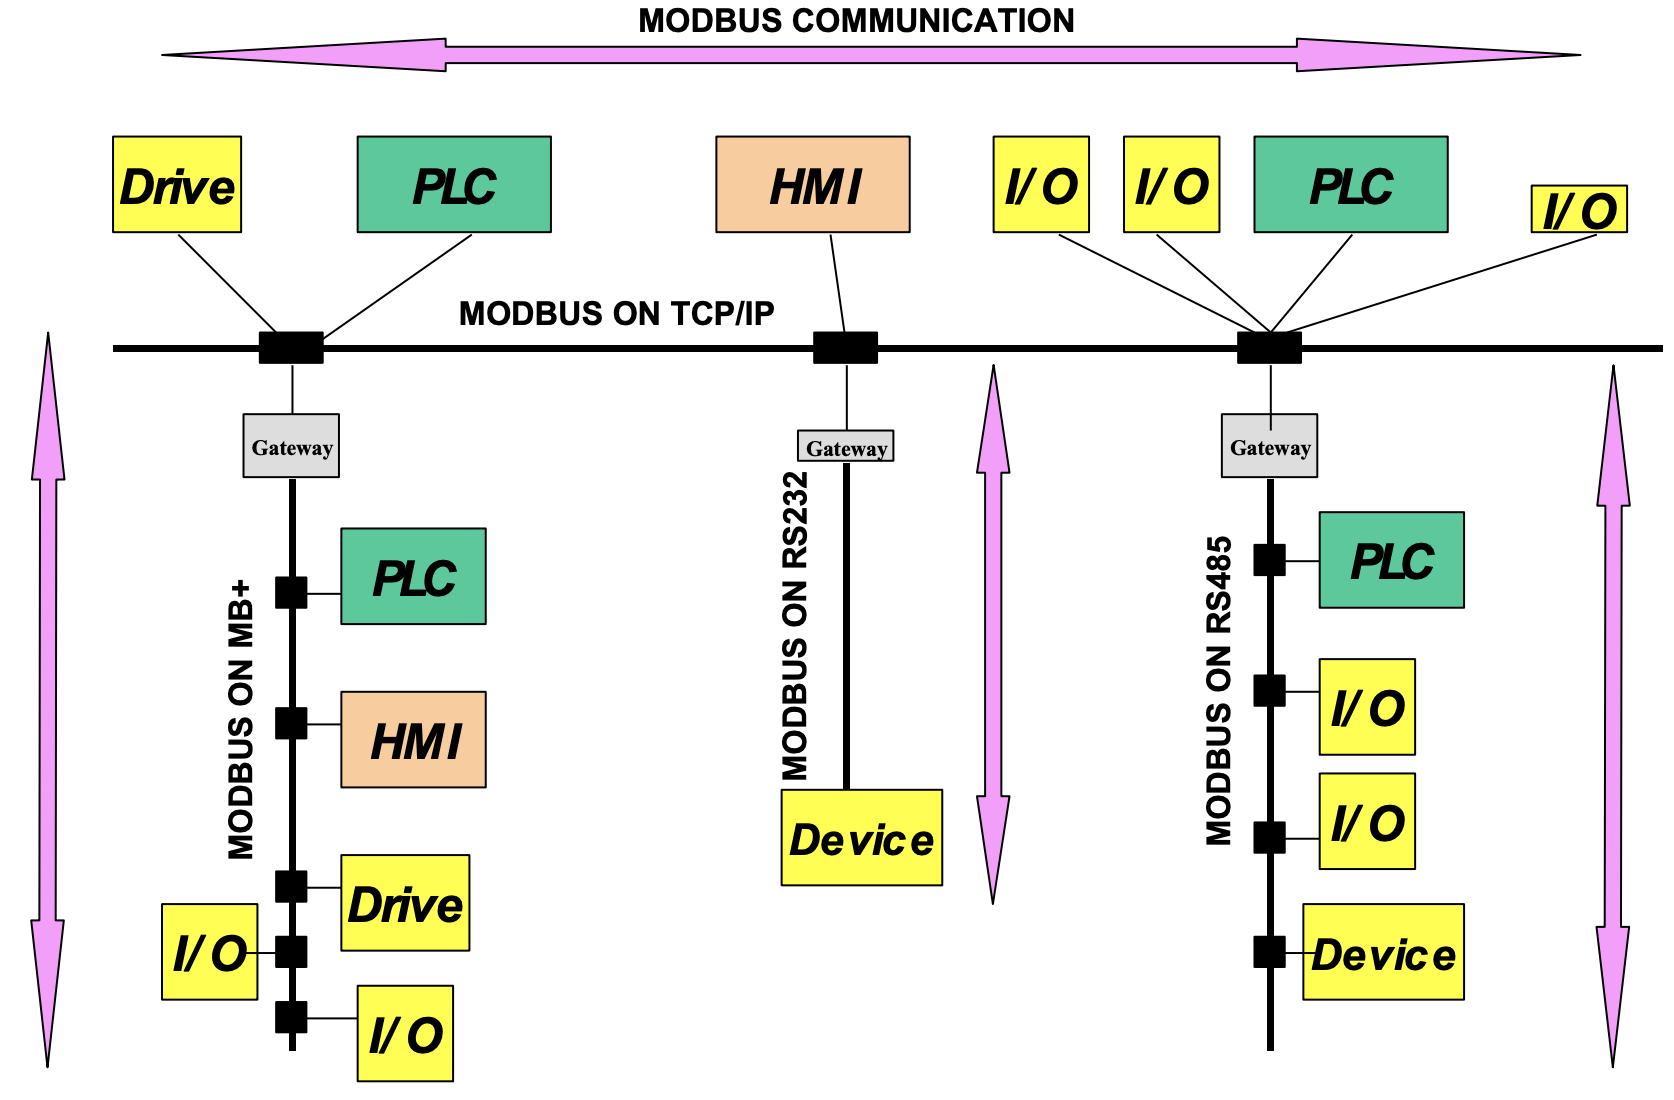
\includegraphics[scale=.35]{./Figures/red-modbus.png}
	\caption[Arquitectura de red Modbus.]{Ilustración de diferentes arquitecturas de red utilizando el protocolo Modbus\protect\footnotemark.}
	\label{fig:red-modbus}
\end{figure}

\footnotetext{\url{https://modbus.org/docs/Modbus_Application_Protocol_V1_1b3.pdf}}

Para la supervisión y control de un proceso industrial que utiliza Modbus como protocolo de comunicación,  se utilizan sistemas HMI (\textit{Human Machine Interface}) y hacen referencia a la manera que interactúa el humano con las diferentes máquinas que componen el sistema. 

Se trata de un sencillo panel que transmite órdenes, visualiza resultados de manera gráfica y obtiene visualización del estado del proceso o la máquina en tiempo real.  

A modo de ejemplo se pueden observar en la figura \ref{fig:hmi-siemens} diferentes modelos de HMI de la empresa Siemens. 

\begin{figure}[htpb]
	\centering
	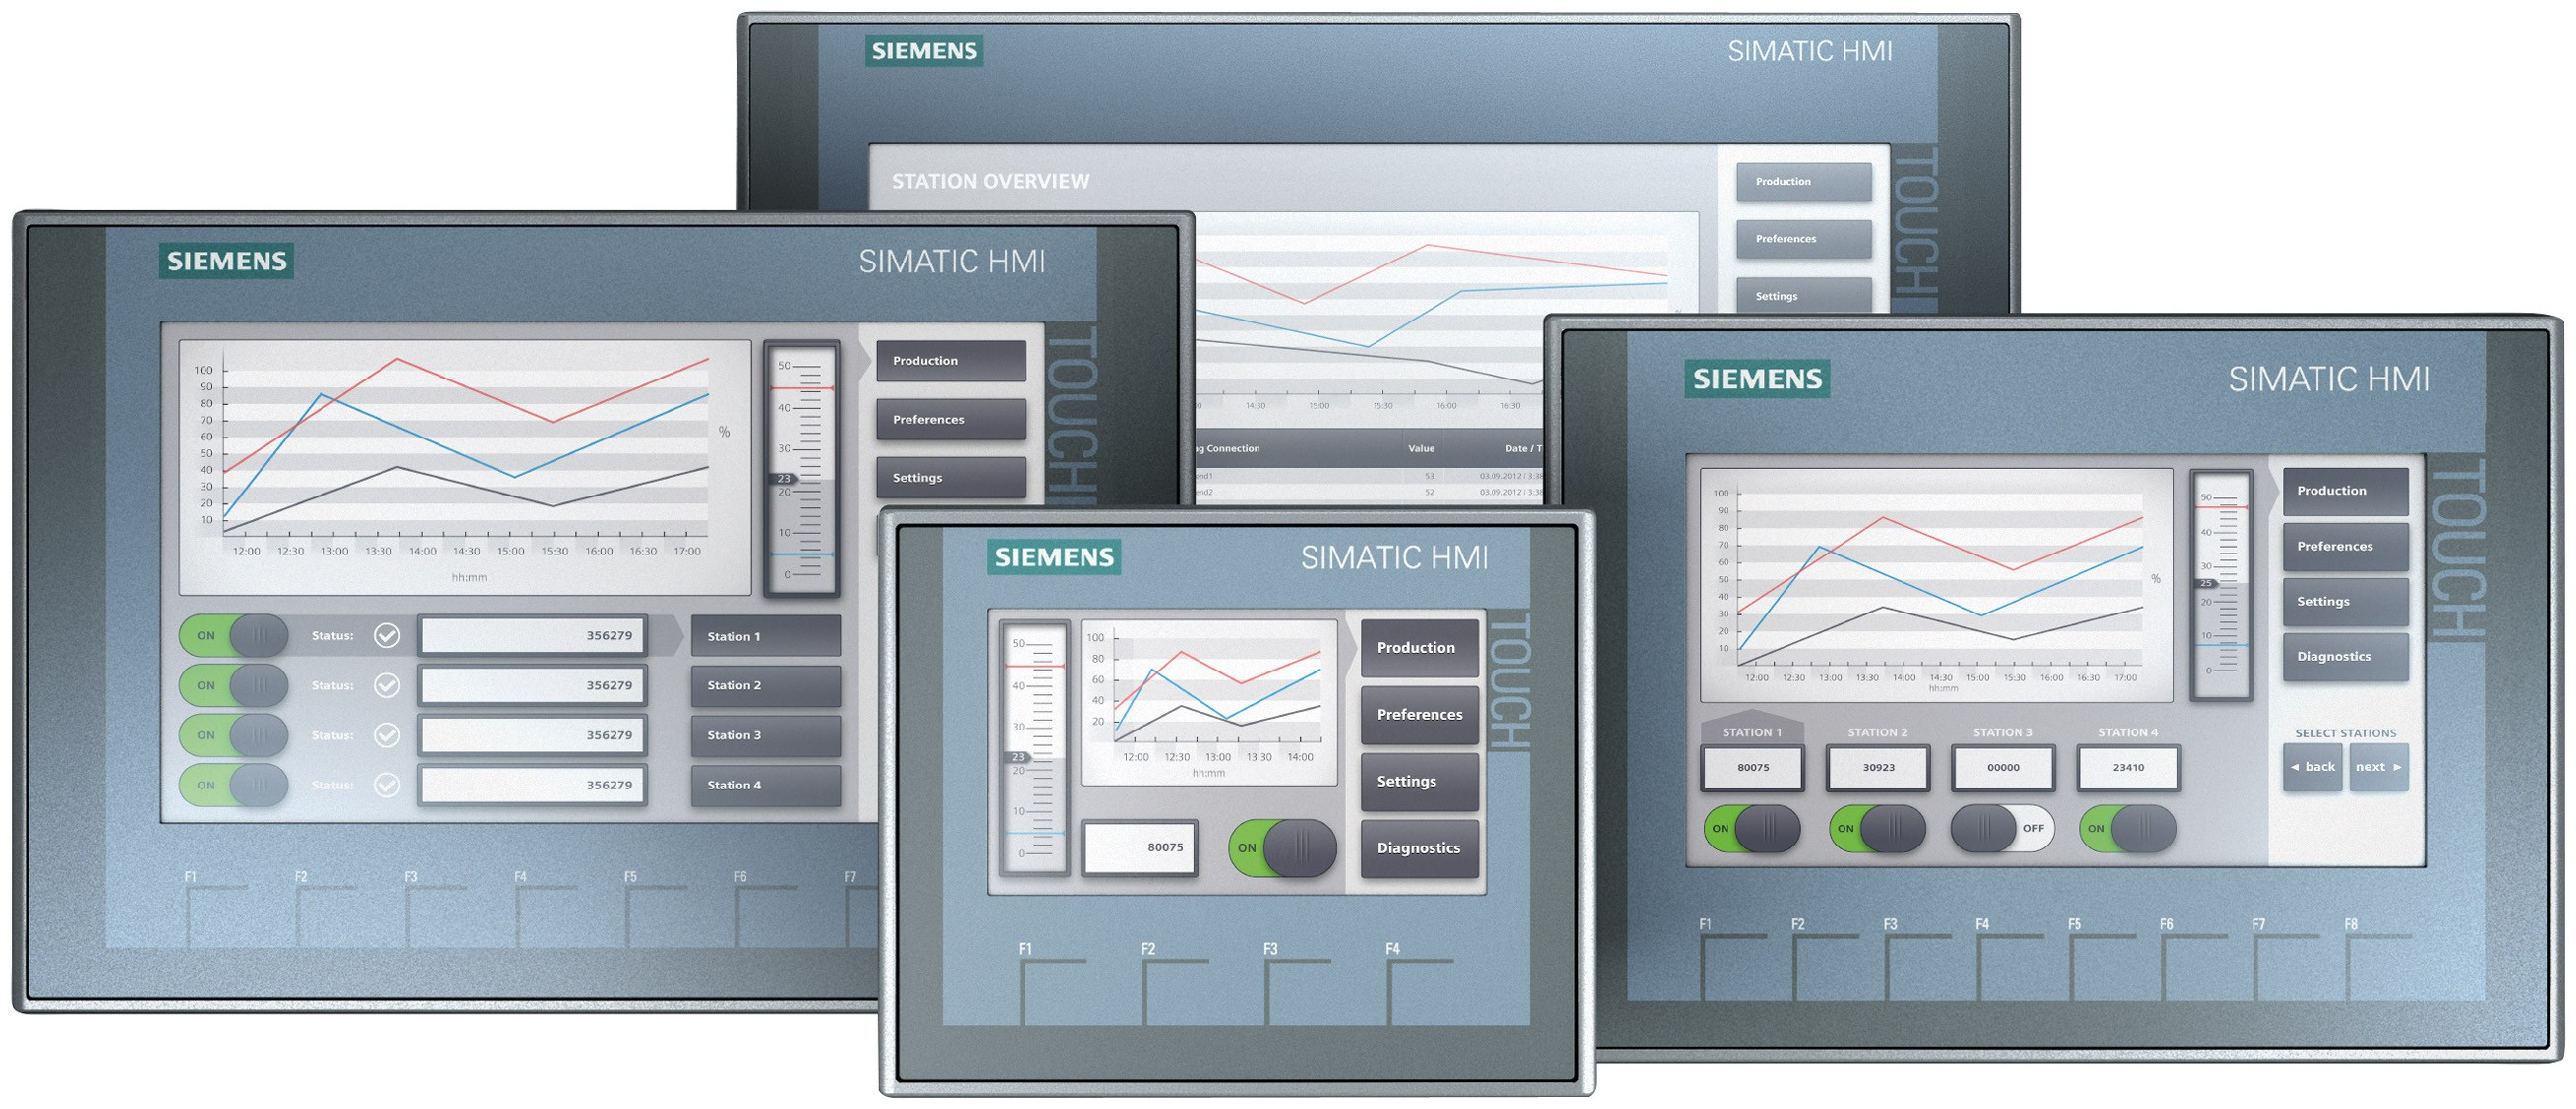
\includegraphics[scale=.10]{./Figures/hmi-ejemplos.jpg}
	\caption[Diferentes modelos de HMI de la empresa Siemens]{Diferentes modelos de HMI de la empresa Siemens\protect\footnotemark.}
	\label{fig:hmi-siemens}
\end{figure}

\footnotetext{\url{https://new.siemens.com/global/en/products/automation/simatic-hmi/panels/basic-panels.html}}

En un nivel superior de gestión del proceso industrial antes mencionado, se encuentra el sistema SCADA,  cuya palabra es un acrónimo que deriva del inglés  \textit{Supervisory Control And Data Acquisition} y su significado en español se traduce como Control Supervisor y Adquisición de Datos.

Los sistemas SCADA son programas de software que se utilizan para gestionar y controlar sistemas remotos o locales mediante el uso de una interfaz gráfica que comunica al usuario con el programa.  Cuentan con una estructura que parte de sus controladores lógicos programables (PLC) o unidades de terminal remotas (RTU)\citep{BOOK:1}, es decir, de microordenadores que se comunican con múltiples objetos, ya sean máquinas, dispositivos, sensores o HMI. Estos microordenadores después de comunicar, envían la información desde estos objetos a los ordenadores con el software SCADA.  

Por lo tanto, el sistema SCADA procesa, distribuye y muestra los datos, permitiendo a los operadores y otros trabajadores realizar un análisis para facilitar la toma de decisiones. Entre sus principales características, podemos destacar:

\begin{itemize}
	\item Supervisar remotamente las instalaciones y equipos.
	\item Monitorizar y controlar las operaciones en tiempo real.
	\item Procesar datos que hagan más fácil la toma de decisiones.
	\item Mostrar a través de imágenes dinámicas el comportamiento de los procesos.
	\item Arrojar señales de alarma (visuales o sonoras) frente a imprevistos.
\end{itemize}

En la figura \ref{fig:wincc-siemens} se puede observar la implementación de un sistema SCADA realizado con el software WINCC \citep{WEBSITE:4}  de la empresa Siemens para el monitoreo y gestión de energía eléctrica. 

\begin{figure}[htpb]
	\centering
	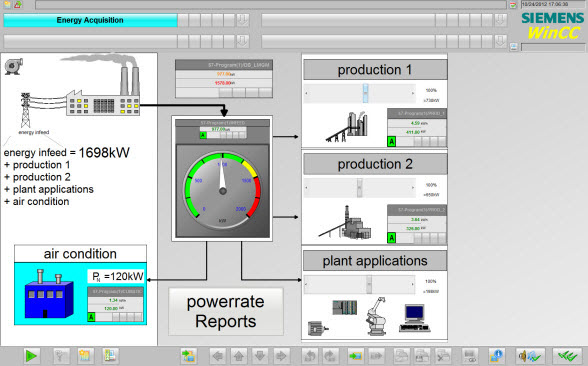
\includegraphics[scale=.7]{./Figures/wincc-siemens.jpg}
	\caption[Implementación de sistema SCADA con WINCC]{Ejemplo de implementación de un sistema SCADA con el software WINCC de la empresa Siemens para monitoreo y gestión de energía eléctrica\protect\footnotemark.}
	\label{fig:wincc-siemens}
\end{figure}

\footnotetext{\url{https://support.industry.siemens.com/cs/document/65384955/gestión-de-energía}}

%----------------------------------------------------------------------------------------

%\section{IIoT}

%----------------------------------------------------------------------------------------
\section{Internet de las cosas}

Por lo general, el término Internet de las cosas (IoT) se refiere a escenarios en los que la conectividad de red y la capacidad de cómputo se extienden a objetos, sensores y artículos de uso diario que habitualmente no se consideran computadoras, permitiendo que estos dispositivos generen, intercambien y consuman datos con una mínima intervención humana.  

El concepto de combinar computadoras, sensores y redes para monitorear y controlar diferentes dispositivos ha existido durante décadas. Sin embargo, la reciente confluencia de diferentes tendencias del mercado tecnológico está permitiendo que la internet de las cosas esté cada vez más cerca de ser una realidad generalizada.  

Estas tendencias incluyen la conectividad omnipresente, la adopción generalizada de redes basadas en el protocolo IP \citep{WEBSITE:9}, la economía en la capacidad de cómputo, la minimización, los avances en el análisis de datos y el surgimiento de la computación en la nube.

Los beneficios que internet de las cosas ofrece tanto a empresas como a personas individuales son numerosos. Desde un punto de vista económico, permite a las empresas gestionar y controlar mejor sus procesos de forma remota y en tiempo real, aumentando su eficiencia y posibilitando la toma de mejores decisiones y acciones preventivas como el mantenimiento de la maquinaria o sistemas instalados. En definitiva, esto conlleva un ahorro de costos y tiempo para la organización. En el caso de individuos particulares, los beneficios se traducen en mejoras de su calidad de vida y comodidad en el día a día mediante automatizaciones en su entorno cotidiano.

Las implementaciones de la IoT utilizan diferentes modelos de conectividad, cada uno de los cuales tiene sus propias características. Los cuatro modelos de conectividad descritos por la Junta de Arquitectura de Internet (IAB)\citep{WEBSITE:5} se mencionan en la siguiente lista:

\begin{itemize}
	\item \textit{Device-to-Device} (dispositivo a dispositivo).
	\item \textit{Device-to-Gateway} (dispositivo a puerta de enlace).
	\item \textit{Device-to-Cloud} (dispositivo a la nube).
	\item \textit{Back-End Data-Sharing} (intercambio de datos a través del backend).
\end{itemize}

Estos modelos destacan la flexibilidad en las formas en que los dispositivos de la IoT pueden conectarse y proporcionar un valor para el usuario.

La irrupción de la Internet de las cosas en la industria, tiene como objetivo conseguir una apertura total en la conectividad, es decir, la interconexión de todos los agentes que intervienen en la cadena del proceso productivo. Los dispositivos IoT serán capaces de capturar y analizar los datos obtenidos para tomar decisiones en tiempo real o enviarlos a la nube para almacenarlos y analizarlos mediante técnicas de \textit{big data}  e inteligencia artificial. Los empleos mas comunes en la industria pueden ser:
\begin{itemize}
	\item Obtención de valores de parámetros físicos y actuación sobre máquinas.
	\item Toma de datos para mantenimiento predictivo. 
	\item Control de la eficiencia energética mediante sensores.
	\item Automatización de procesos manuales y obtención de datos relevantes a través de sistemas embebidos.
	\item Comunicación Hombre – Máquina, notificaciones de alarmas, visualización de datos en tiempo real mediante \textit{wearables}.
\end{itemize}

La importancia de la internet de las cosas en el mundo de las empresas y las personas, queda reflejado en el crecimiento exponencial de dispositivos IoT conectados en el mundo, como se visualiza en la figura  \ref{fig:iot-crecimiento}. Para este año, se prevé que cerca de 36 mil millones de dispositivos IoT se encuentren en funcionamiento en el mundo, cifra que se extiende hasta los más de 75 mil millones para el año 2025.

\begin{figure}[htpb]
	\centering
	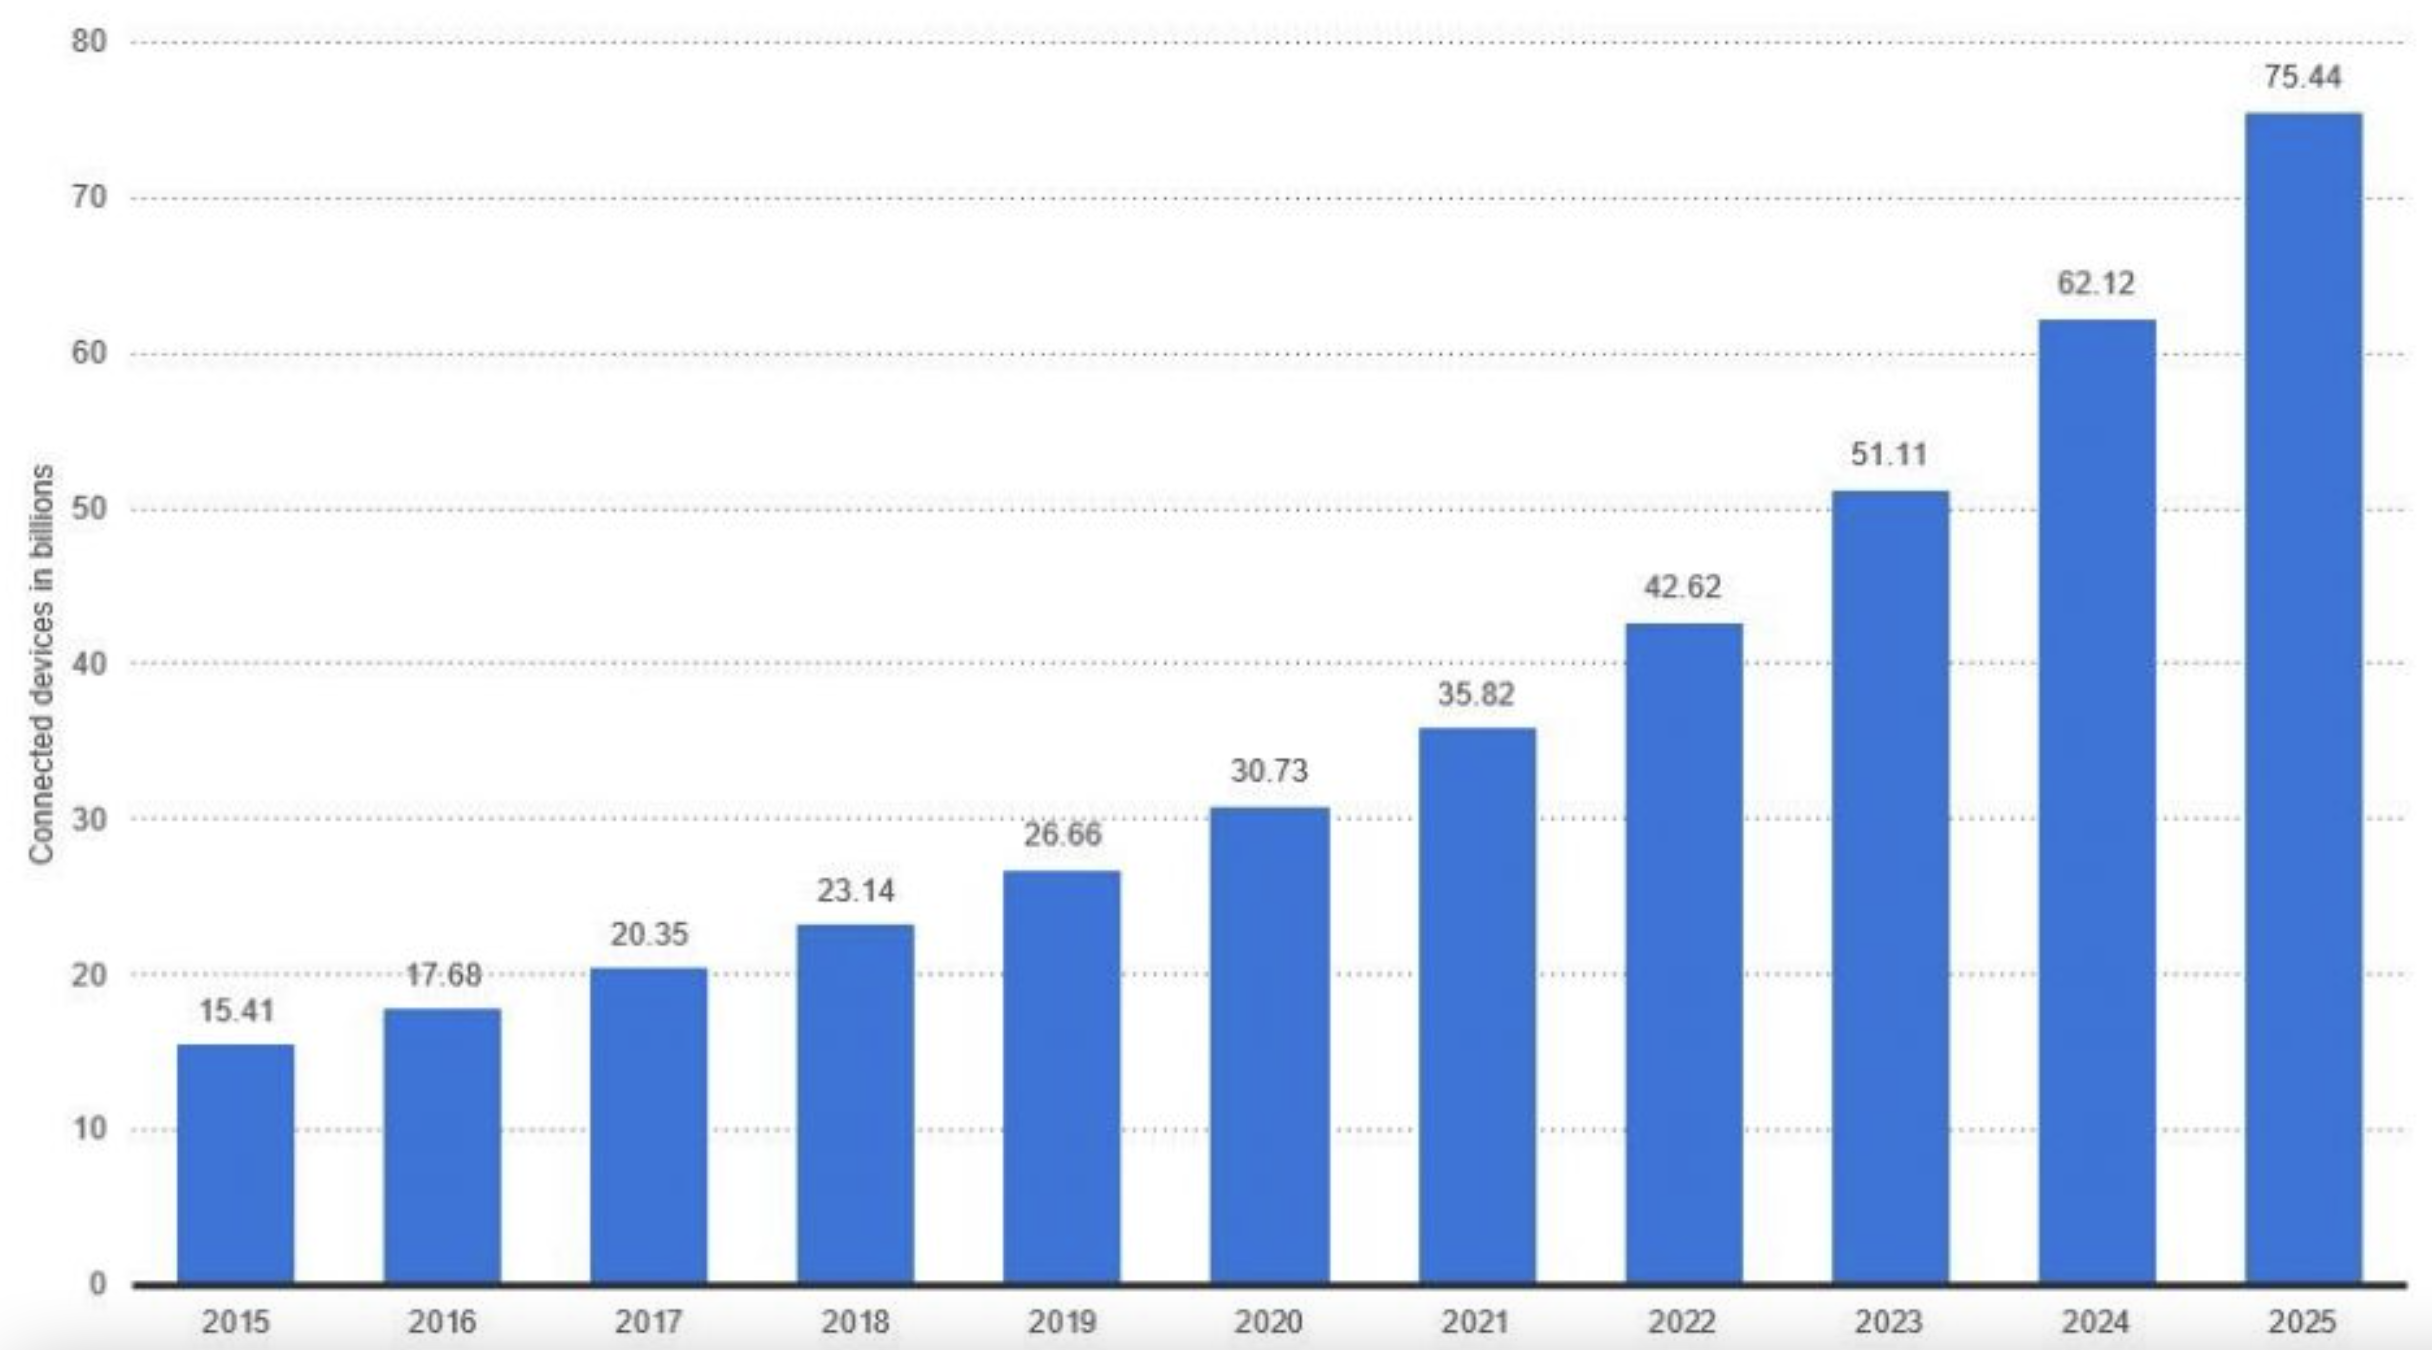
\includegraphics[scale=.3]{./Figures/iot-crecimiento.png}
	\caption[Crecimiento de dispositivos IoT]{Crecimiento exponencial de dispositivos conectados en el mundo\protect\footnotemark.}
	\label{fig:iot-crecimiento}
\end{figure}

\footnotetext{\url{https://www.iotworldonline.es/las-grandes-estadísticas-del-internet-de-las-cosas-iot/}}

%----------------------------------------------------------------------------------------

%\section{IEstado del arte}

%----------------------------------------------------------------------------------------
\section{Estado del arte}
\label{sec:estado-arte}
En la actualidad existen varias plataformas cloud que brindan un conjunto de servicios de computación en la nube para hacer frente a las necesidades del negocio en lo que respecta al desarrollo de aplicaciones, almacenamiento y cómputo. 

Algunas de las que se encuentran consolidadas a nivel mundial son: Google, Microsoft, Amazon, Samsung, entre otras \citep{WEBSITE:6}.  Estos sistemas, si bien tienen toda la infraestructura realizada para conectar dispositivos IoT, requieren de desarrollo web que implica la programación de toda la estructura de la información que se requiere enviar a la nube.  Por otro lado,  no todas las empresas implementan como protocolo de aplicación a MQTT \citep{WEBSITE:7}.  Se resumen algunos servicios ofrecidos por estas empresas en la tabla \ref{tab:cloud-emp}.

\begin{table}[h]
	\centering
	\caption[Comparación de servicios cloud en el mercado.]{Comparación de servicios cloud en el mercado.}
	\begin{tabular}{l c c c}    
		\toprule
		\textbf{Empresa} 	 & \textbf{Servicios} 		& \textbf{Protocolo}     & \textbf{Sistema}\\
		 	 						 & \textbf{Cloud} 		& \textbf{de aplicación}     & \textbf{operativo}\\
		\midrule
		Google 			& Google Cloud 				& Weave 		& Linux\\		
		Amazon	 	& AWS IoT						& MQTT		& Linux\\
		Microsoft	 	& Azure IoT						& AMQP 		& Windows IoT\\
		Samsung	 	& SmartThings					& MQTT 		& Linux\\
		\bottomrule
		\hline
	\end{tabular}
	\label{tab:cloud-emp}
\end{table}

En cuanto a plataformas que ofrecen la etapa de procesamiento, análisis y visualización de datos, se pueden mencionar algunas como ThingBoard, Ubidots, NodeRed, entre otras. Estas plataformas asumen que el cliente cuenta con el hardware necesario para enviarles la información relevante, y ellas se encargan de analizarla y presentarla de manera conveniente mediante tableros o dashboards, que le permiten al usuario ver el estado e históricos de sensores, actuadores y nodos. 

Las principales desventajas de estas plataformas son la fuerte dependencia que generan y la poca adaptabilidad al hardware que se requiere gestionar, además la mayoría de ellas brindan servicios con costos monetarios elevados.

%----------------------------------------------------------------------------------------

%\section{Motivacion}

%----------------------------------------------------------------------------------------
\section{Motivación}

En la actualidad existen múltiples dispositivos conversores de protocolos que permiten enviar datos a la nube, pero la mayoría no posee un sistema de gestión a través de una plataforma web. La metodología de conexión es a través de la vinculación con servicios web como los mencionados en la sección \ref{sec:estado-arte} donde el usuario deberá encargarse de realizar todo el desarrollo de la visualización de datos en forma clara, el almacenamiento de datos en una base de datos y la generación de eventos que puedan serle útil. 

Empresas multinacionales como ser ABB, Scheider Electric, Honeywell o Siemens,  poseen sus propias plataformas web de gestión y protocolos de comunicación, lo que genera un sistema cerrado y dependiente de un determinado fabricante de dispositivos, por lo que imposibilita la conexión de conversores de otras marcas. 

Por estos motivos antes mencionados, surgió la posibilidad de ofrecer un servicio de gestión web, que contenga todos los componentes necesarios para que el usuario solo requiera de una configuración básica de conexión al servidor y en un breve periodo de tiempo, pueda visualizar los datos requeridos de forma remota, pudiendo generar reportes y almacenamiento de datos. 

%----------------------------------------------------------------------------------------

%\section{Alcances y objetivos}

%----------------------------------------------------------------------------------------
\section{Alcances y objetivos}

\subsection{Objetivos}

El propósito de este proyecto,  es el desarrollo de un sistema que contenga un servidor MQTT, una base de datos para alojar información de reportes de dispositivos y una plataforma web que permita visualizar de forma remota datos enviados de diferentes sensores que contengan instalado un conversor de protocolo Modbus a MQTT.  Esto permitirá maximizar la eficiencia del proceso, ya que puede ser monitoreado en tiempo real desde cualquier parte del mundo, contando con avisos de alarmas, reportes históricos y almacenamiento de datos. 

\subsection{Alcance}

Para la realización de este trabajo se propuso desarrollar una plataforma web operativa de un sistema de gestión para conversores de protocolo Modbus a MQTT que se conectan a sensores de temperatura fabricados por la empresa D\&T \citep{WEBSITE:8}.  El presente desarrollo incluye los siguientes aspectos:

\begin{itemize}
	\item Implementación de servidor MQTT.
	\item Implementación de servidor para gestión de usuarios y dispositivos.
	\item Implementación de base de datos no relacional. 
	\item Visualización de datos en tiempo real en una plataforma web. 
	\item Lectura de datos provenientes de sensores de temperatura que contenga un conversor de protocolo Modbus a MQTT.
\end{itemize}

\chapter{Introducción específica} % Main chapter title

\label{Chapter2}

En este capítulo se exponen las características del software utilizado para la programación del sistema, partiendo del backend hasta el frontend. También se identifican los módulos de funcionamiento del dispositivo conversor Modbus a MQTT utilizado en el trabajo.  Finalmente se describe la utilidad de Nginx como servidor de datos para integrar el sistema. 



%----------------------------------------------------------------------------------------
%	SECTION {Dispositivo conversor Modbus a MQTT}
%----------------------------------------------------------------------------------------
\section{Dispositivo conversor Modbus a MQTT}

El conversor consta de un circuito electrónico que actúa de interfaz de conexión entre aparatos o dispositivos que se encuentran en una red Modbus y posibilita la conversión de datos al protocolo MQTT a través de una conexión.

En la figura \ref{fig:dev-conv} se puede observar el diagrama de bloques con las partes más importantes que componen al dispositivo. 

\begin{figure}[htpb]
	\centering
	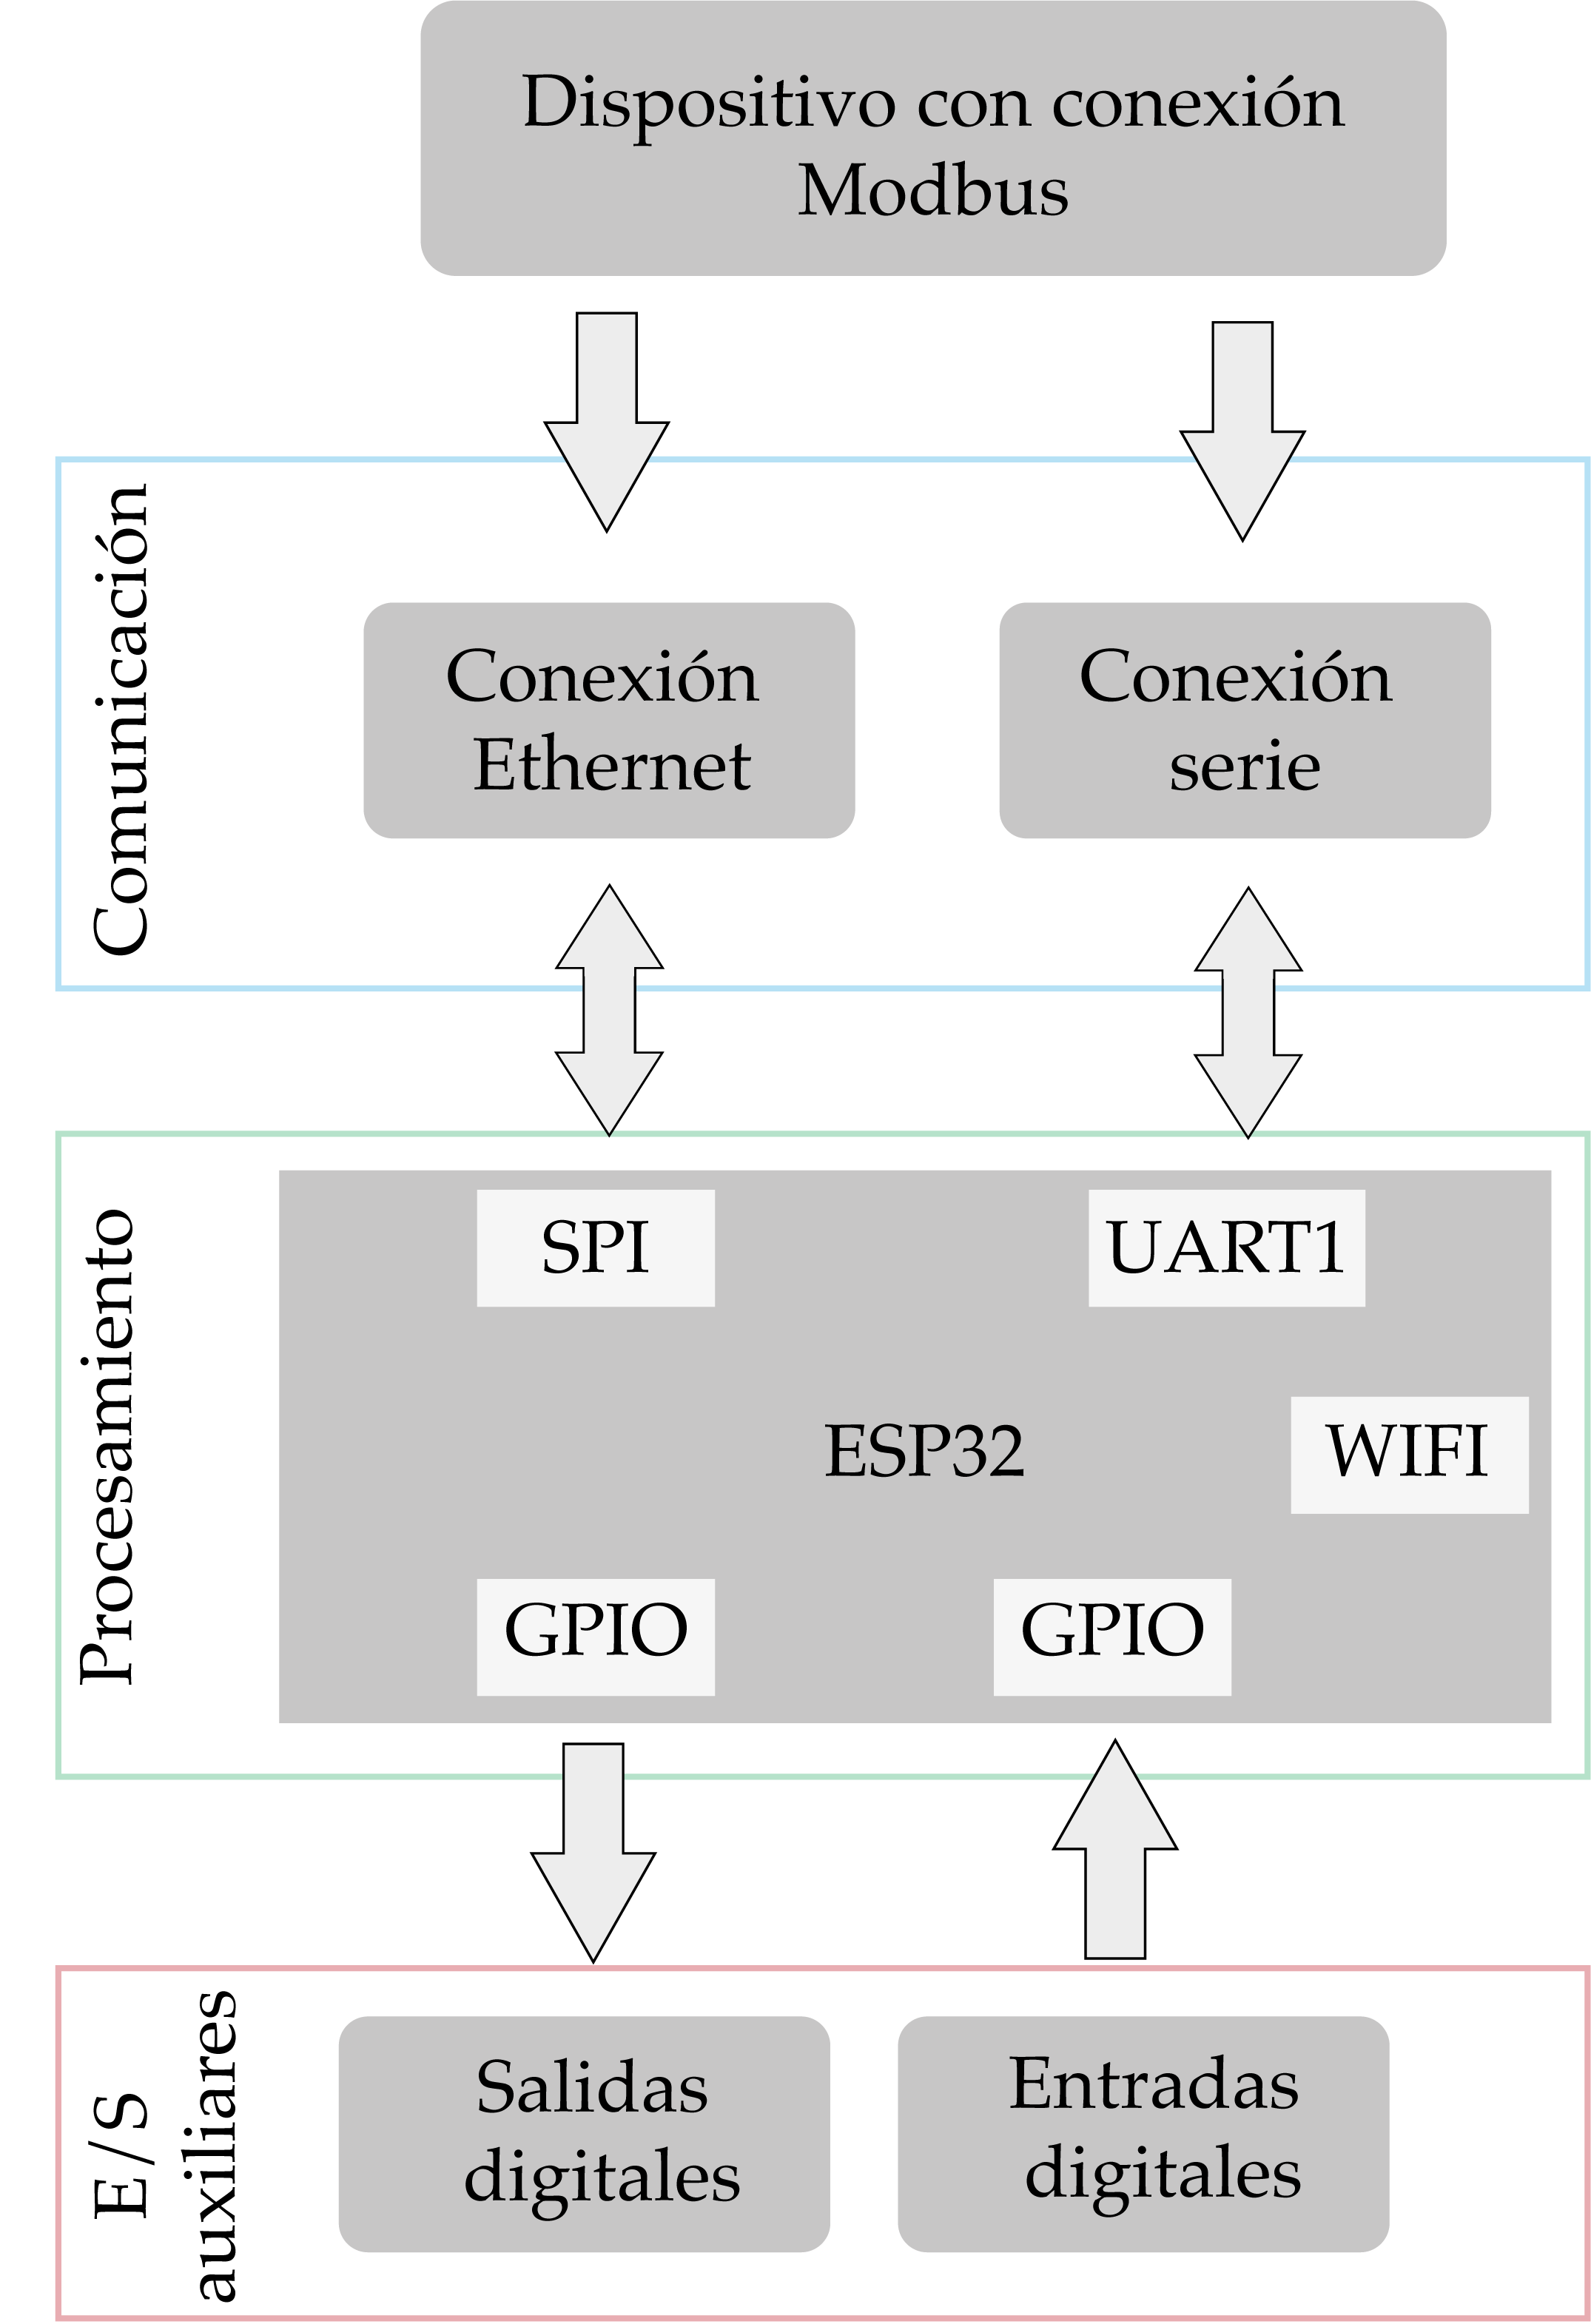
\includegraphics[scale=.35]{./Figures/diagrama_dispositivo.png}
	\caption[Diagrama de bloques de dispositivo conversor ]{Diagrama de bloques de dispositivo conversor Modbus a MQTT.}
	\label{fig:dev-conv}
\end{figure}

Al sistema se lo puede separar en tres grupos:

\begin{itemize}
	\item Comunicación: este bloque está compuesto por un circuito de conexión ethernet para poder recibir mensajes de dispositivos que están conectados a través de Modbus TCP. 
	
	Por otro lado el hardware contiene un circuito de conexión para dispositivos que se conectan por Modbus serie.
	
	\item Procesamiento: es el bloque principal donde se gestionan todos los datos recibidos por parte del módulo de comunicación y  convierte los mensajes Modbus para luego poder ser enviados por MQTT a través de Wi-Fi  
	
	Este módulo está constituido por un microcontrolador ESP32 \citep{WEBSITE:11} de la empresa Espressif \citep{WEBSITE:10} quien se encarga de controlar el módulo de comunicación y el módulo de entradas y salidas auxiliares.
	
	Los datos provenientes del módulo de comunicación son reconvertidos a un formato de datos del tipo JSON \citep{WEBSITE:12} para ser enviados vía Wi-Fi por protocolo MQTT.
	
	
	\item Entradas y salidas auxiliares: este bloque permite conectar dispositivos externos al conversor. 
	
	Como ejemplo se pueden mencionar sensores para las entradas y actuadores para las salidas. 
	
	
\end{itemize}


%----------------------------------------------------------------------------------------
%	SECTION {Protocolos}
%----------------------------------------------------------------------------------------
\section{Protocolos de comunicación}
En el caso de la comunicación con un servidor remoto se requiere tener acceso a Internet y por lo tanto es necesario conectarse también con un módem que a
su vez debe estar conectado a un proveedor de servicios de Internet (ISP, por sus siglas en inglés correspondientes a \textit{Internet Service Provider}).

Necesariamente para poder conectarse a Internet, el conversor de protocolo Modbus a MQTT debe implementar el protocolo TCP/IP \citep{WEBSITE:15} o UDP/IP \citep{WEBSITE:16}, que determinan las características de las capas de transporte y red del estándar OSI \citep{WEBSITE:13}. La capa de aplicación, ubicada en la parte superior del modelo, es la encargada de ofrecer a las aplicaciones de usuario la posibilidad de comunicarse con otros dispositivos a través de los servicios brindados por las demás capas. Entre los protocolos de aplicación, existen múltiples como AMQP, CoAP, DDS, STOMP, MQTT y HTTP, siendo estos dos últimos los utilizados en el trabajo realizado.

Ambos protocolos son ampliamente utilizados para aplicaciones en la internet de las cosas.  MQTT se basa en un modelo de publicaciones y suscripciones en el que un cliente publica mensajes en un tema o tópico y todos aquellos nodos que se encuentran suscritos a ese tema reciben el mensaje publicado. MQTT es ideal para aplicaciones de IoT debido principalmente a que requiere un muy bajo ancho de banda, tiene un menor consumo de potencia que otras alternativas y además es sencillo y ligero de implementar. 

Por otro lado, HTTP \citep{WEBSITE:14} (\textit{ Hypertext Transfer Protocol} ) nos permite realizar una petición de datos y recursos, como pueden ser documentos HTML \citep{BOOK:2}, y es la base de cualquier intercambio de datos en la web. La estructura está basada en cliente y servidor, esto quiere decir que una petición de datos es iniciada por el elemento que recibirá los datos (el cliente), normalmente un navegador web.   Así,  una página web completa resulta de la unión de distintos sub documentos recibidos, como ser un documento que especifique el estilo de maquetación de la página web, el texto, las imágenes, vídeos, scripts, entre otros. 

Clientes y servidores se comunican intercambiando mensajes individuales. Los mensajes que envía el cliente se llaman peticiones y los mensajes enviados por el servidor se llaman respuestas.


%----------------------------------------------------------------------------------------
%	SECTION {MQTT}
%----------------------------------------------------------------------------------------
\subsection{Protocolo MQTT}
\label{mqtt-section}
MQTT o \textit{ Message Queue Telemetry Transport} es un protocolo de transporte liviano de mensajes basado en un modelo de publicaciones y suscripciones como se ilustra en la figura \ref{fig:mqtt-esquema}. El protocolo MQTT funciona sobre TCP/IP o sobre otros protocolos de red con soporte bidireccional y sin pérdidas de datos.

\begin{figure}[htpb]
	\centering
	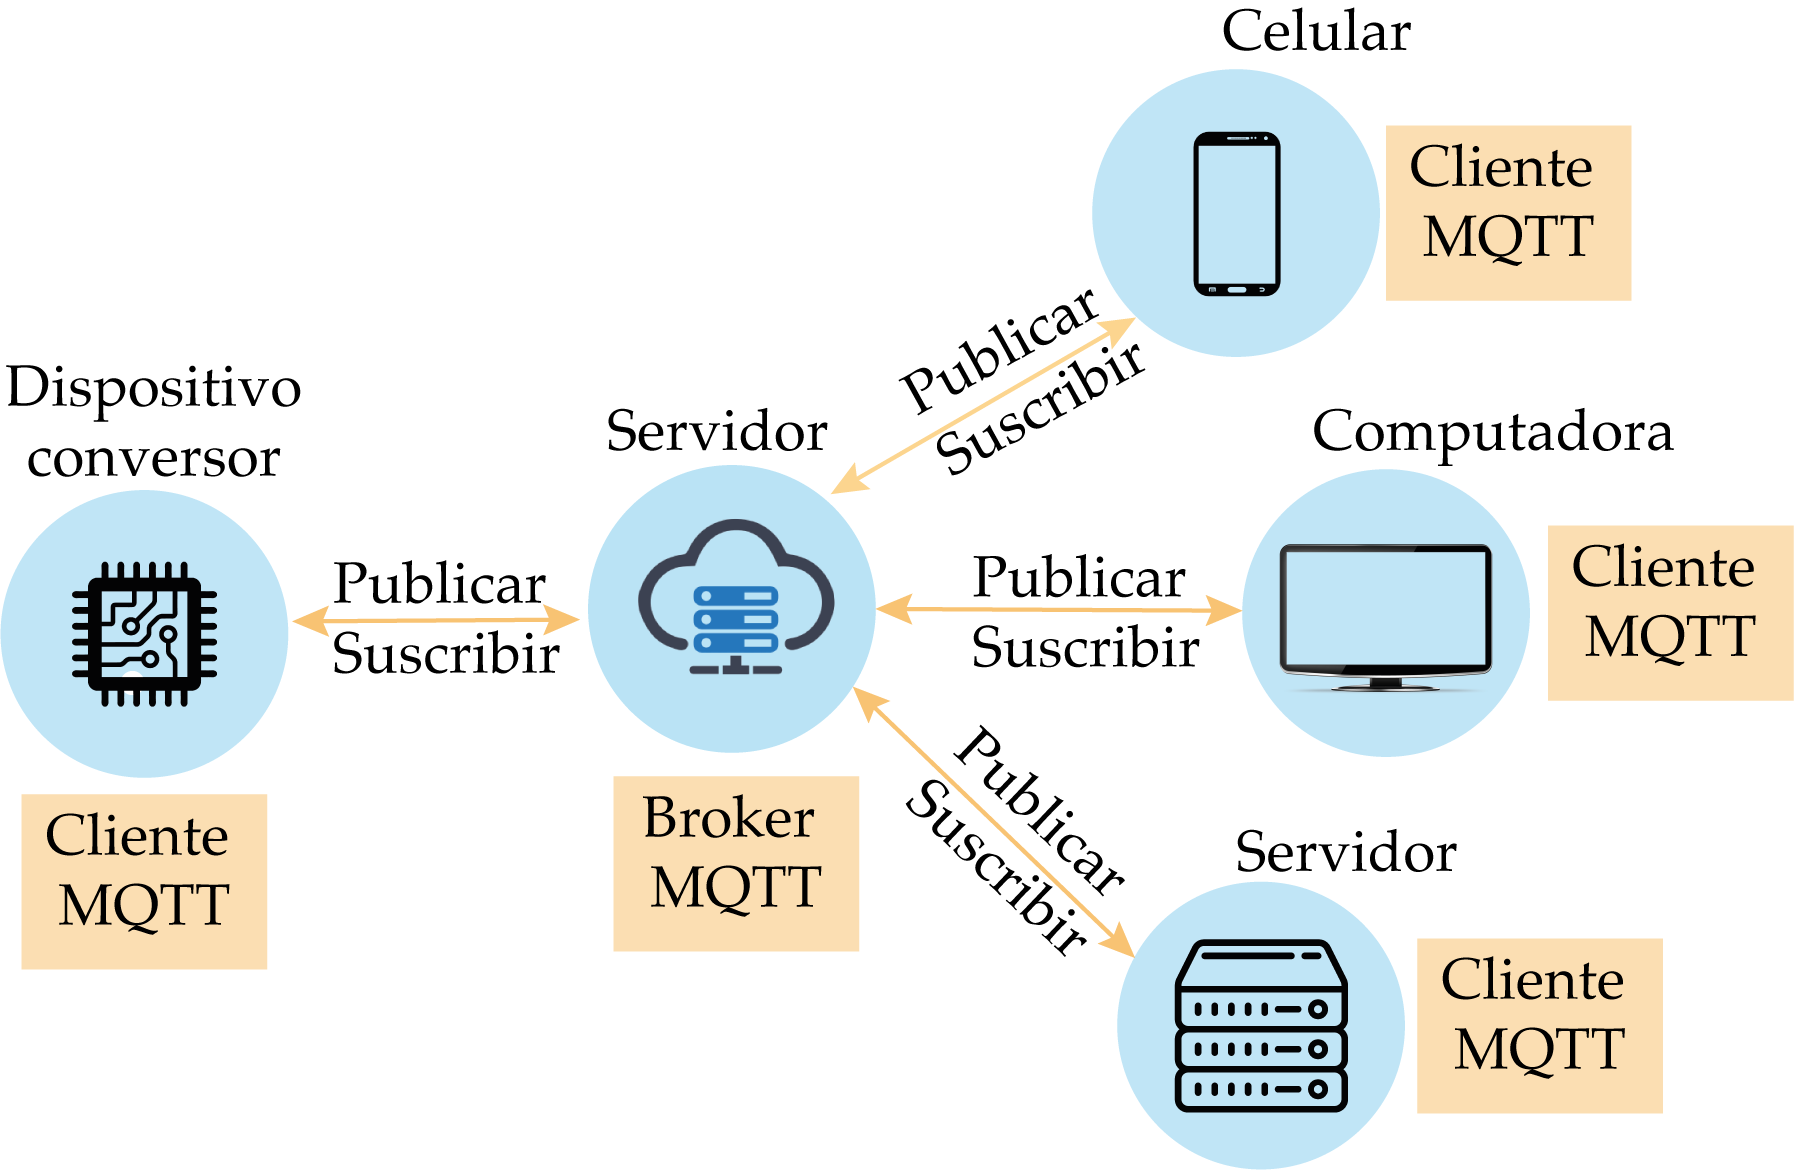
\includegraphics[scale=.7]{./Figures/mqtt-protocol.png}
	\caption[Esquema de funcionamiento MQTT ]{Modelo de funcionamiento de protocolo MQTT.}
	\label{fig:mqtt-esquema}
\end{figure}

En modelos del tipo publicación y suscripción, un dispositivo puede publicar un mensaje en un tema o tópico y/o suscribirse a un tópico particular para la recepción de mensajes.  A diferencia de un modelo cliente/servidor típico donde ambas partes se comunican directamente, en este esquema se desacopla tanto el cliente que envía un mensaje, como el o los clientes que están suscritos a dicho tópico y reciben ese mensaje. 

La conexión entre ambas partes es manejada por una tercera parte llamada broker MQTT.  El broker MQTT es el responsable de recibir todos los mensajes, filtrarlos y distribuirlos según corresponda, es decir, determinar qué cliente está suscrito a cada tópico y enviar los mensajes publicados en ellos a estos suscriptores.

La conexión en MQTT es siempre entre un cliente y el broker, como se ilustra en la figura \ref{fig:mqtt-cliente-broker} es decir que los clientes nunca se conectan entre ellos directamente.

\begin{figure}[htpb]
	\centering
	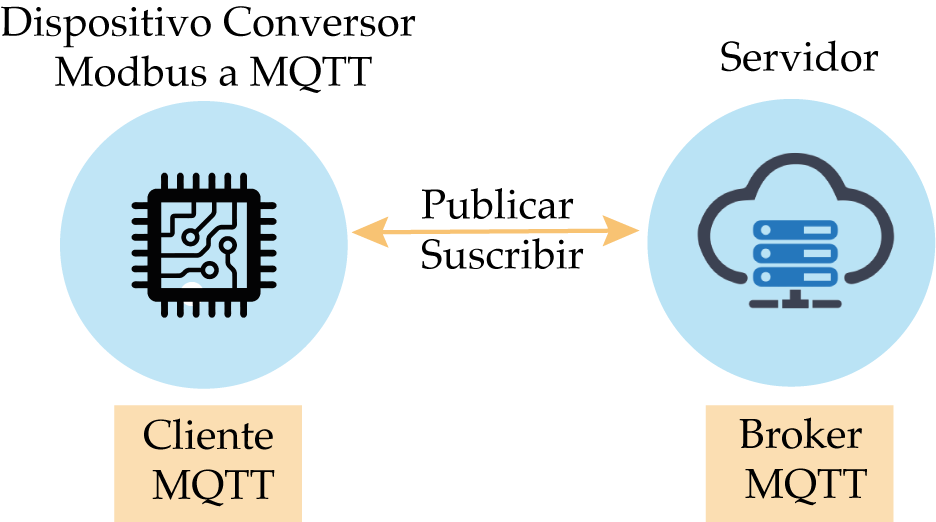
\includegraphics[scale=.7]{./Figures/cliente-broker.png}
	\caption{Esquema de conexión cliente - broker MQTT.}
	\label{fig:mqtt-cliente-broker}
\end{figure}

Para iniciar una conexión, el cliente envía un mensaje CONNECT al broker y este responde con un mensaje CONNACK y un código de estado. Una vez que la conexión queda establecida, el broker la mantiene abierta hasta que el cliente envía un comando de desconexión o la conexión se pierde por algún motivo. Los puertos estándar son 1883 para comunicación no encriptada y 8883 para comunicación encriptada usando SSL/TLS \citep{WEBSITE:17}.

Durante el handshake SSL/TLS, el cliente valida el certificado del servidor para autenticarlo. El cliente puede también proveer un certificado al broker durante el handshake, que el broker utilizará para autenticar al cliente. Si bien no es parte de la especificación, se ha vuelto habitual que los brokers admitan la autenticación de clientes con certificados SSL/TLS. Debido a que el protocolo MQTT apunta a ser un protocolo para dispositivos de IoT con recursos limitados, SSL/TLS puede no ser siempre una opción, y en algunos casos, puede que no sea deseable. En tales casos, la autenticación se presenta como un nombre de usuario y una contraseña de texto simple que el cliente envía al servidor como parte de la secuencia de paquetes CONNECT/CONNACK.  En el caso del presente trabajo, se optó utilizar autenticación mediante nombre de usuario y contraseña y certificado SSL para el cliente web.

Los mensajes son la información que se quiere intercambiar entre los dispositivos, ya sean comandos o datos. En MQTT la palabra tópico refiere a una cadena de caracteres que el broker utiliza para filtrar mensajes para cada cliente conectado. Los tópicos consisten en uno o más niveles. Cada nivel de tópico está separado por una barra. Existen algunos caracteres reservados que son utilizados como comodines o \textit{wildcards} que permiten la suscripción a múltiples tópicos, como el carácter '+' y el carácter '\#', que representan el  \textit{wildcards} de nivel único y de nivel múltiple, respectivamente. En cualquier caso, no es necesario que los clientes creen previamente el tópico antes de publicar o suscribirse a él. El broker acepta cada tópico válido sin previa inicialización.

Ejemplos de tópicos y uso de los wildcards son provistos en la figura \ref{fig:mqtt-wildcards}:

\begin{figure}[htpb]
	\centering
	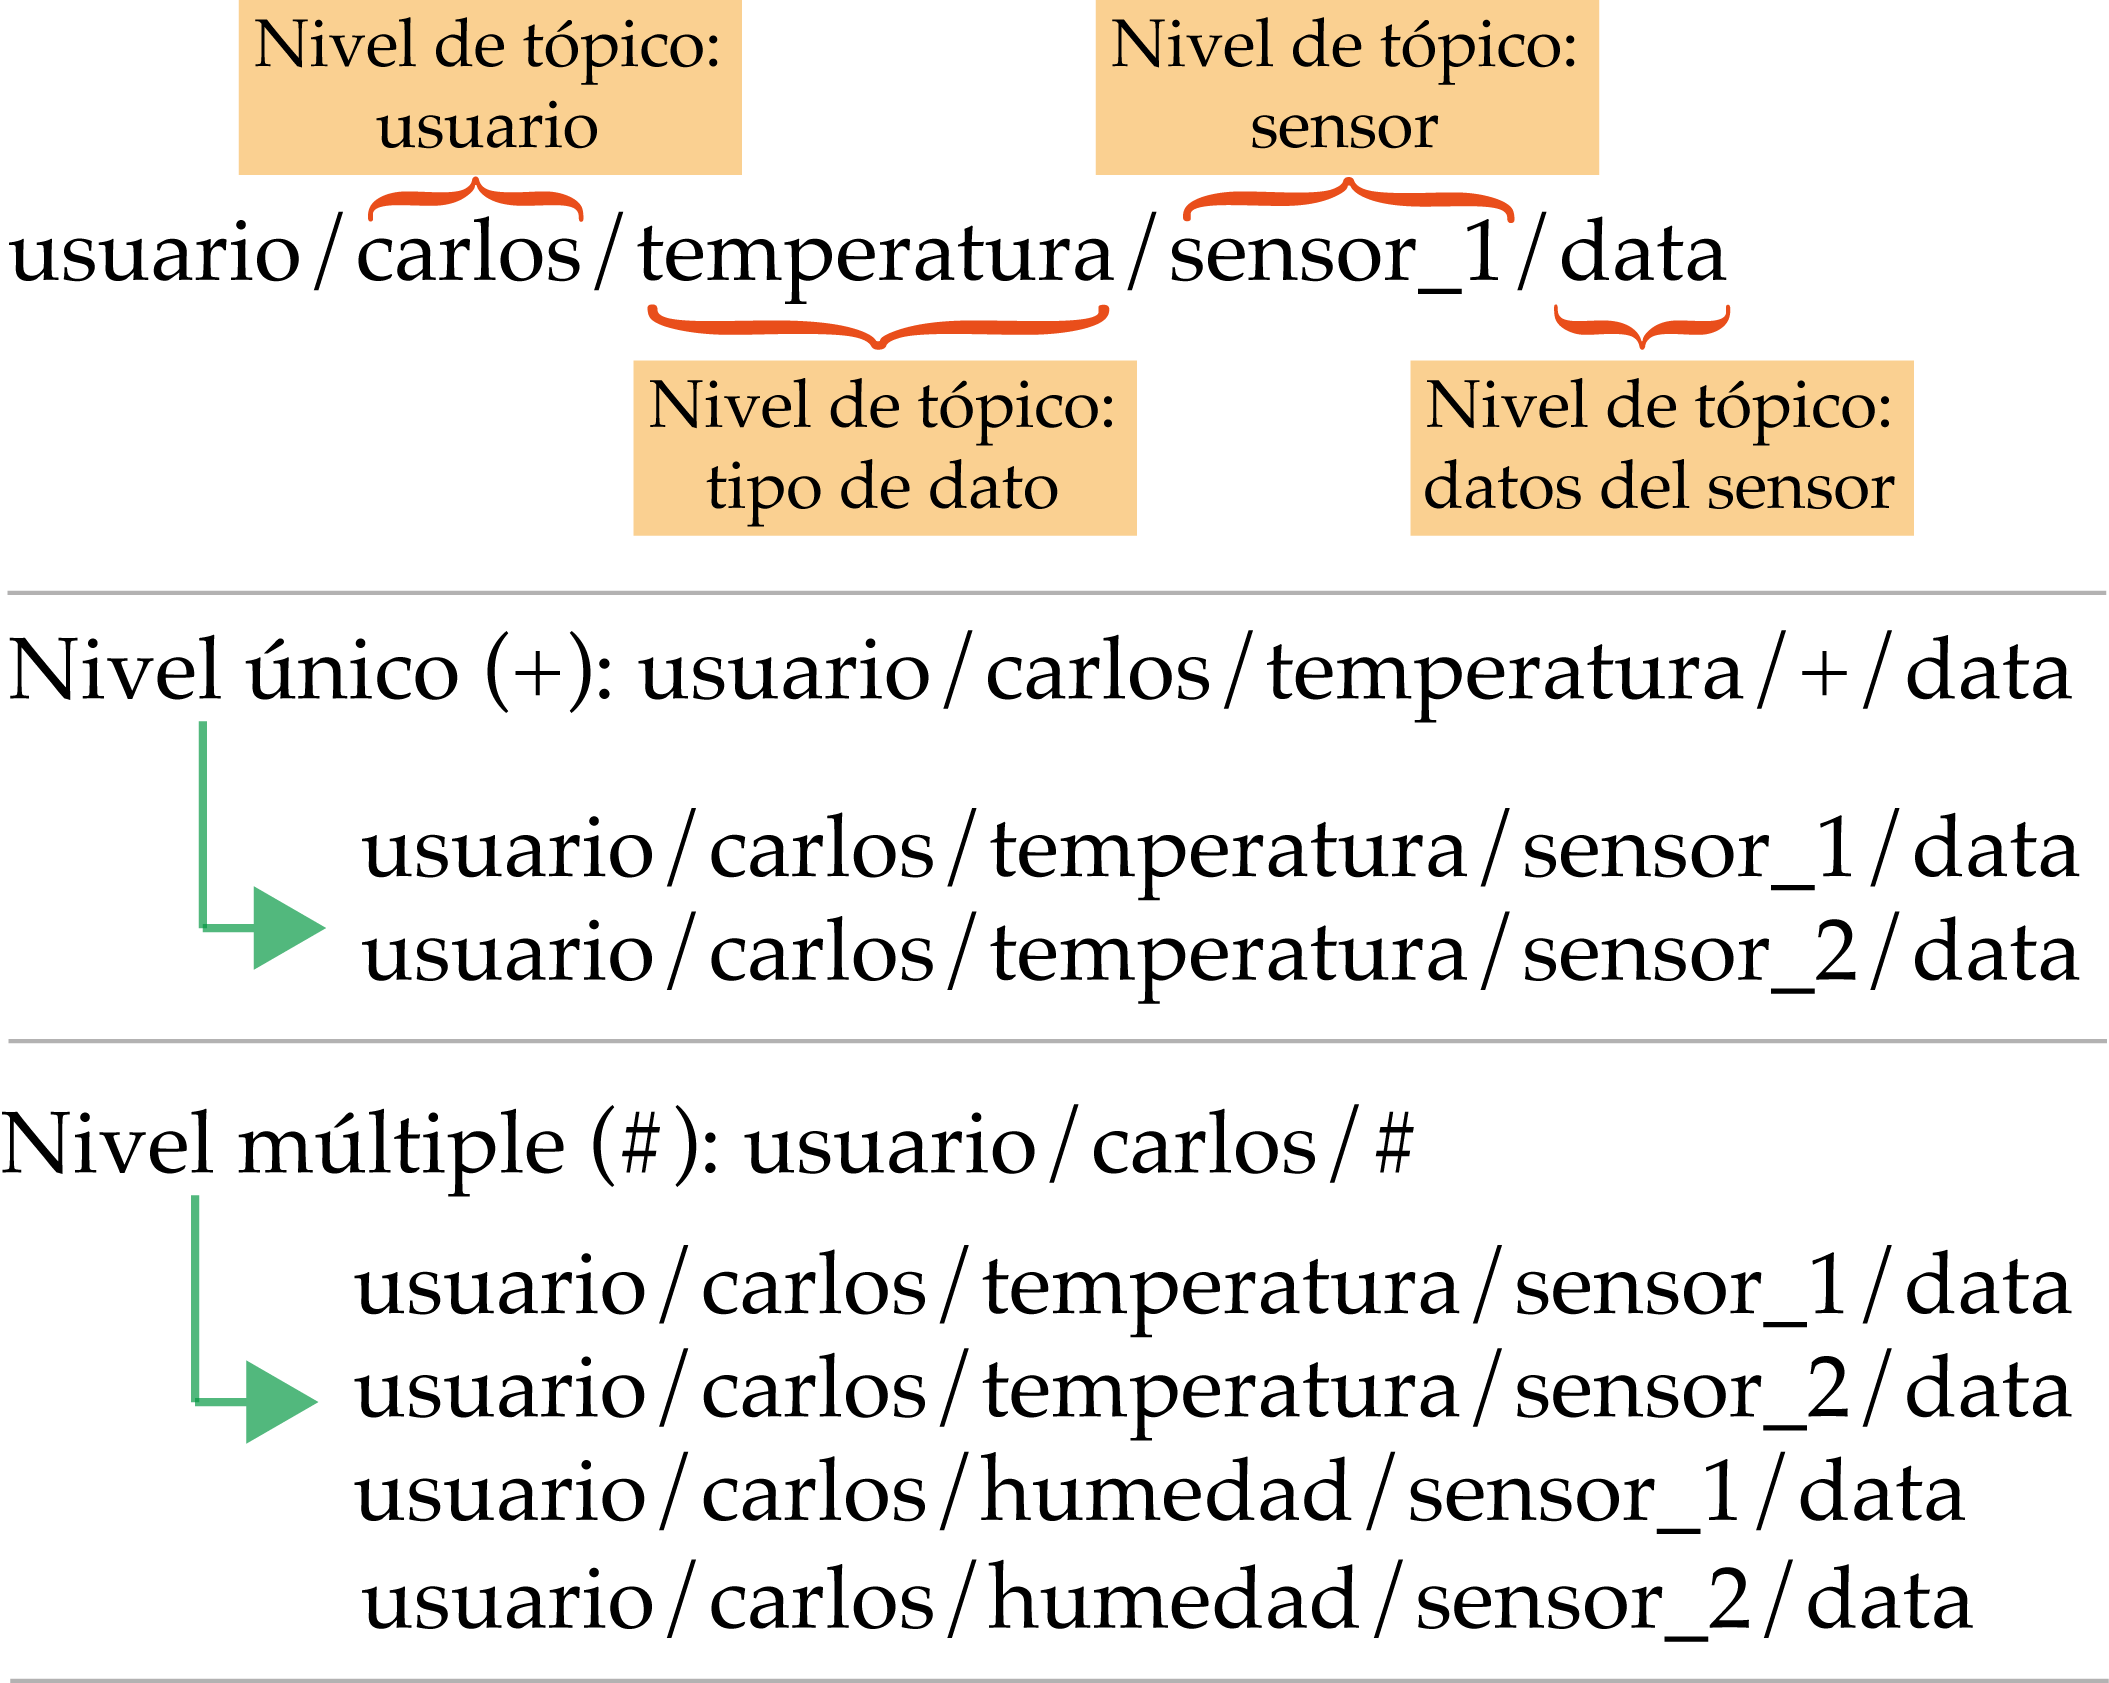
\includegraphics[scale=.38]{./Figures/esquema-wildcard.png}
	\caption{Ejemplo de tópicos y uso de \textit{wildcards}.}
	\label{fig:mqtt-wildcards}
\end{figure}



%----------------------------------------------------------------------------------------
%	SECTION {Protocolo HTTP}
%----------------------------------------------------------------------------------------
\subsection{Protocolo HTTP}

Diseñado a principios de la década de 1990, HTTP es un protocolo ampliable que ha ido evolucionando con el tiempo. Es lo que se conoce como un protocolo de la capa de aplicación, y se transmite sobre el protocolo TCP, o el protocolo encriptado TLS, aunque teóricamente podría usarse cualquier otro protocolo fiable. 

Gracias a que es un protocolo capaz de ampliarse, se usa no solo para transmitir documentos de hipertexto (HTML), si no que además se usa para transmitir imágenes o vídeos, o enviar datos o contenido a los servidores, como en el caso de los formularios de datos. HTTP puede incluso ser utilizado para transmitir partes de documentos, y actualizar páginas web en el acto.

Es un protocolo basado en el principio de cliente-servidor donde las peticiones son enviadas por una entidad llamada agente de usuario (del ingles \textit{user agent}). La mayoría de las veces el agente de usuario o cliente,  es un navegador web. Cada petición individual se envía a un servidor, el cuál la gestiona y responde. Entre cada petición y respuesta, hay varios intermediarios, normalmente denominados proxies \citep{WEBSITE:18} , los cuales realizan distintas funciones, como \textit{gateways} o caches.  En la figura  \ref{fig:server-proxy} se puede visualizar un caso típico de aplicación de utilización de proxy como \textit{gateway}.

\begin{figure}[htpb]
	\centering
	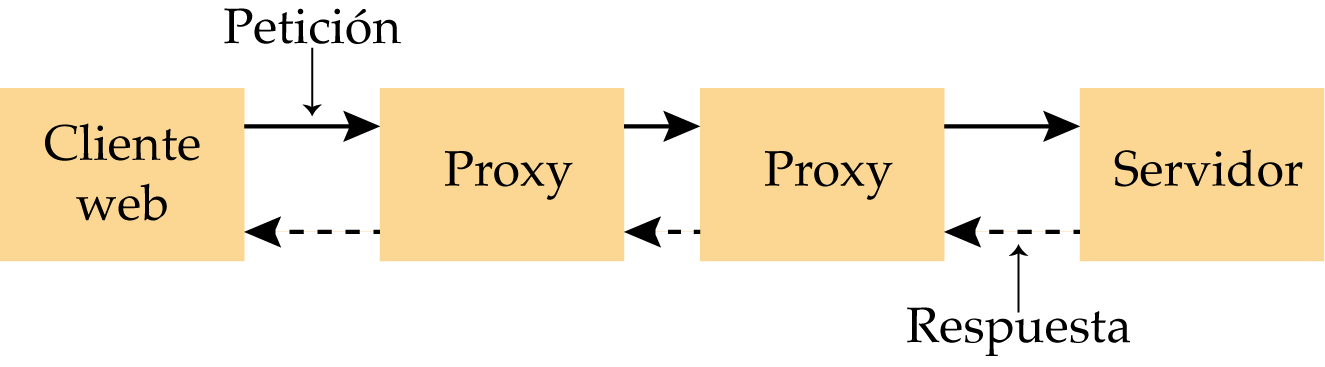
\includegraphics[scale=.80]{./Figures/server-proxy.png}
	\caption[Utilización de proxy como  \textit{gateway}.  ]{Diagrama de bloques ilustrando la utilización de proxy como  \textit{gateway}.}
	\label{fig:server-proxy}
\end{figure}


El navegador es siempre el que inicia una comunicación (petición), por lo que para poder mostrar una página web, envía una petición de documento HTML al servidor. Entonces procesa este documento y envía más peticiones para solicitar scripts, hojas de estilo y otros datos que necesite. El navegador, une todos estos documentos y datos y como resultado se obtiene la pagina web. 

Al otro lado del canal de comunicación está el servidor, el cual sirve los datos que ha pedido el cliente. Un servidor conceptualmente es una única entidad, aunque puede estar formado por varios elementos que se reparten la carga de peticiones (\textit{load balancing}), u otros programas que gestionan otras computadoras como cache, bases de datos, servidores de correo electrónico, entre otros y que generan parte o todo el documento que ha sido pedido. 

Una petición de HTTP está formada por los siguientes campos:

\begin{itemize}
	\item Un método HTTP: normalmente pueden ser un verbo, como: GET, POST o un nombre como OPTIONS o HEAD que defina la operación que el cliente quiera realizar. El objetivo de un cliente, suele ser una petición de recursos, usando GET, o presentar un valor de un formulario HTML, usando POST, aunque en otras ocasiones puede hacer otros tipos de peticiones. 
	
	\item La dirección del recurso pedido: la URL del recurso.
	
	\item La versión del protocolo HTTP.
	
	\item Cabeceras HTTP opcionales que pueden aportar información adicional a los servidores.
	
	\item O un cuerpo de mensaje, en algún método como puede ser POST, en el cual envía la información para el servidor.
	
\end{itemize}

A modo de ejemplo, en la figura \ref{fig:peticiones-http}  se puede observar una petición GET al servidor utilizado en este trabajo.

\begin{figure}[htpb]
	\centering
	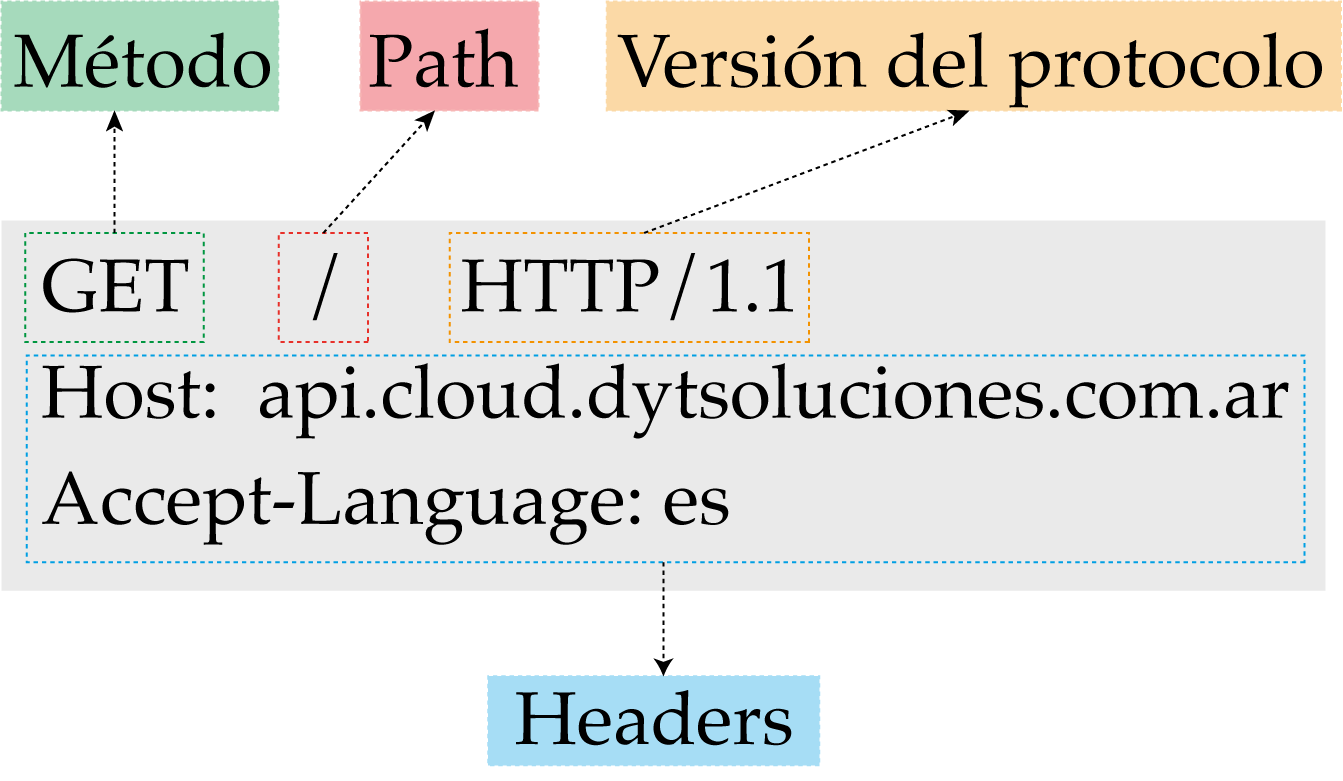
\includegraphics[scale=.50]{./Figures/peticion-http.png}
	\caption[Petición GET al servidor ]{Ejemplo de petición GET al servidor utilizado para realizar este trabajo.}
	\label{fig:peticiones-http}
\end{figure}


Por otro lado, las respuestas están formadas por los siguientes campos:

\begin{itemize}
	\item La versión del protocolo HTTP que se usa.
	
	\item Un código de estado, indicando si la petición ha sido exitosa.
	
	\item Un mensaje de estado, una breve descripción del código de estado.
	
	\item Cabeceras HTTP, como las de las peticiones.
	
	\item Opcionalmente, el recurso que se ha pedido.
	
\end{itemize}

En la figura \ref{fig:respuesta-http}  se observa un modelo de respuesta para ejemplificar los campos más importantes: 

\begin{figure}[htpb]
	\centering
	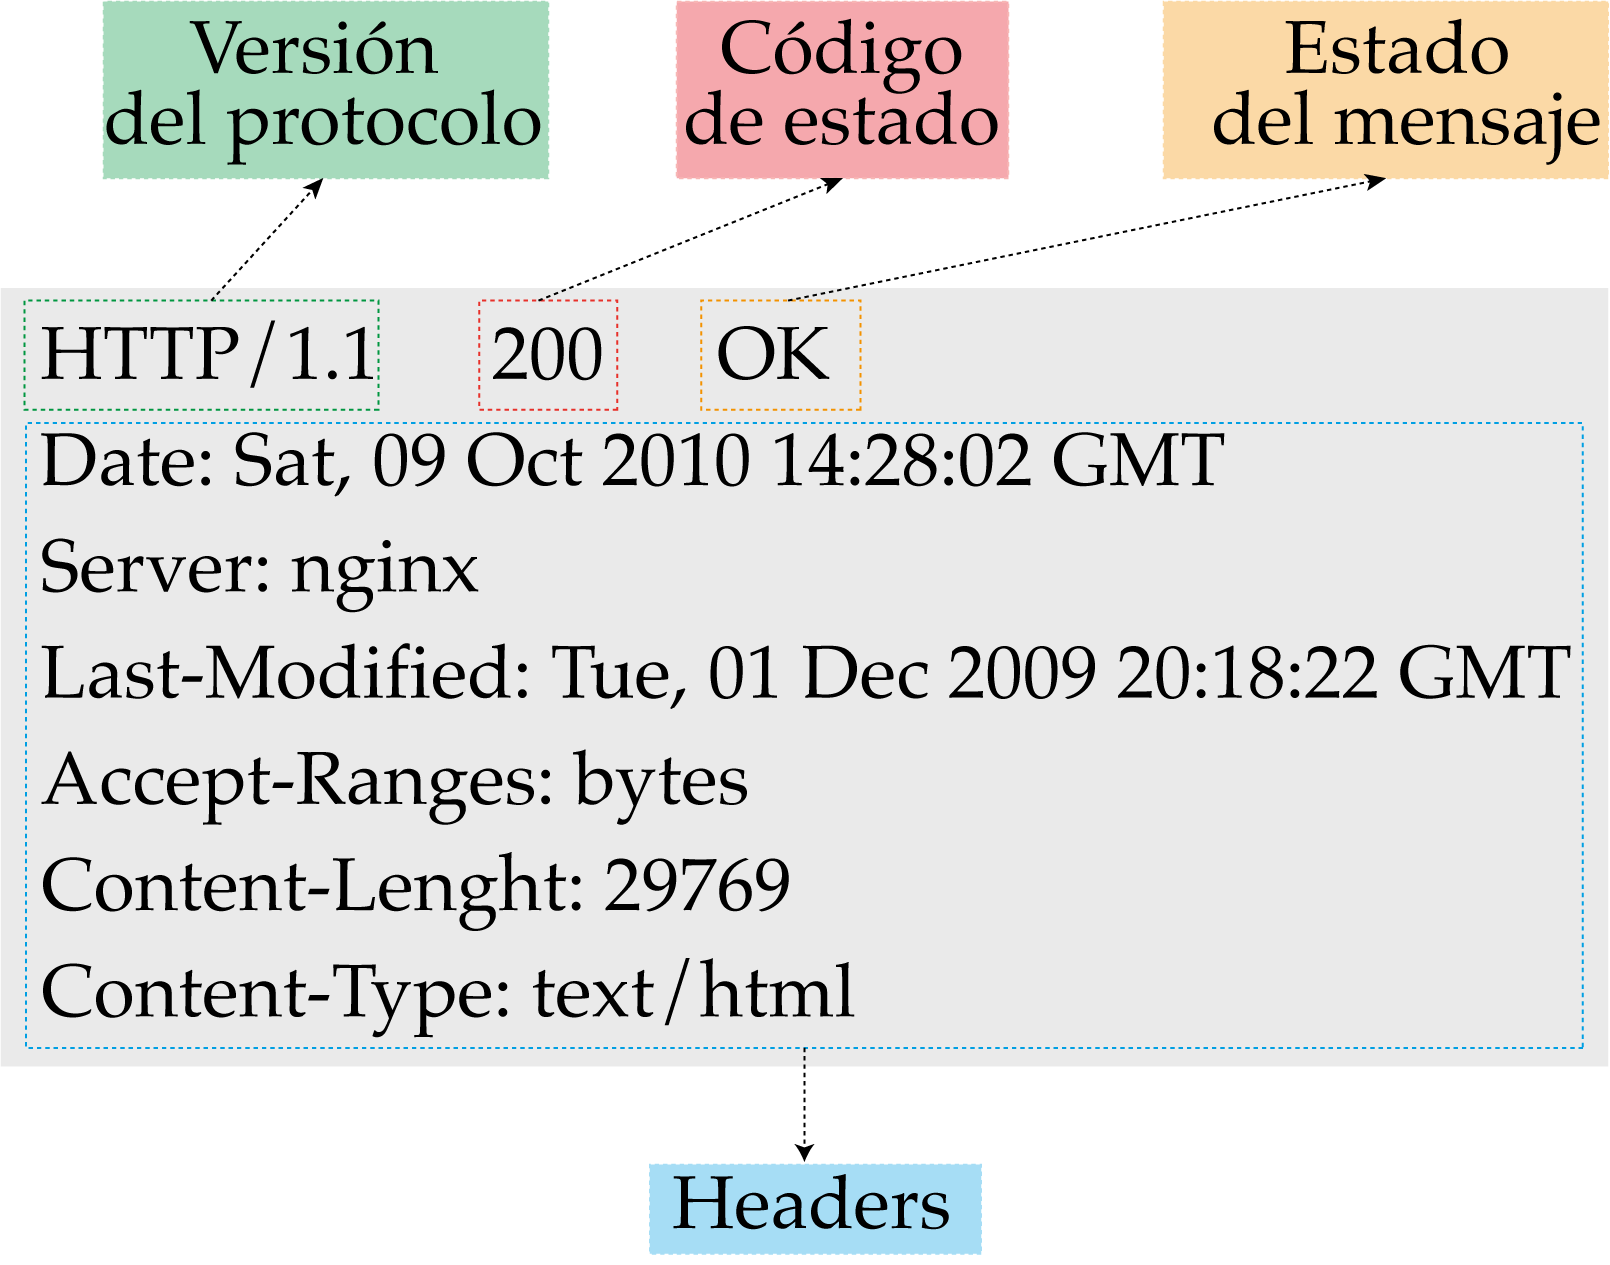
\includegraphics[scale=.50]{./Figures/respuesta-http.png}
	\caption[Modelo de respuesta HTTP ]{Ejemplo de modelo de respuesta HTTP del servidor.}
	\label{fig:respuesta-http}
\end{figure}


%----------------------------------------------------------------------------------------
%	SECTION {Backend}
%----------------------------------------------------------------------------------------
\section{Infraestructura del backend}

En informática, la expresión backend hace referencia a la parte de la infraestructura de datos de un sistema que se encuentran generalmente en el servidor y se encarga de procesar y almacenar información.  Las funciones más importantes del backend son las siguientes:

\begin{itemize}
	\item Acceder a la información que se pide a través de la plataforma web: cuando se usa una aplicación web, se solicita información de manera continua. Esto implica que el sistema tiene que ser capaz de encontrar y acceder a lo solicitado a través de funciones de consulta. 
	
	\item Combinar la información encontrada y transformarla: una vez encontrada, el backend combina la información para que resulte útil al usuario.
	
	\item Devolver la información al usuario:  finalmente, el backend envía la información relevada de vuelta al usuario. 
	
\end{itemize}

En este trabajo el backend consiste en un servidor, una aplicación web y una base de datos y debe cumplir con los siguientes criterios:

\begin{itemize}
	\item Escalabilidad: hace referencia a la flexibilidad del mismo para integrar nuevas estructuras y códigos si el futuro la aplicación lo requiere.
	
	\item Seguridad: debido a la constante interacción del backend con la base de datos, se debe hacer uso de conexiones seguras como HTTPS.
	
	\item Robustez: es la capacidad para funcionar en cualquier contexto ante situaciones inesperadas.
	
\end{itemize}

Para el desarrollo del backend del trabajo se utilizó el \textit{framework} Node.js \citep{WEBSITE:19} ,  el cual fue ideado como un entorno de ejecución de JavaScript orientado a eventos asíncronos. Está diseñado para crear aplicaciones de red escalables.

Además de la alta velocidad de ejecución, Node.js dispone del bucle de eventos (\textit{Event Loop}), que permitirá gestionar enormes cantidades de clientes de forma asíncrona. Tradicionalmente para trabajar de forma asíncrona las aplicaciones se valían de la programación basada en hilos (\textit{programming threaded applications}), pero esto supone la utilización de un espacio de memoria que va escalando a medida que la cantidad de clientes conectados a la aplicación aumenta, por lo tanto si se necesita gestionar grandes cantidades de conexiones habrá que ampliar el número de servidores.

Para el almacenamiento de los datos se utilizó MongoDB \citep{WEBSITE:20} como base datos.  MongoDB es una base de datos de documentos que ofrece una gran escalabilidad y flexibilidad,  y un modelo de consultas e indexación avanzado. El modelo de documentos de MongoDB resulta muy fácil de aprender y usar, y proporciona todas las funcionalidades que se necesitan para satisfacer los requisitos más complejos a cualquier escala. Almacena datos en documentos flexibles similares a JSON, por lo que los campos pueden variar entre documentos y la estructura de datos puede cambiarse en el tiempo.




%----------------------------------------------------------------------------------------
%	SECTION {Node}
%----------------------------------------------------------------------------------------
\subsection{Node.js}

Node.js surge en 2009 como respuesta a algunas necesidades encontradas a la hora de desarrollar sitios web, específicamente el caso de la concurrencia y la velocidad.  Es un \textit{framework} para implementar operaciones de entrada y salida basado en eventos, \textit{streams} y construido por encima del motor de Javascript V8 \citep{WEBSITE:21}, que es con el que funciona el Javascript de Google Chrome. Este motor utiliza el código JavaScript y lo convierte en un código de máquina más rápido. El código de máquina es un código de nivel más bajo que la computadora puede ejecutar sin necesidad de interpretarlo primero, ignorando la compilación y por lo tanto aumentando su velocidad. 

Node.js utiliza un modelo de solicitudes y respuestas sin bloqueo controlado por eventos que lo hace ligero y eficiente. Puede referirse a cualquier operación, desde leer o escribir archivos de cualquier tipo hasta hacer una solicitud HTTP. 

La finalidad de Node.js no tiene su objetivo en operaciones intensivas del procesador sino en la creación de aplicaciones de red rápidas, ya que es capaz de manejar una gran cantidad de conexiones simultáneas con un alto nivel de rendimiento, lo que equivale a una alta escalabilidad. 

En comparación con las técnicas tradicionales de servicio web donde cada conexión genera un nuevo subproceso, ocupando la RAM del sistema y regularmente maximizando la cantidad de RAM disponible, Node.js opera en un solo subproceso, utilizando el modelo entrada y entrada sin bloqueo de la salida, lo que le permite soportar decenas de miles de conexiones al mismo tiempo mantenidas en el bucle de eventos.

Cuando hay una nueva solicitud se genera un tipo de evento. El servidor empieza a procesarlo, y cuando hay una operación de bloqueo de solicitud y respuesta, no espera hasta que se complete y en su lugar crea una función de devolución de llamada o \textit{callback function}. El servidor comienza en el acto a procesar otro evento y cuando finaliza la operación de solicitud y respuesta, continuará trabajando en la solicitud ejecutando la devolución de llamada tan pronto como tenga tiempo. 

Para comprender el funcionamiento general de Node.js se puede observar en la figura \ref{fig:node-esquema} el proceso de ejecución que realiza el servidor.

\begin{figure}[htpb]
	\centering
	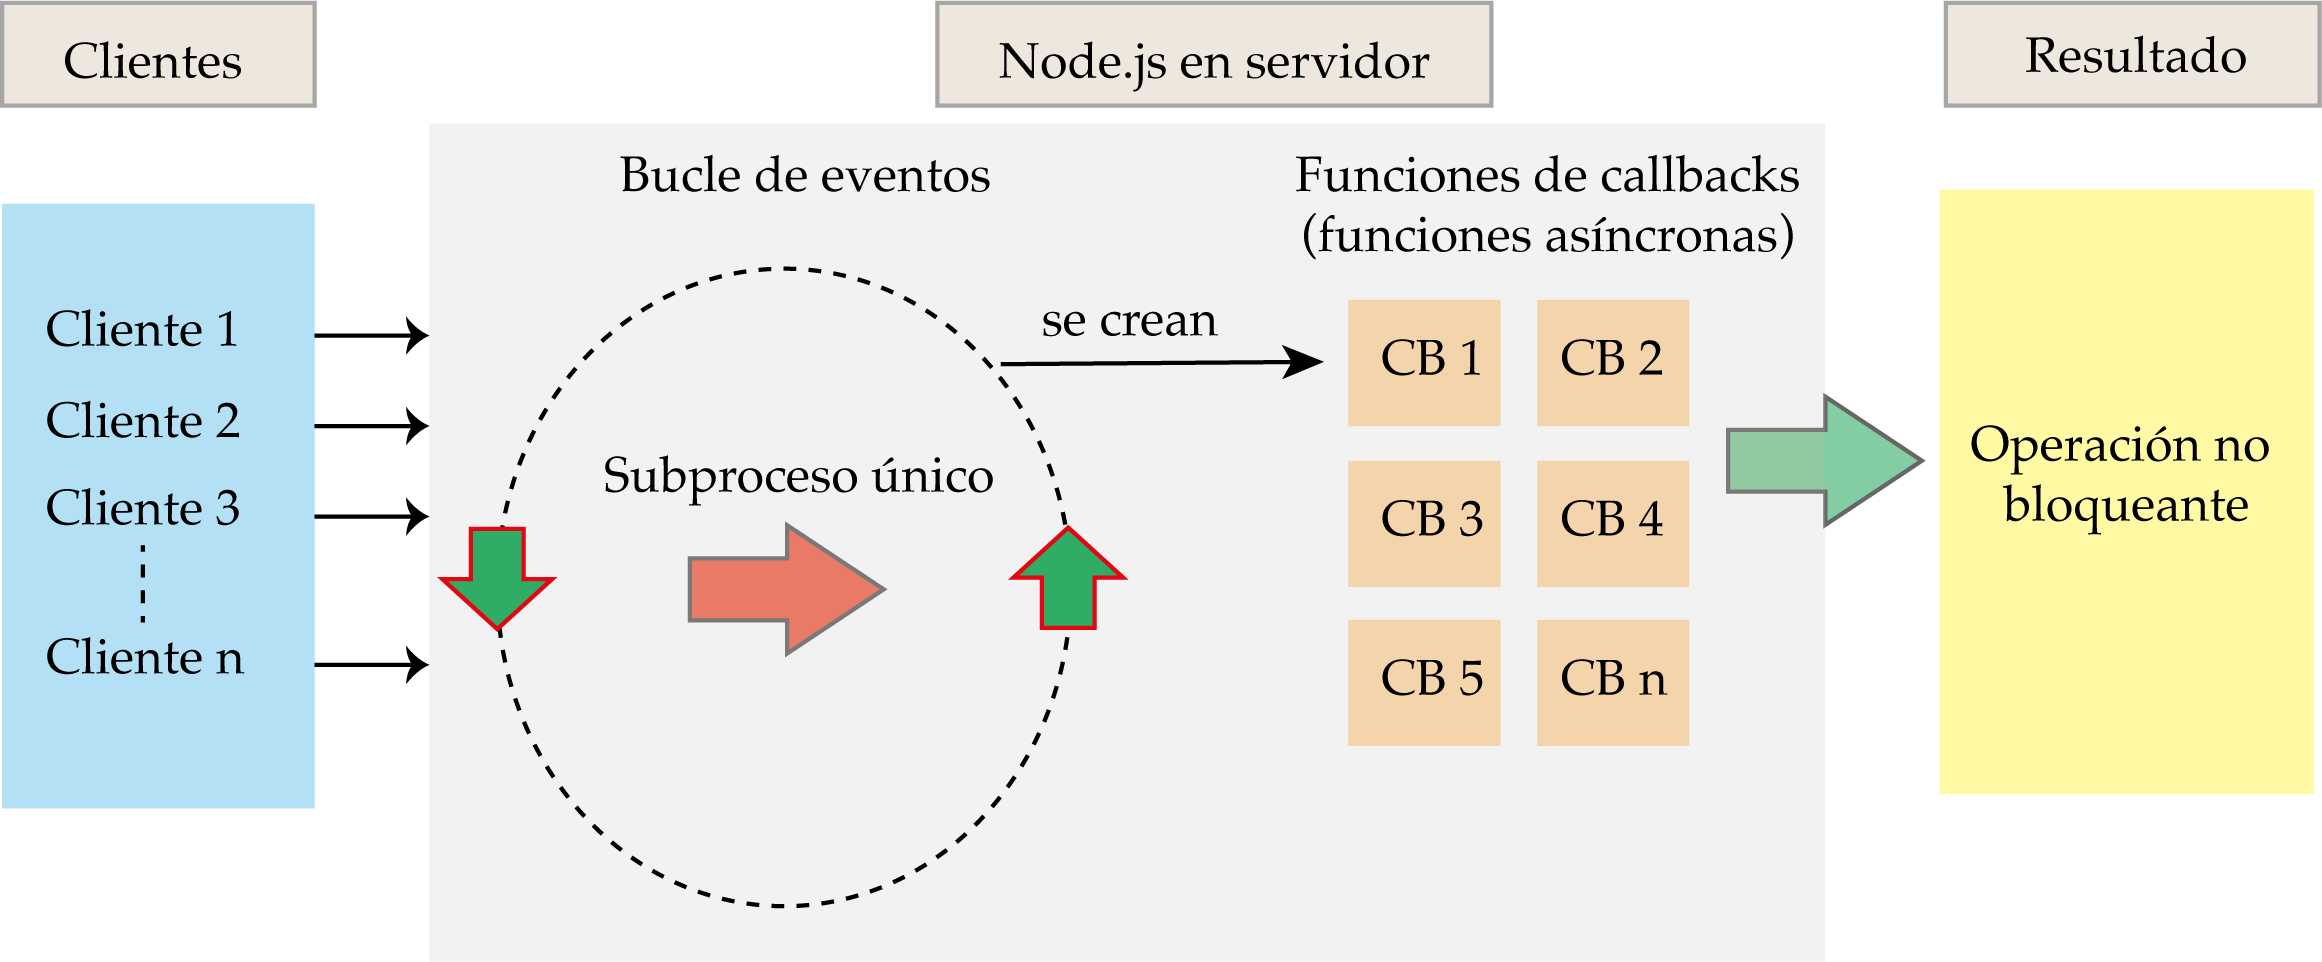
\includegraphics[scale=.65]{./Figures/node-esquema.png}
	\caption[Ejecución de Node.js en servidor ]{Ilustración del proceso de ejecución que realiza Node.js en un servidor.}
	\label{fig:node-esquema}
\end{figure}

Cuando un sistema síncrono ejecuta una llamada, las instrucciones posteriores a esa llamada no se ejecutan hasta que esta ha sido completada. Node.js es un sistema asíncrono. Esto significa que las llamadas y métodos son
ejecutados de forma secuencial, pero sin esperar a que la anterior llamada haya finalizado como se muestra en la figura \ref{fig:sinc-async}. Como conclusión podemos observar que se reduce considerablemente el tiempo de ejecución.

\begin{figure}[htpb]
	\centering
	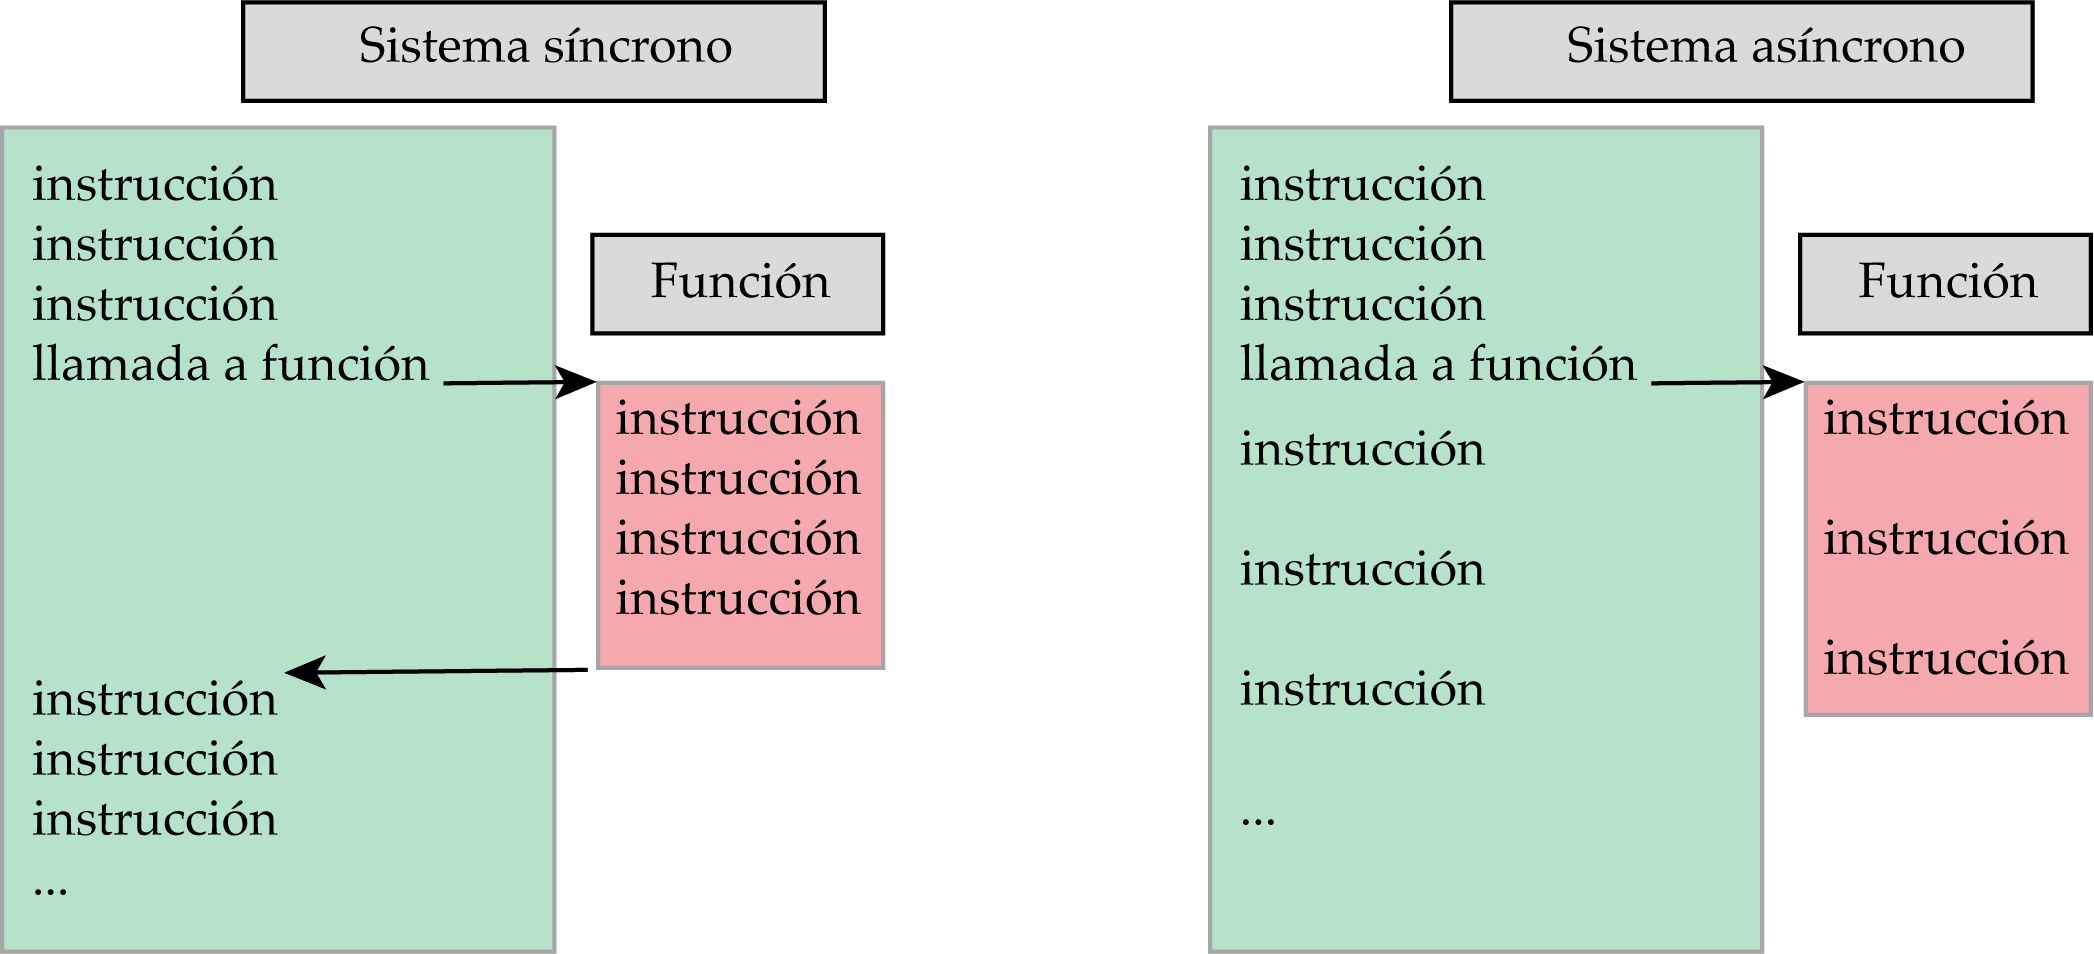
\includegraphics[scale=.65]{./Figures/funciones-asinc.png}
	\caption[Funciones síncronas y asíncronas ]{Ilustración de un sistema síncrono y un sistema asíncrono.}
	\label{fig:sinc-async}
\end{figure}


%----------------------------------------------------------------------------------------
%	SECTION {Mongo}
%----------------------------------------------------------------------------------------
\subsection{Base de datos MongoDB}

MongoDB es una base de datos noSQL \citep{WEBSITE:22},  donde se puede agregar información en forma de documentos en vez de registros como es el caso de las bases de datos SQL \citep{WEBSITE:23}.  La principal ventaja de esta base de datos noSQL es la velocidad de consulta, el motivo de esto es porque la información se la almacena en archivos de formato BSON que son versiones modificadas de JSON. 

Las características principales de MongoDB son:

\begin{itemize}
	\item Escalabilidad horizontal: MongoDB está diseñado para escalar de manera ilimitada a lo que otras bases de datos no podrían, a través de su replicación \citep{WEBSITE:24} y su \textit{sharding} \citep{WEBSITE:25} se puede almacenar información de varios equipos conectados entre sí.
	
	\item Consultas Ad hoc: permite la consulta de información a través de búsquedas de campos,
expresiones regulares con comandos de manera rápida y eficaz.

	\item Indexación: MongoDB utiliza indexación para aumentar la eficiencia en la búsqueda de
información.

	\item Replicación: MongoDB puede realizar replicación maestro – esclavo. El maestro ejecuta comandos para la lectura y escritura de los datos mientras que el esclavo realiza solo lectura de datos pero no los puede modificar.
	
	\item Distribución de carga: MongoDB permite que pueda ejecutarse en distintos servidores a la vez, haciendo más fácil su distribución en la carga de usuarios que deseen conectarse así como acceder a la información. 
	
\end{itemize}




Algunos comandos para el manejo de MongoDB se pueden observar en la tabla \ref{tab:mongo-commands}.  Normalmente en las bases de datos, se mencionan operaciones CRUD,  del acrónimo de Crear, Leer, Actualizar y Borrar (del original en ingles \textit{Create}, \textit{Read}, \textit{Insert} y \textit{Delete}) y se usa para referirse a las funciones básicas para el manejo de la información. Para el caso de MongoDB,  estas palabras se reemplazan por \textit{Insert}, \textit{Find}, \textit{Update} y \textit{Remove} respectivamente.

\begin{table}[h]
	\centering
	\caption[Comandos utilizados en MongoDB]{Comandos más utilizados para el manejo de base de datos que utiliza MongoDB.}
	\begin{tabular}{l l }    
		\toprule
		\textbf{Comando} 	 & \textbf{Descripción} 		\\
		\midrule
	
		\textit{use} 							& Crear una nueva base de dato o utilizar una existente.\\		
		\textit{insertOne}					& Crear un documento en una colección determinada.\\	
		\textit{count}						& Cuenta la cantidad de documentos que hay en una colección.\\	
		\textit{drop}							& Elimina una colección de la base de datos.\\	
		\textit{find	} 						& Se busca un documento en una colección\\
		\textit{remove}	 					& Elimina un documento de una colección\\
		\textit{update}						& Modifica un documento de una colección\\
		
		\bottomrule
		\hline
	\end{tabular}
	\label{tab:mongo-commands}
\end{table}

MongoDB almacena los documentos creados en colecciones que son el análogo a tablas en base de datos relacionales.  En la figura \ref{fig:tabla-coleccion} se ejemplifica la analogía entre tablas en base de datos relacionales y colecciones en MongoDB.

\begin{figure}[htpb]
	\centering
	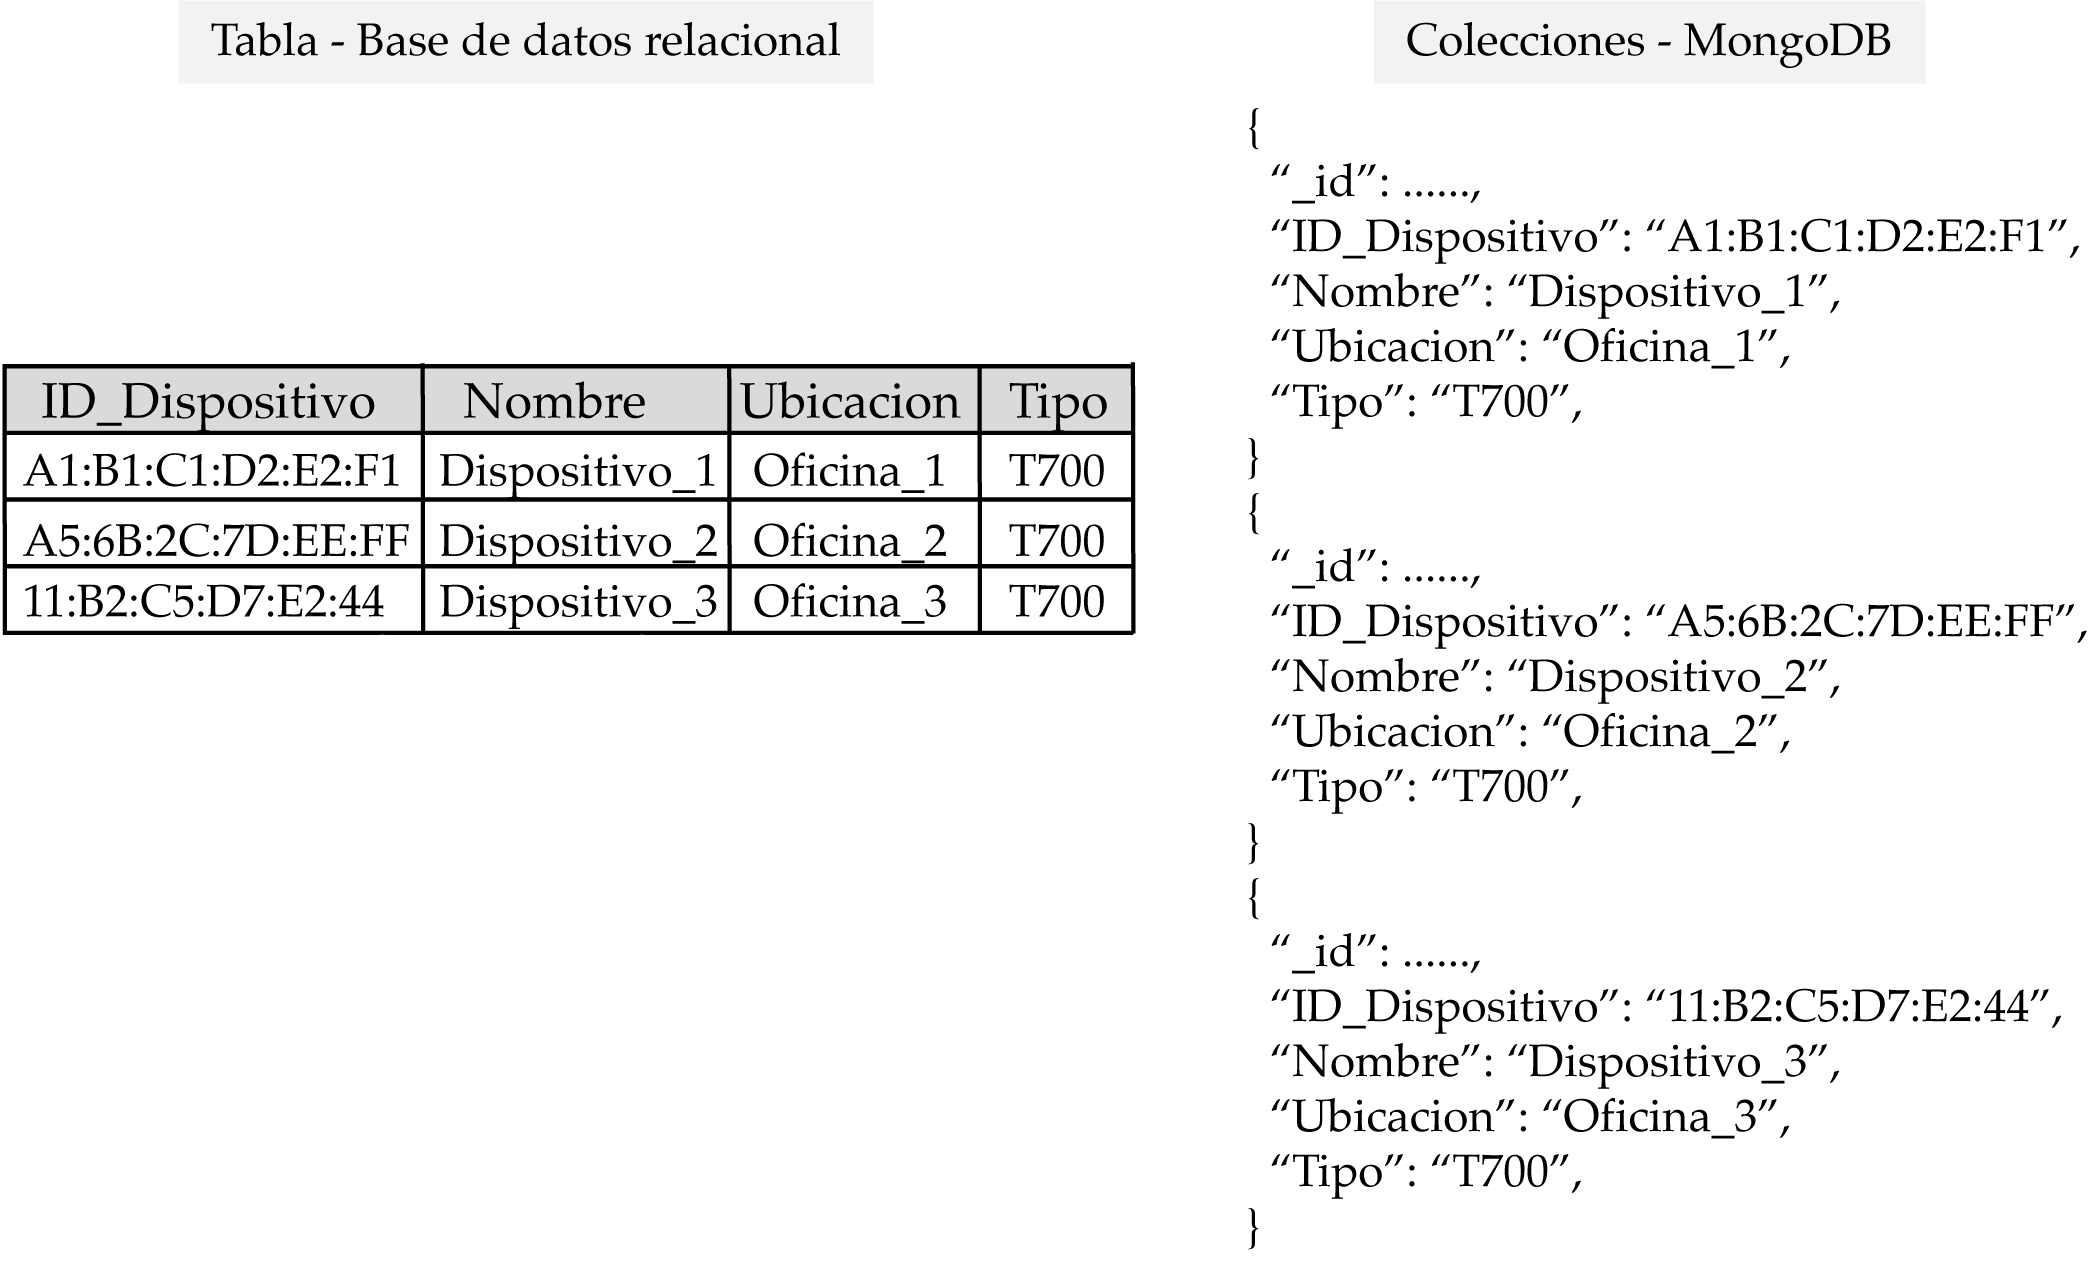
\includegraphics[scale=.75]{./Figures/tabla-coleccion.png}
	\caption[Comparación tabla - colecciones en MongoDB ]{Ilustración de analogía entre tablas en base de datos relacionales y colecciones en MongoDB.}
	\label{fig:tabla-coleccion}
\end{figure}




%----------------------------------------------------------------------------------------
%	SECTION {FrontEnd}
%----------------------------------------------------------------------------------------
\section{Infraestructura del frontend}

Frontend es la parte de un programa o dispositivo a la que un usuario puede acceder directamente. Son todas las tecnologías de diseño y desarrollo web que se ejecutan en el navegador y que se encargan de la interacción con los usuarios.  Se desarrolla, principalmente, a través de tres lenguajes: HTML (\textit{HyperText Markup Language}), CSS (\textit{Cascading Style Sheets}) \citep{WEBSITE:26} y JS (Javascript) \citep{WEBSITE:27} . Cada uno de estos lenguajes se usa para desarrollar diferentes partes del frontend.  Estos lenguajes de programación se dividen en tres tareas básicas del desarrollo:

\begin{itemize}
	\item Arquitectura: HTML es el componente más importante de cualquier proceso de desarrollo de sitios web y proporciona un marco general de cómo se verá el mismo. Es un lenguaje de marcado que nos permite indicar la estructura de nuestro documento mediante etiquetas. Este lenguaje ofrece una gran adaptabilidad, una estructuración lógica y es fácil de interpretar tanto por humanos como por máquinas.
	
	\item Apariencia : CSS (en español Hoja de Estilos en Cascada) controla el aspecto de presentación del sitio, una vez que este ya está construido con HTML.  Es un lenguaje de diseño gráfico para definir y crear la presentación de un documento estructurado escrito en un lenguaje de marcado. Está diseñado principalmente para marcar la separación del contenido del documento y la forma de presentación de este.
	
	\item Interacción: JS.  Es un lenguaje de programación basado en eventos que se utiliza para transformar una página estática en una interfaz dinámica interactuando con el usuario, el navegador y el servidor.  JavaScript es un lenguaje de programación interpretado, dialecto del estándar ECMAScript \citep{WEBSITE:28}.  Se define como orientado a objetos, basado en prototipos, imperativo, débilmente tipado y dinámico.
	
\end{itemize}

Para el desarrollo del frontend de este trabajo se utilizó Angular \citep{WEBSITE:29} que es un \textit{framework} de diseño eficiente y sofisticado de plataformas web. 

%----------------------------------------------------------------------------------------
%	SECTION {Angular}
%----------------------------------------------------------------------------------------
\subsection{Angular}

Angular es una plataforma de desarrollo construida sobre \textit{Typescript} \citep{WEBSITE:30}. Como plataforma, Angular incluye:

\begin{itemize}
	\item Un marco basado en componentes para crear aplicaciones web escalables.
	
	\item Una colección de bibliotecas bien integradas que cubren una amplia variedad de características, que incluyen enrutamiento, administración de formularios, comunicación cliente-servidor, entre otras.
	
	\item Un conjunto de herramientas para desarrolladores que ayudan a desarrollar, compilar, probar y actualizar el código.
	
\end{itemize}

Para crear aplicaciones con Angular, se generan \textit{templates} con HTML y se controlan estos mismos con lógica creada en los componentes, que serán exportados como clases. Así mismo, se agrega lógica en servicios para manejar datos que la aplicación tendrá y finalmente se encapsulan los componentes y servicios en módulos o \textit{NgModules}.

Cuando se inicia la aplicación, lo hace desde el \textit{root module}. Angular toma el control y muestra el contenido en el explorador web, reaccionando a la interacción de los usuarios que utilicen la aplicación de acuerdo a las instrucciones que contiene la lógica programada.

Un módulo o \textit{NgModule} declara un contexto de compilación para un conjunto de componentes. Puede asociar sus componentes con servicios, para formar unidades funcionales. 

Cada aplicación generada con Angular cuenta con un \textit{root module} o módulo de raíz llamado convencionalmente \textit{AppModule}, el cual provee el mecanismo de arranque que inicia la aplicación. Una aplicación contiene varios módulos funcionales, además, un módulo puede importar funcionalidades de otros módulos, y exportar sus propias funcionalidades. 

Cada aplicación de Angular tiene al menos un componente. Al igual que el \textit{root module}, existe el \textit{root component} que conecta una jerarquía de componentes con el DOM (\textit{Document Object Model}) \citep{WEBSITE:31}.  Cada componente define una clase que contiene datos y lógica, y está vinculada con el archivo HTML.

El binding a propiedades, o \textit{property binding} en inglés, sirve para asignar un valor a una propiedad de un elemento de un \textit{template}. Esa asignación podrá ser un valor literal, escrito tal cual en el \textit{template}, pero generalmente se tratará de un valor obtenido a través de una propiedad del componente, de modo que si el estado del componente cambia, también cambia la propiedad del elemento asignada en el template.

Por otro lado, cuando un usuario interactúa con un enlace, pulsa un botón, selecciona un evento de una lista desplegable o manipula el texto, el binding de eventos o \textit{event binding} permite a una aplicación de Angular ejecutar código y acciones cuando se produce un evento.

Todos los datos o lógica que no está asociada directamente a una vista y que requiera ser utilizada en diferentes partes de la aplicación y entre diferentes componentes, puede ser escrita en un servicio. Al igual que un componente, los servicios son exportados como clases. Los servicios cuentan con el decorador @Injectable() que provee metadata que permite que los servicios sean inyectados en componentes como dependencias.  \textit{Dependency injection} o Inyección de Dependencias permite manejar las clases de los componentes de forma ligera y eficiente. 

El esquema de la figura \ref{fig:esquema-angular} ejemplifica en forma de bloques, el funcionamiento general de Angular.

\begin{figure}[htpb]
	\centering
	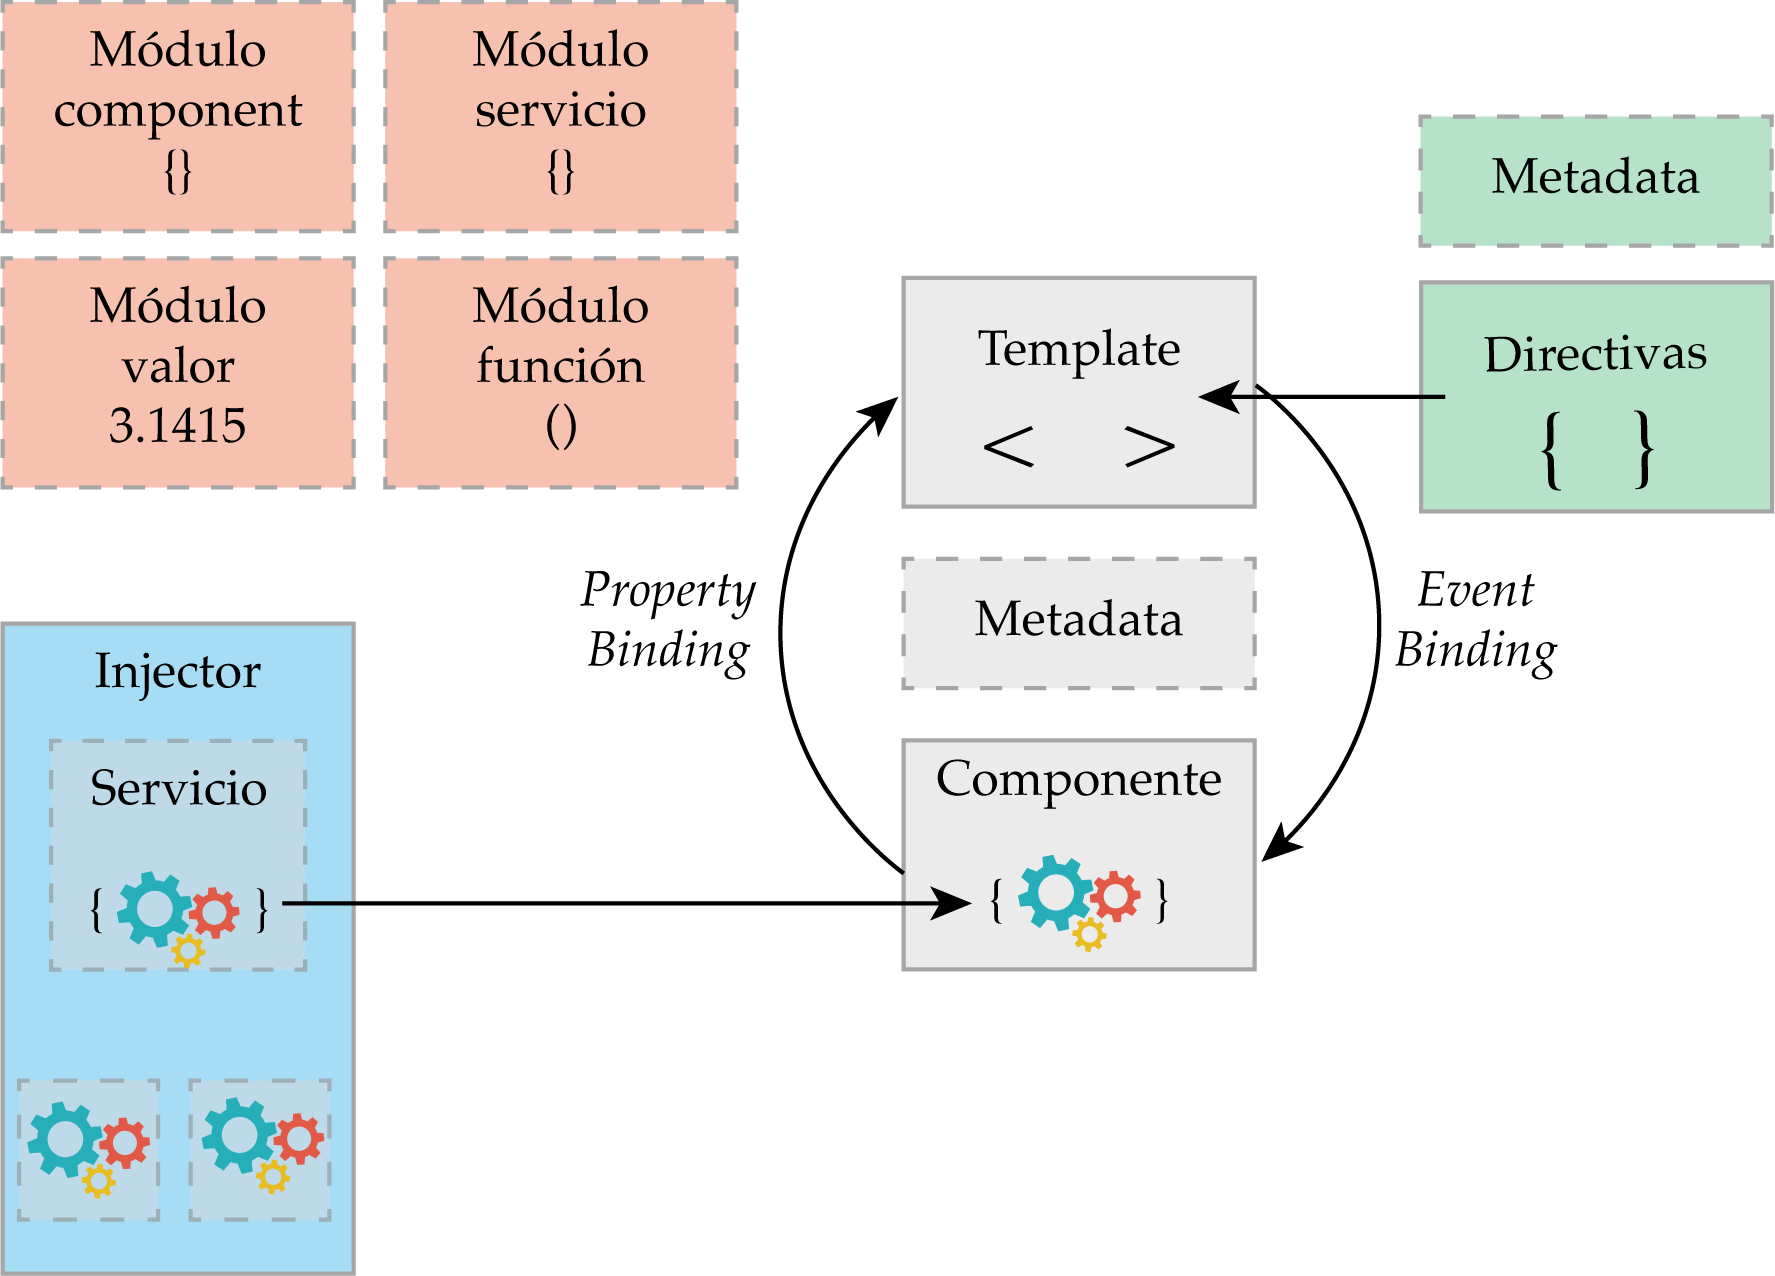
\includegraphics[scale=.7]{./Figures/angular-esquema.png}
	\caption[Arquitectura de funcionamiento de Angular ]{Ilustración de arquitectura de funcionamiento de Angular\protect\footnotemark.}
	\label{fig:esquema-angular}
\end{figure}

\footnotetext{Imagen acondicionada de \url{https://angular.io/guide/architecture}}
%----------------------------------------------------------------------------------------
%	SECTION {Nginx}
%----------------------------------------------------------------------------------------
\section{Servidor Nginx}


Nginx \citep{WEBSITE:32} es un servidor web de código abierto que también es usado como proxy inverso, cache de HTTP, y balanceador de carga.  Es un software modular, lo que significa que las diferentes características son presentadas en forma de módulos, y como administrador, pueden ser activadas o desactivadas. Como consecuencia, el usuario goza de las siguientes características:

\begin{itemize}
	\item \textit{Application Acceleration} (acelerador de aplicaciones), agiliza la entrega de contenidos.
	
	\item Servidor proxy inverso para la aceleración web (HTTP, TCP, UDP) o como proxy de correo electrónico (IMAP, POP3, SMTP).
	
	\item Cifrado TLS para una transferencia de datos segura.
	
	\item Gestión de ancho de banda para un mejor rendimiento.
	
	\item Balanceo de carga con reorientación de solicitudes para disminuir la carga del servidor.
	
\end{itemize}


Nginx trabaja enfocado a eventos. Como consecuencia, puede procesar solicitudes de forma asíncrona, ahorrando memoria y espacio. Este software de servidor es soportado por una gran variedad de sistemas operativos, incluyendo variantes de UNIX / Linux, Mac OS o Windows, fue concebido inicialmente como una respuesta al problema C10K \citep{WEBSITE:33}, que se refiere al problema de rendimiento de manejar 10,000 conexiones concurrentes.

Logra excelentes resultados en el procesamiento de un gran número de solicitudes de los clientes y aprovecha eficazmente los recursos.

Nginx es un servidor asíncrono construido buscando solucionar los problemas de concurrencia que experimentaban ciertos sitios. El algoritmo desarrollado para este servidor es mucho más eficiente y consume menos recursos.

Nginx genera procesos \textit{worker}, cada uno de los cuales puede manejar muchas conexiones. Se puede lograr esto debido a la implementación de un mecanismo de bucle rápido que busca y procesa eventos continuamente. Cada conexión manejada por el \textit{worker} es dispuesta dentro del bucle de eventos, donde vive con otras conexiones. Los eventos dentro de este bucle se procesan de forma asíncrona, permitiendo que el trabajo sea manejado de forma no bloqueante. Cuando una conexión se cierra, se elimina del bucle. Esta disposición asíncrona y monohilos ayuda a que, incluso con recursos limitados, Nginx sea bastante rápido en cuanto al procesamiento de conexiones. Por consiguiente, el uso de CPU y memoria tiende a bajar debido a la eficiencia en el manejo de conexiones. En la figura  \ref{fig:worker-nginx} se ejemplifica el proceso principal de Nginx con la creación de n \textit{workers} por cada consulta / respuesta.

\begin{figure}[htpb]
	\centering
	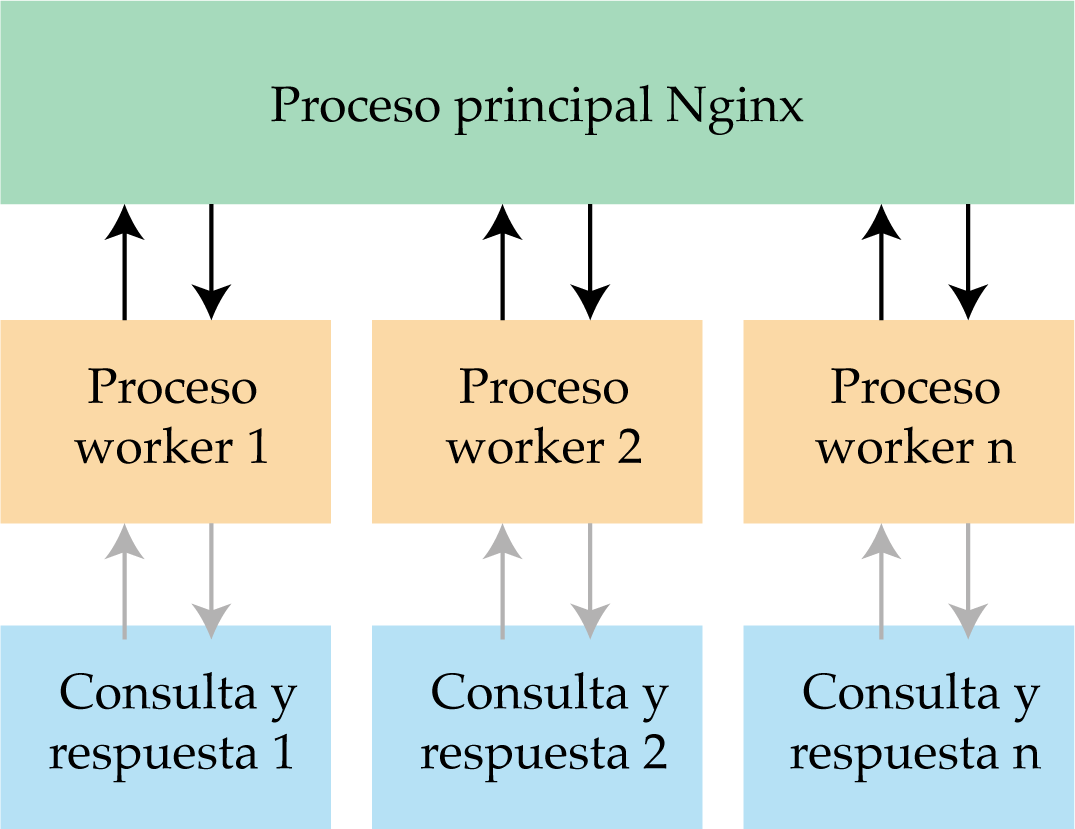
\includegraphics[scale=.7]{./Figures/worker-nginx.png}
	\caption[Proceso principal Nginx ]{Ilustración de funcionamiento principal de Nginx con n consultas / respuestas.}
	\label{fig:worker-nginx}
\end{figure}

Para este trabajo se utilizó Nginx como proxy inverso. Se conoce como proxy inverso cuando un servidor acepta todo el tráfico y lo reenvía a un recurso específico, por ejemplo a una consulta al backend o bien acceder al frontend. El motivo para utilizar un servidor proxy inverso es el agregado de seguridad al servidor principal,  restringir el acceso a rutas definidas y evitar ataques. En la figura \ref{fig:proxy-nginx}  se observa la configuración típica de Nginx como proxy inverso, donde se destaca que cada uno de los clientes tendrán un solo punto de acceso a los recursos del servidor. 

\begin{figure}[htpb]
	\centering
	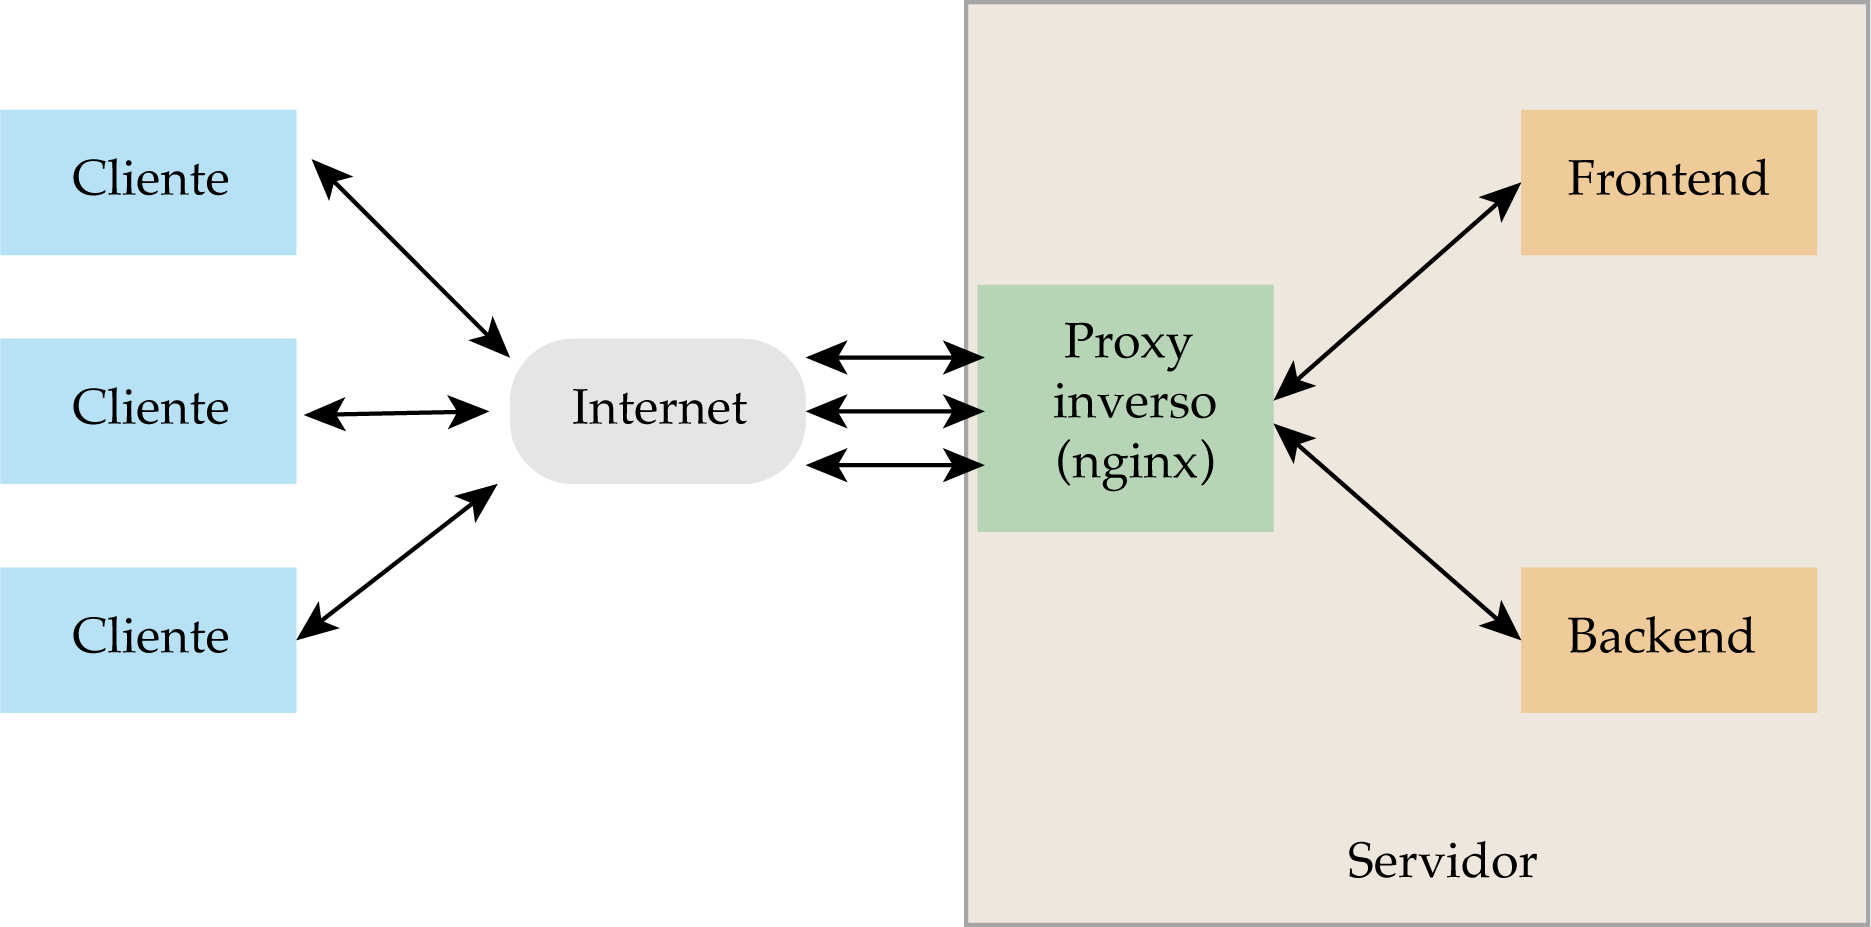
\includegraphics[scale=.7]{./Figures/ngix-proxy.png}
	\caption[Configuración Nginx como proxy inverso ]{Ilustración de configuración de ngix como proxy inverso.}
	\label{fig:proxy-nginx}
\end{figure}



















 
\chapter{Diseño e implementación} % Main chapter title

\label{Chapter3} % Change X to a consecutive number; for referencing this chapter elsewhere, use \ref{ChapterX}

\definecolor{mygreen}{rgb}{0,0.6,0}
\definecolor{mygray}{rgb}{0.5,0.5,0.5}
\definecolor{mymauve}{rgb}{0.58,0,0.82}

%%%%%%%%%%%%%%%%%%%%%%%%%%%%%%%%%%%%%%%%%%%%%%%%%%%%%%%%%%%%%%%%%%%%%%%%%%%%%
% parámetros para configurar el formato del código en los entornos lstlisting
%%%%%%%%%%%%%%%%%%%%%%%%%%%%%%%%%%%%%%%%%%%%%%%%%%%%%%%%%%%%%%%%%%%%%%%%%%%%%
\lstset{ %
  backgroundcolor=\color{white},   % choose the background color; you must add \usepackage{color} or \usepackage{xcolor}
  basicstyle=\footnotesize,        % the size of the fonts that are used for the code
  breakatwhitespace=false,         % sets if automatic breaks should only happen at whitespace
  breaklines=true,                 % sets automatic line breaking
  captionpos=b,                    % sets the caption-position to bottom
  commentstyle=\color{mygreen},    % comment style
  deletekeywords={...},            % if you want to delete keywords from the given language
  %escapeinside={\%*}{*)},          % if you want to add LaTeX within your code
  %extendedchars=true,              % lets you use non-ASCII characters; for 8-bits encodings only, does not work with UTF-8
  %frame=single,	                % adds a frame around the code
  keepspaces=true,                 % keeps spaces in text, useful for keeping indentation of code (possibly needs columns=flexible)
  keywordstyle=\color{blue},       % keyword style
  language=[ANSI]C,                % the language of the code
  %otherkeywords={*,...},           % if you want to add more keywords to the set
  numbers=left,                    % where to put the line-numbers; possible values are (none, left, right)
  numbersep=5pt,                   % how far the line-numbers are from the code
  numberstyle=\tiny\color{mygray}, % the style that is used for the line-numbers
  rulecolor=\color{black},         % if not set, the frame-color may be changed on line-breaks within not-black text (e.g. comments (green here))
  showspaces=false,                % show spaces everywhere adding particular underscores; it overrides 'showstringspaces'
  showstringspaces=false,          % underline spaces within strings only
  showtabs=false,                  % show tabs within strings adding particular underscores
  stepnumber=1,                    % the step between two line-numbers. If it's 1, each line will be numbered
  stringstyle=\color{mymauve},     % string literal style
  tabsize=2,	                   % sets default tabsize to 2 spaces
  title=\lstname,                  % show the filename of files included with \lstinputlisting; also try caption instead of title
  morecomment=[s]{/*}{*/}
}

En este capítulo se detalla el diseño de la arquitectura del sistema en todos sus componentes. Se menciona el motivo de elección en cada caso y la implementación correspondiente.

%----------------------------------------------------------------------------------------
%	SECTION 1
%----------------------------------------------------------------------------------------
\section{Diseño de la estructura general del sistema}
\label{seccion-intro}
La estructura del sistema implementado puede observarse en la figura \ref{fig:esquema-general}. El sistema consta de clientes que serán navegadores web para acceder al frontend y a las API \citep{WEBSITE:34} que contiene el backend. Por otro lado, del lado del cliente, los dispositivos conversores Modbus a MQTT se conectan al broker que también forma parte del servidor.

Las funciones implementadas en el backend se conectan a una base de datos remota para almacenar los datos de clientes web o bien mediciones de dispositivos conectados.

\begin{figure}[htpb]
	\centering
	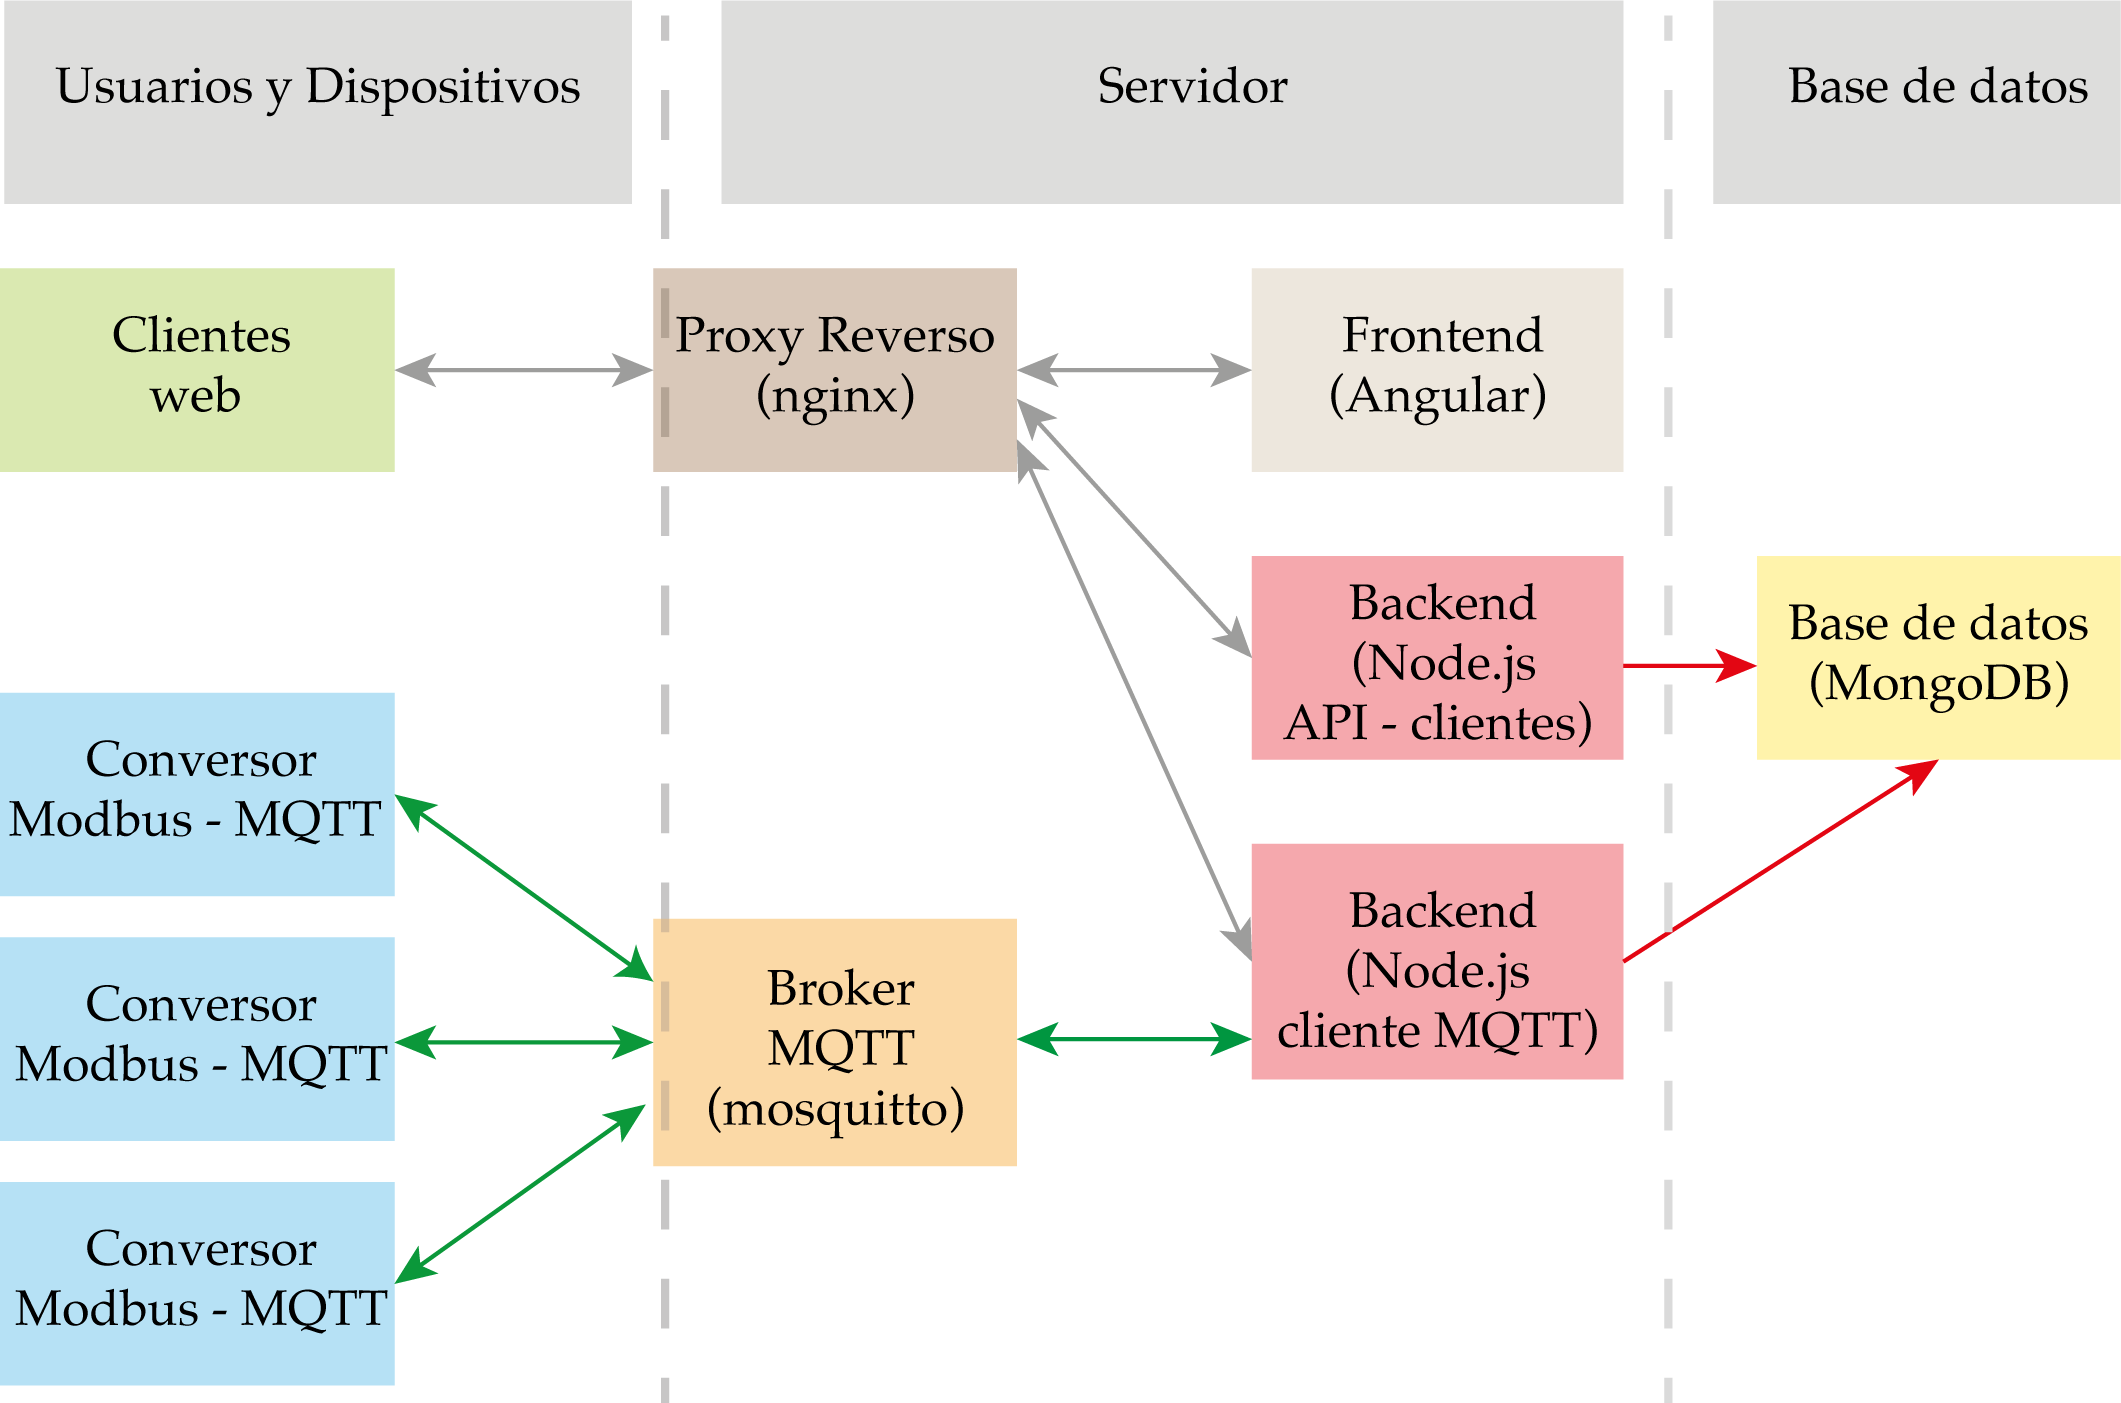
\includegraphics[scale=.75]{./Figures/esquema-general.png}
	\caption[Diagrama de bloques de sistema implementado ]{Diagrama de bloques de sistema de gestión implementado.}
	\label{fig:esquema-general}
\end{figure}
 
En el servidor se desarrolló el frontend en Angular mientras que el backend consta de dos módulos. Por un lado el modulo de API de clientes que fue desarrollado en Node.js y contiene la implementación de funciones para interactuar con la base de datos y la creación de usuarios, dispositivos y visualización de configuración.  Además el backend consta de un módulo cliente MQTT que se encarga de interactuar entre el broker y los dispositivos conectados a él. Es el encargado de gestionar la información que envían los dispositivos hacia la base de datos para luego ser utilizados por el frontend. 

Todo el servidor es gestionado por Nginx, el cual actúa como proxy inverso lo que permite un único canal de comunicación entre usuarios y sistema.  Por último, la base de datos se encuentra en un servidor remoto y se accede a ella mediante credenciales de conexión. 
 
 
\section{Implementación del backend}
\label{backend-sec}
El backend del trabajo realizado está divido en diferentes bloques de funcionamiento. 

El bloque de backend de funciones API de clientes que se observa en la figura \ref{fig:backend-clientes} donde su conexión con el punto de entrada al servidor gestionado por Nginx es el puerto 8000.  Por otro lado, este bloque se conecta con la base de datos remota MongoDB Atlas \citep{WEBSITE:35} para almacenar datos de nuevos usuarios, dispositivos,configuración de dispositivos, organizaciones y relaciones entre usuarios y organizaciones.  Los clientes que acceden a cualquier función de este bloque lo harán a través de un puerto seguro, dotado de certificados SSL que es manejado por Nginx y mapeado al puerto 8000.

\begin{figure}[htpb]
	\centering
	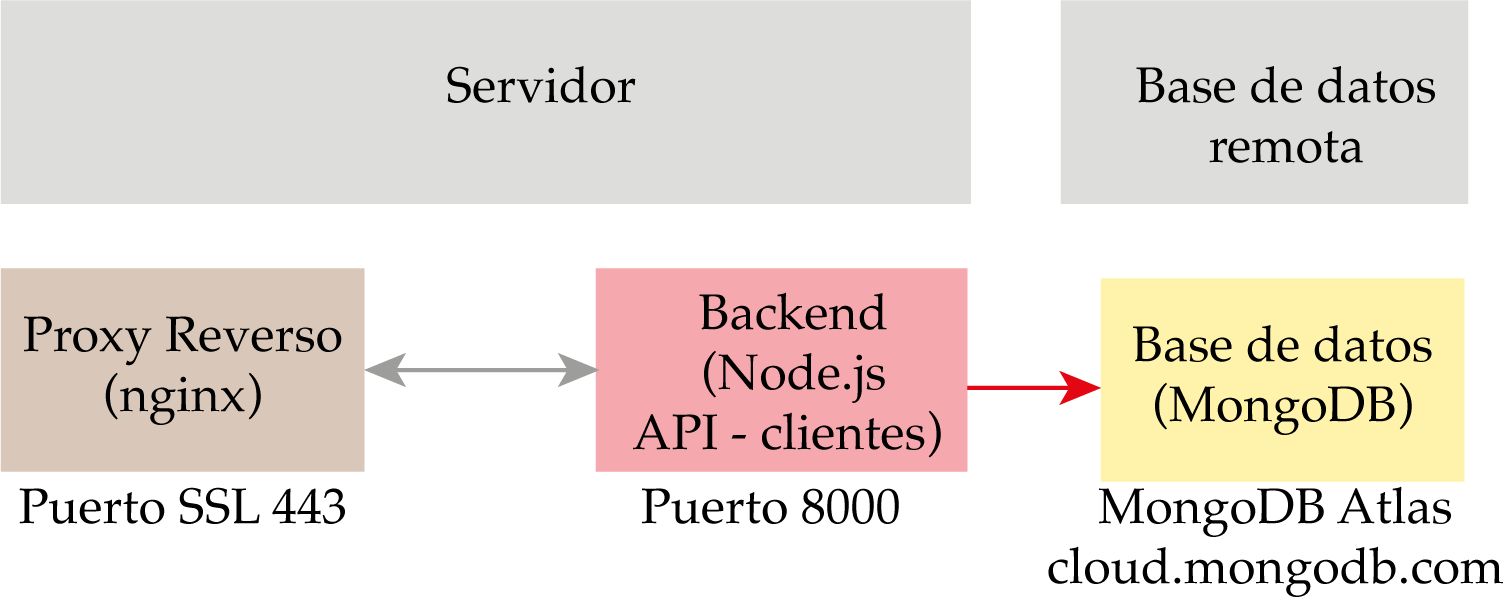
\includegraphics[scale=.75]{./Figures/backend-clientes.png}
	\caption[Conexión entre Nginx - API clientes y base de datos]{Diagrama de conexión entre Nginx, modulo de API de clientes y base de datos en MongoDB Atlas.}
	\label{fig:backend-clientes}
\end{figure}

La estructura interna de este bloque consta de rutas y un bloque de funciones para el manejo antes mencionado. En la figura \ref{fig:bloque-api-clientes} puede observarse un desglose general de este bloque. 

\begin{figure}[htpb]
	\centering
	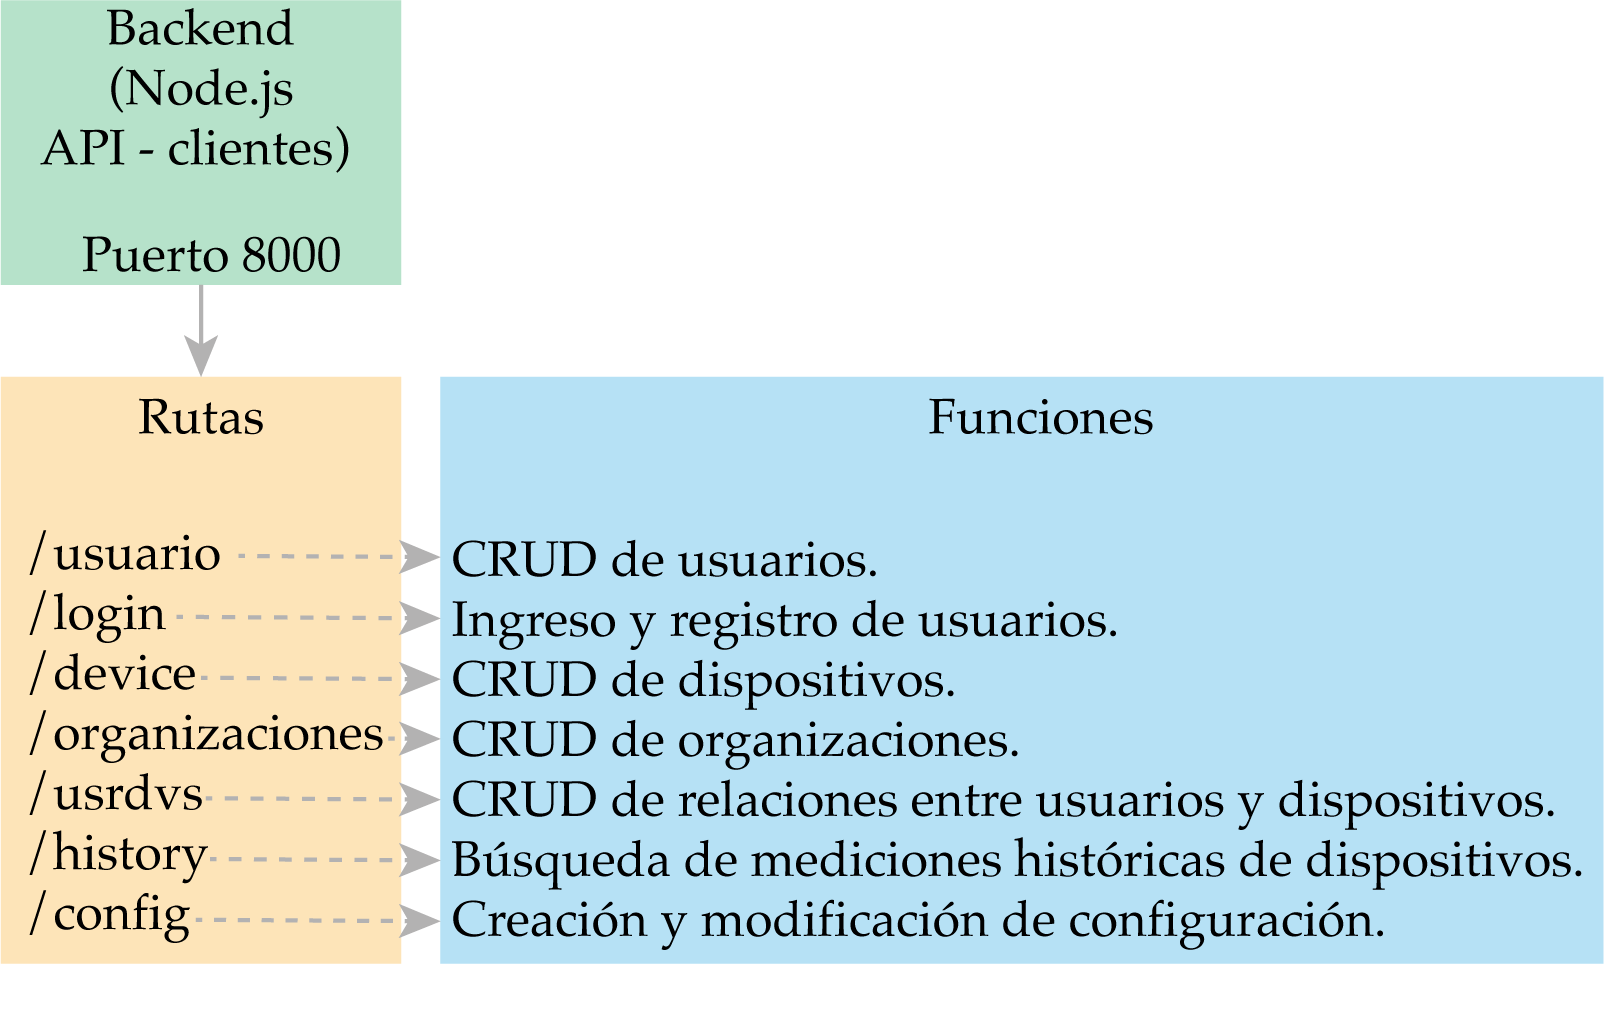
\includegraphics[scale=.75]{./Figures/bloque-api-clientes.png}
	\caption[Descripción bloque API clientes]{Descripción de rutas y funciones principales de bloque API clientes.}
	\label{fig:bloque-api-clientes}
\end{figure}

Se utilizó la librería de Node.js llamada Express.js \citep{WEBSITE:36} la cual proporciona mecanismos para:

\begin{itemize}
	\item Escritura de manejadores de peticiones con diferentes verbos HTTP en diferentes rutas.
	
	\item Integración con motores de renderización de vistas para generar respuestas mediante la introducción de datos en plantillas.
	
	\item Establecer ajustes de aplicaciones web como qué puerto usar para conectar, y la localización de las plantillas que se utilizan para renderizar la respuesta.

	\item Añadir procesamiento de peticiones \textit{middleware} adicional en cualquier punto dentro de la tubería de manejo de la petición.

\end{itemize}

En el código \ref{cod:express-code} se muestra la forma adoptada para crear las rutas para las funciones de gestión.

\begin{lstlisting}[label=cod:express-code,caption=Utilización de Express para crear rutas en el servidor.] 

// Inclusion del modulo express

var express = require('express');

var app = express();

//Rutas 
app.use('/usuario', require('./routes/usuario'));

app.use('/login', require('./routes/auth'));

app.use('/device', require('./routes/devices'));

app.use('/organizaciones', require('./routes/organizations'));

app.use('/usrdvs', require('./routes/usrs_dev'));

app.use('/history', require('./routes/historical'));

app.use('/config', require('./routes/sensors-config'));


// Escuchar peticiones
app.listen(process.env.PORT, () => {
    console.log('server: \x1b[32m%s\x1b[0m', 'running');
});

\end{lstlisting}

Otra biblioteca importante que se utiliza en este bloque es Mongoose \citep{WEBSITE:38}, que se utiliza para escribir consultas para una base de datos de MongoDB, con características como validaciones, construcción de \textit{queries, middlewares,} conversión de tipos entre otras, que enriquecen la funcionalidad de la base de datos. 

La parte central del uso de Mongoose está en la definición de un esquema donde se indica la configuración de los documentos para una colección de MongoDB.  En el código \ref{cod:mongoose-code} se muestra su inicialización y la conexión remota. 

\begin{lstlisting}[label=cod:mongoose-code,caption=Utilización de Mongoose para el manejo de MongoDB.] 

// Inclusion de mongoose.
var mongoose = require('mongoose');

// Conexion a la base de dato remota
try {
        await mongoose.connect( process.env.DB_CNN , {
            useNewUrlParser: true, 
            useUnifiedTopology: true,
            useCreateIndex: true
        });

        console.log('DB Online');
        
    } catch (error) {
        console.log(error);
        throw new Error('Error a la hora de iniciar la BD');
    }
}

\end{lstlisting}


Además, dentro del backend del trabajo realizado, se encuentra el bloque para el manejo de mensajes MQTT que se publican en el broker y provienen de los dispositivos conectados a él.  En la figura \ref{fig:backend-mqtt-server} se puede ver su conexión con el broker y además con la base de datos MongoDB. 

\begin{figure}[htpb]
	\centering
	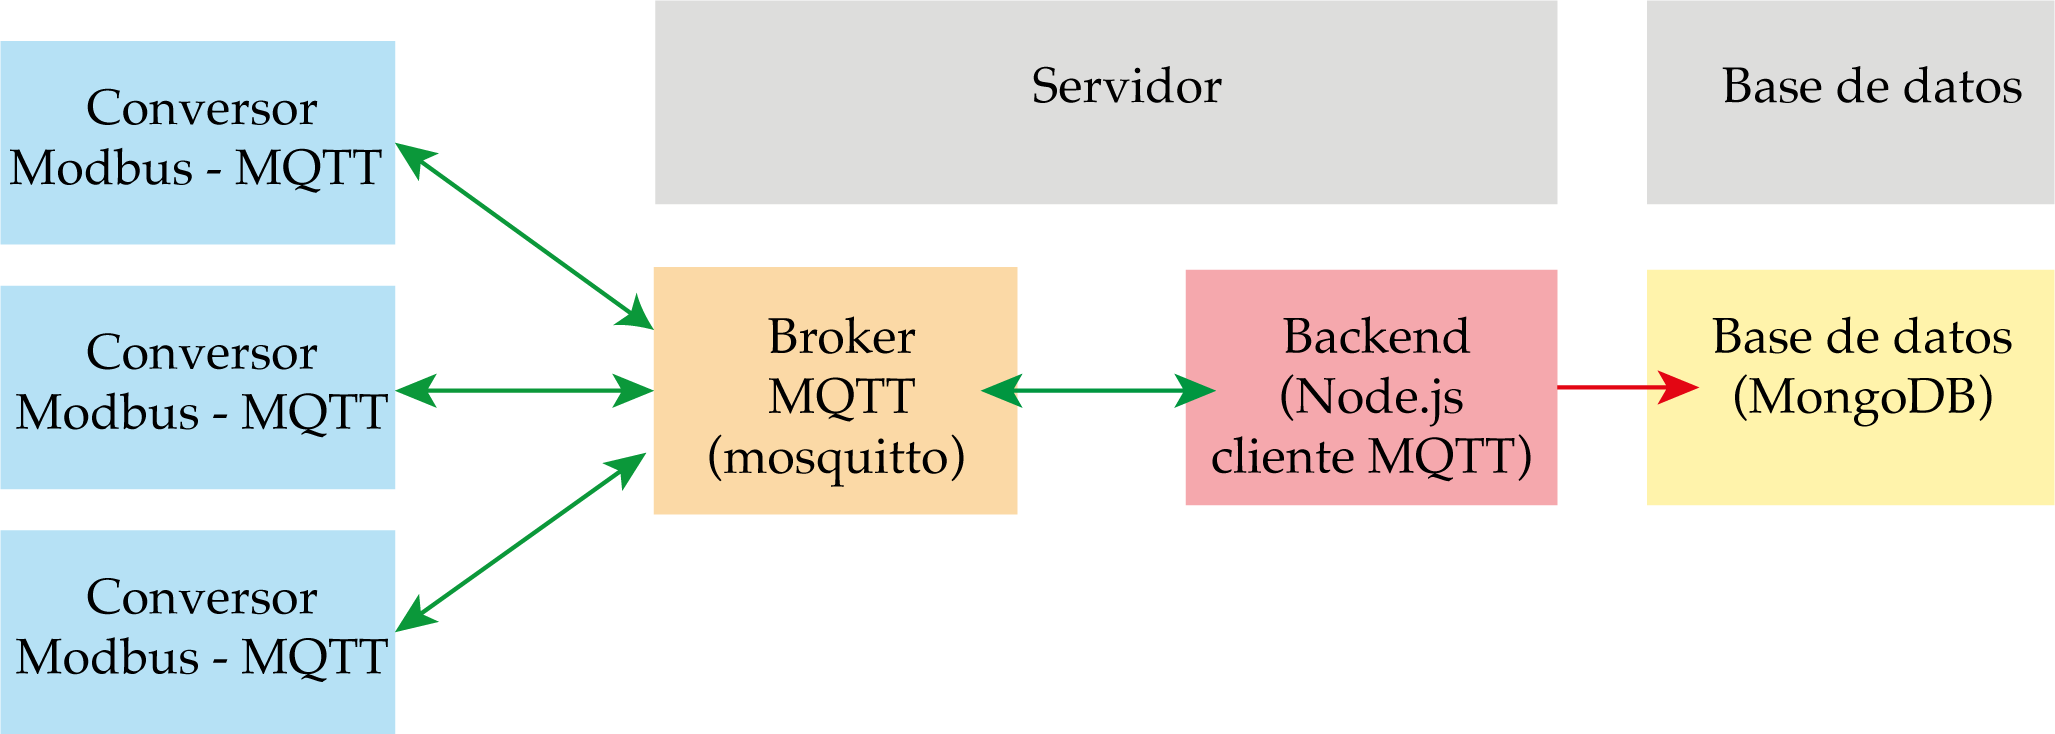
\includegraphics[scale=.75]{./Figures/backend-mqtt.png}
	\caption[Descripción bloque cliente MQTT]{Descripción de cliente MQTT implementado en el servidor.}
	\label{fig:backend-mqtt-server}
\end{figure}


Para crear un cliente MQTT en Node.js se utiliza la librería MQTT.js \citep{WEBSITE:38} con la cual se pueden crear clientes que se conecten al broker del sistema. En el código \ref{cod:mqtt-code} se muestra la implementación en el backend del servidor.

\begin{lstlisting}[label=cod:mqtt-code,caption=Cliente MQTT en el servidor utilizando librería  MQTT.js.] 

// Incluimos la libreria mqtt
var mqtt = require('mqtt');

// Definicion de variables de conexion.
var options= {
            port: +process.env.MB_PORT,
            username: process.env.MB_USERNAME,
            password: process.env.MB_PASSWORD,           
};
   
// Conexion al broker MQTT     
var client  = mqtt.connect(process.env.MB_URL, options);

/* Evento de conexion con el broker */
client.on('connect', function() {
		logger._log('info','MQTT broker conectado');

            /* Subscripcion a los topicos */
           MQTTsubscriber.subscribe(client);
});

/* Evento de error en la conexion con el broker */
client.on('error', (error) => {
        	logger._log('error','Error: ' + error.message);
            
});

/* Evento de reconexion del broker */
client.on('reconnect', () => {
		logger._log('warn','Reconectando al Broker MQTT');
});

/* Evento de conexion cerrada con el broker */
client.on('close', () => {
		logger._log('warn','Conexion con el broker cerrada');
});

/* Evento de broker Offline */
client.on('offline', () => {
		logger._log('info','Conexion con el broker Offline');
});

/* Evento de broker finalizado */
client.on('end', () => {
	 	logger._log('info','Conexion con el broker Finalizada');
});

/* Evento de mensaje del broker donde se recibe 
* el topico y el mensaje 
*/
client.on('message', function(topic, message, packet) {
	 	console.log(topic);
		console.log(message);
	 	console.log(packet);

		MQTTsubscriber.observe(topic,message,packet);
});
\end{lstlisting}


\subsection{Modelos utilizados en la base de datos}

Para el manejo de la base de datos, Mongoose requiere que se creen \textit{Schemas} de cada uno de los modelos que intervienen en este trabajo. 

Para la implementación del modelo de usuario se realizo un estudio de los campos requeridos por el cliente que requiere el registro y acceso al sistema. El código  \ref{cod:user-model}  muestra esta definición en conjunto con sentencias para validar información del modelo.

\begin{lstlisting}[label=cod:user-model,caption=Definición de Schema para el modelo de usuario.] 

// Inclusion de librerias utilizadas
var mongoose = require('mongoose');
var uniqueValidator = require('mongoose-unique-validator');

// Definicion de Schema
var Schema = mongoose.Schema;

// Variable con roles permitidos cuando se crea un usuario.
var rolesValidos = {
    values: ['CREATOR_ROLE', 'ADMIN_ROLE', 'USER_ROLE'],
    default: 'USER_ROLE',
    message: '{VALUE} no es un rol permitido'
};

//Creo el schema para el modelo de Usuario
var usuarioSchema = new Schema({

    nombre: { type: String, required: [true, 'El nombre es requerdio'] },
    email: { type: String, unique: true, required: [true, 'El correo es necesario'] },
    
    role: { type: String, 
            required: true, 
            default: 'USER_ROLE', 
            enum: rolesValidos },
    created_by: { type: Schema.Types.ObjectId, ref: 'Usuario', require:[true, 'debe crearlo un usuario'] },
    created: { type: String, default: '' },
    updated: { type: String, default: '' },
    deleted: { type: String, default: '' },
});

// Plugin que me permite enviar un mensaje de error cuando se hacen las validaciones.
usuarioSchema.plugin(uniqueValidator, { message: '{PATH} debe ser unico' });

// Exporto el modelo para que se pueda utilizar en las funciones del programa.
module.exports = mongoose.model('Usuario', usuarioSchema);

\end{lstlisting}

Para el resto de los modelos utilizados en el trabajo, el procedimiento adoptado es similar al del código \ref{cod:user-model}. En la figura \ref{fig:modelos-mongo} se muestran los modelos mas utilizados en este trabajo para realizar operaciones con la base de datos. 

\begin{figure}[htpb]
	\centering
	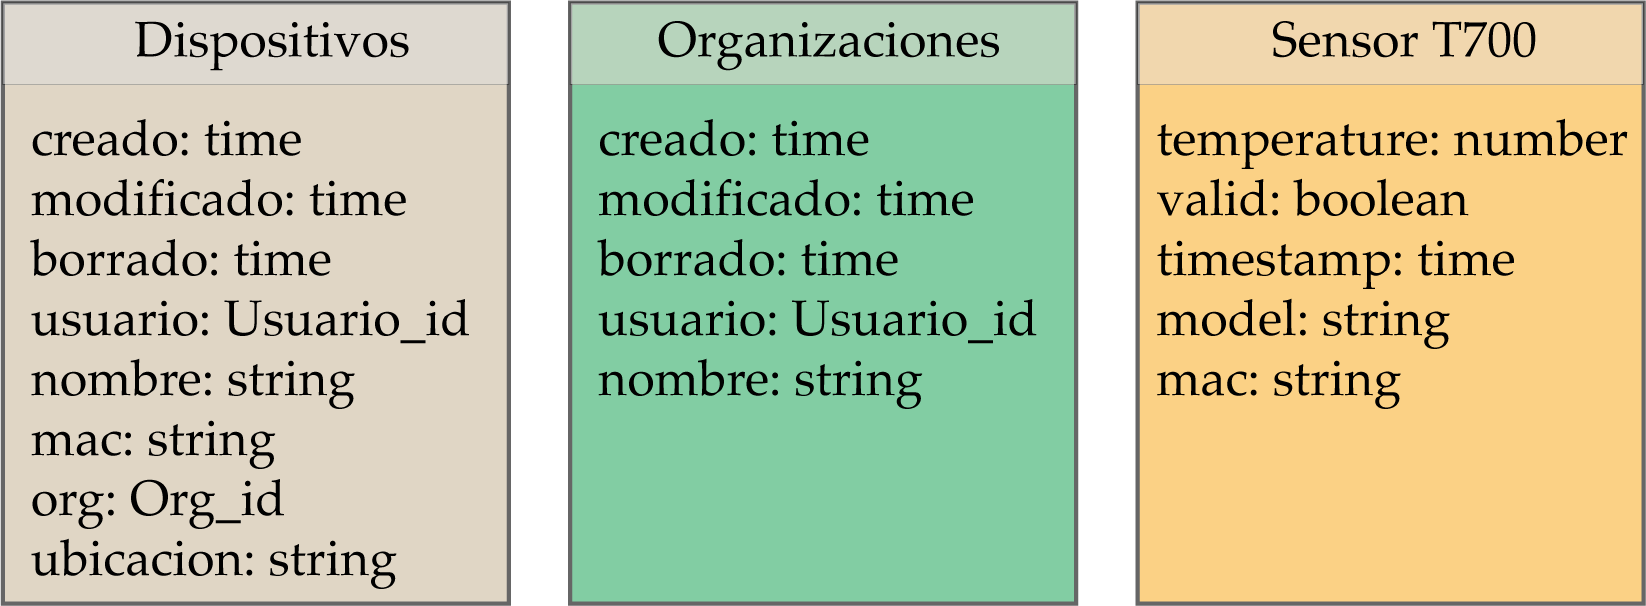
\includegraphics[scale=.75]{./Figures/modelos-mongo.png}
	\caption[Modelos de datos utilizados en Mongoose]{Descripción modelos de datos utilizados para crear los Schemas para realizar operaciones en Mongoose.}
	\label{fig:modelos-mongo}
\end{figure}


\subsection{Implementación CRUD para el manejo de usuarios }

Como se mencionó en la sección \ref{backend-sec}, en el bloque del backend encargado de manejar las funciones APIs para crear nuevos usuarios y dispositivos, entre otras funcionalidades, se implementaron funciones para crear, modificar, leer y borrar cada uno de ellos. Además, se implementaron criterios de búsqueda de dispositivos y usuarios teniendo en cuenta parámetros que provienen de las rutas. 

\begin{lstlisting}[label=cod:crud-usuario,caption=Implementación CRUD para usuarios que se registran.] 

/* Crear un nuevo usuario*/

const crearUsuario = async (req, res = response) => {
    const { nombre, email, password, role, created_by} = req.body;  
/* Completo los campos del modelo*/
        var usuario = new Usuario({
            nombre: nombre,
            email: email,
            role: role,
            created_by: created_by,
            created: new Date().toISOString(),      
        });
/* Guardo el nuevo usuario en la base de datos*/
        await usuario.save();
        /* Envio la respuesta*/
        res.json({
            ok: true,
            usuario
        });   
}

/* Borrar un usuario*/
const borrarUsuario = async (req, res = response) => {
    const id = req.params.id;
        await Usuario.findByIdAndDelete( id );
        res.json({
            ok: true,
            msg: 'Usuario Eliminado'
        })
}

/* Leer un usuario*/
const getUsuarioById = async (req, res = response) => {
    var id = req.params.id;
        const user = await Usuario.findById(id)
                        .populate('nombre email role password')
        res.status(200).json({
            ok: true,
            usuario: user
        });
}

/* Editar un usuario*/
const actualizarUsuario = async (req, res = response) => {
    var id = req.params.id;
    const { password, email, role, ...campos} = req.body;

    campos.updated = new Date().toISOString();
    const usuarioActualizado = await Usuario.findByIdAndUpdate( id, campos, {new: true});
        res.json({
            ok: true,
            usuario: usuarioActualizado
        })
}

\end{lstlisting}


Para la implementación del CRUD de organizaciones y dispositivos, se utilizó el mismo concepto de programación, utilizando los modelos correspondientes. 


\subsection{Configuración del broker MQTT}
\label{mqtt-sec}

El broker MQTT utilizado para este trabajo es Mosquitto \citep{WEBSITE:39}. Es un servidor de mensajes de código abierto (con licencia EPL/EDL) que implementa las versiones 3.1 y 3.1.1 del protocolo MQTT. Es ampliamente utilizado debido a su rapidez, lo que permite, emplearlo en gran número de ambientes, incluso si éstos son de pocos recursos.En la sección \ref{mqtt-section} se explicó en detalle el uso del protocolo MQTT y se especificó el funcionamiento del broker. 

La configuración de Mosquitto se realiza a través de un archivo interno que se encuentra entre los archivos de instalación del broker con el nombre de \textit{mosquitto.conf}. 

En el código \ref{cod:broker-conf} se muestra el uso y aplicación de cada parámetro configurado para este trabajo. 

\begin{lstlisting}[label=cod:broker-conf,caption=Configuración utilizada en Mosquitto como broker MQTT.] 

/* Comando para no permitir conexiones de usuarios anonimos*/
allow_anonymous false

/* Defino que el password se guardara en la carpeta passwd*/
password_file /etc/mosquitto/passwd

/* Conexion en el puerto 1883 para los dispositivos - sin seguridad */
listener 1883

/* Conexion en el puerto 884 con aplicacion de seguridad SSL */
listener 884

/* Utilizacion de protocolo MQTT por websockets para este puerto*/
protocol websockets

/* Utilizacion de protocolo MQTT por websockets para este puerto*/
certfile /
cafile /
keyfile /

\end{lstlisting}

\subsection{Seguridad en el servidor}

Para dotar de seguridad al servidor, se instalaron certificados SSL que es un estándar de seguridad global que permite la transferencia de datos cifrados entre un navegador y un servidor web.

Para establecer esta conexión segura, se instala en un servidor web un certificado SSL (también llamado certificado digital) que cumple dos funciones:

\begin{itemize}
	\item Autenticar la identidad del sitio web, garantizando a los visitantes que no están en un sitio falso.
	
	\item Cifrar la información transmitida.

\end{itemize}

Para dotar de seguridad al sistema se utilizó una herramienta llamada \textit{certbot} \citep{WEBSITE:40} y en el código \ref{cod:certificados-ssl} se muestran los pasos realizados para instalar los certificados en Nginx.

\begin{lstlisting}[label=cod:certificados-ssl,caption=Procedimiento realizado para instalar certificados SSL en Nginx.] 

// Habilitar https a traves del firewall
sudo ufw allow 'Nginx Full'
sudo ufw delete allow 'Nginx HTTP'

/* Obtener un certificado SSL para el dominio utilizado en este trabajo*/

sudo certbot --nginx -d cloud.dytsoluciones.com.ar -d www.cloud.dytsoluciones.com.ar

/* Se completan los pasos requeridos por Certbot y para verificar la instalacion se ejecuta el comando*/

sudo systemctl status certbot.timer

/* Ademas, para testea el proceso de renovacion se ejecuta*/
sudo certbot renew --dry-run

\end{lstlisting} 

Una vez realizados estos pasos, el acceso al servidor sera por HTTPS y el sitio estará protegido.

\section{Implementación del frontend}

Para el diseño del frontend, se tuvo en cuenta los siguientes requerimientos:

\begin{itemize}
	\item Debe ser un cliente del broker MQTT, para poder observar datos en tiempo real de los dispositivos conectados.
	
	\item Debe tener funciones de consultas hacia la base de datos a través del backend. 
	
	\item Debe contar con un menú de configuración para vinculación de nuevos dispositivos. 
	
	\item Debe adaptarse a cualquier tamaño de pantalla como ser celulares, tabletas y monitores.
	
	\item Debe tener acceso protegido con usuario y contraseña para cada usuario. 

\end{itemize}


Para la implementación se utilizó Angular como \textit{framework} de programación.


\subsection{Diseño de plataforma web con Angular}

La estructura general de la plataforma consta de una pantalla de inicio donde el usuario puede iniciar sesión, o bien realizar un registro al sistema para luego poder ingresar al sistema. 

En la figura \ref{fig:pantalla-login} se pueden observar las pantallas de registro y login implementadas. 

\begin{figure}[htpb]
	\centering
	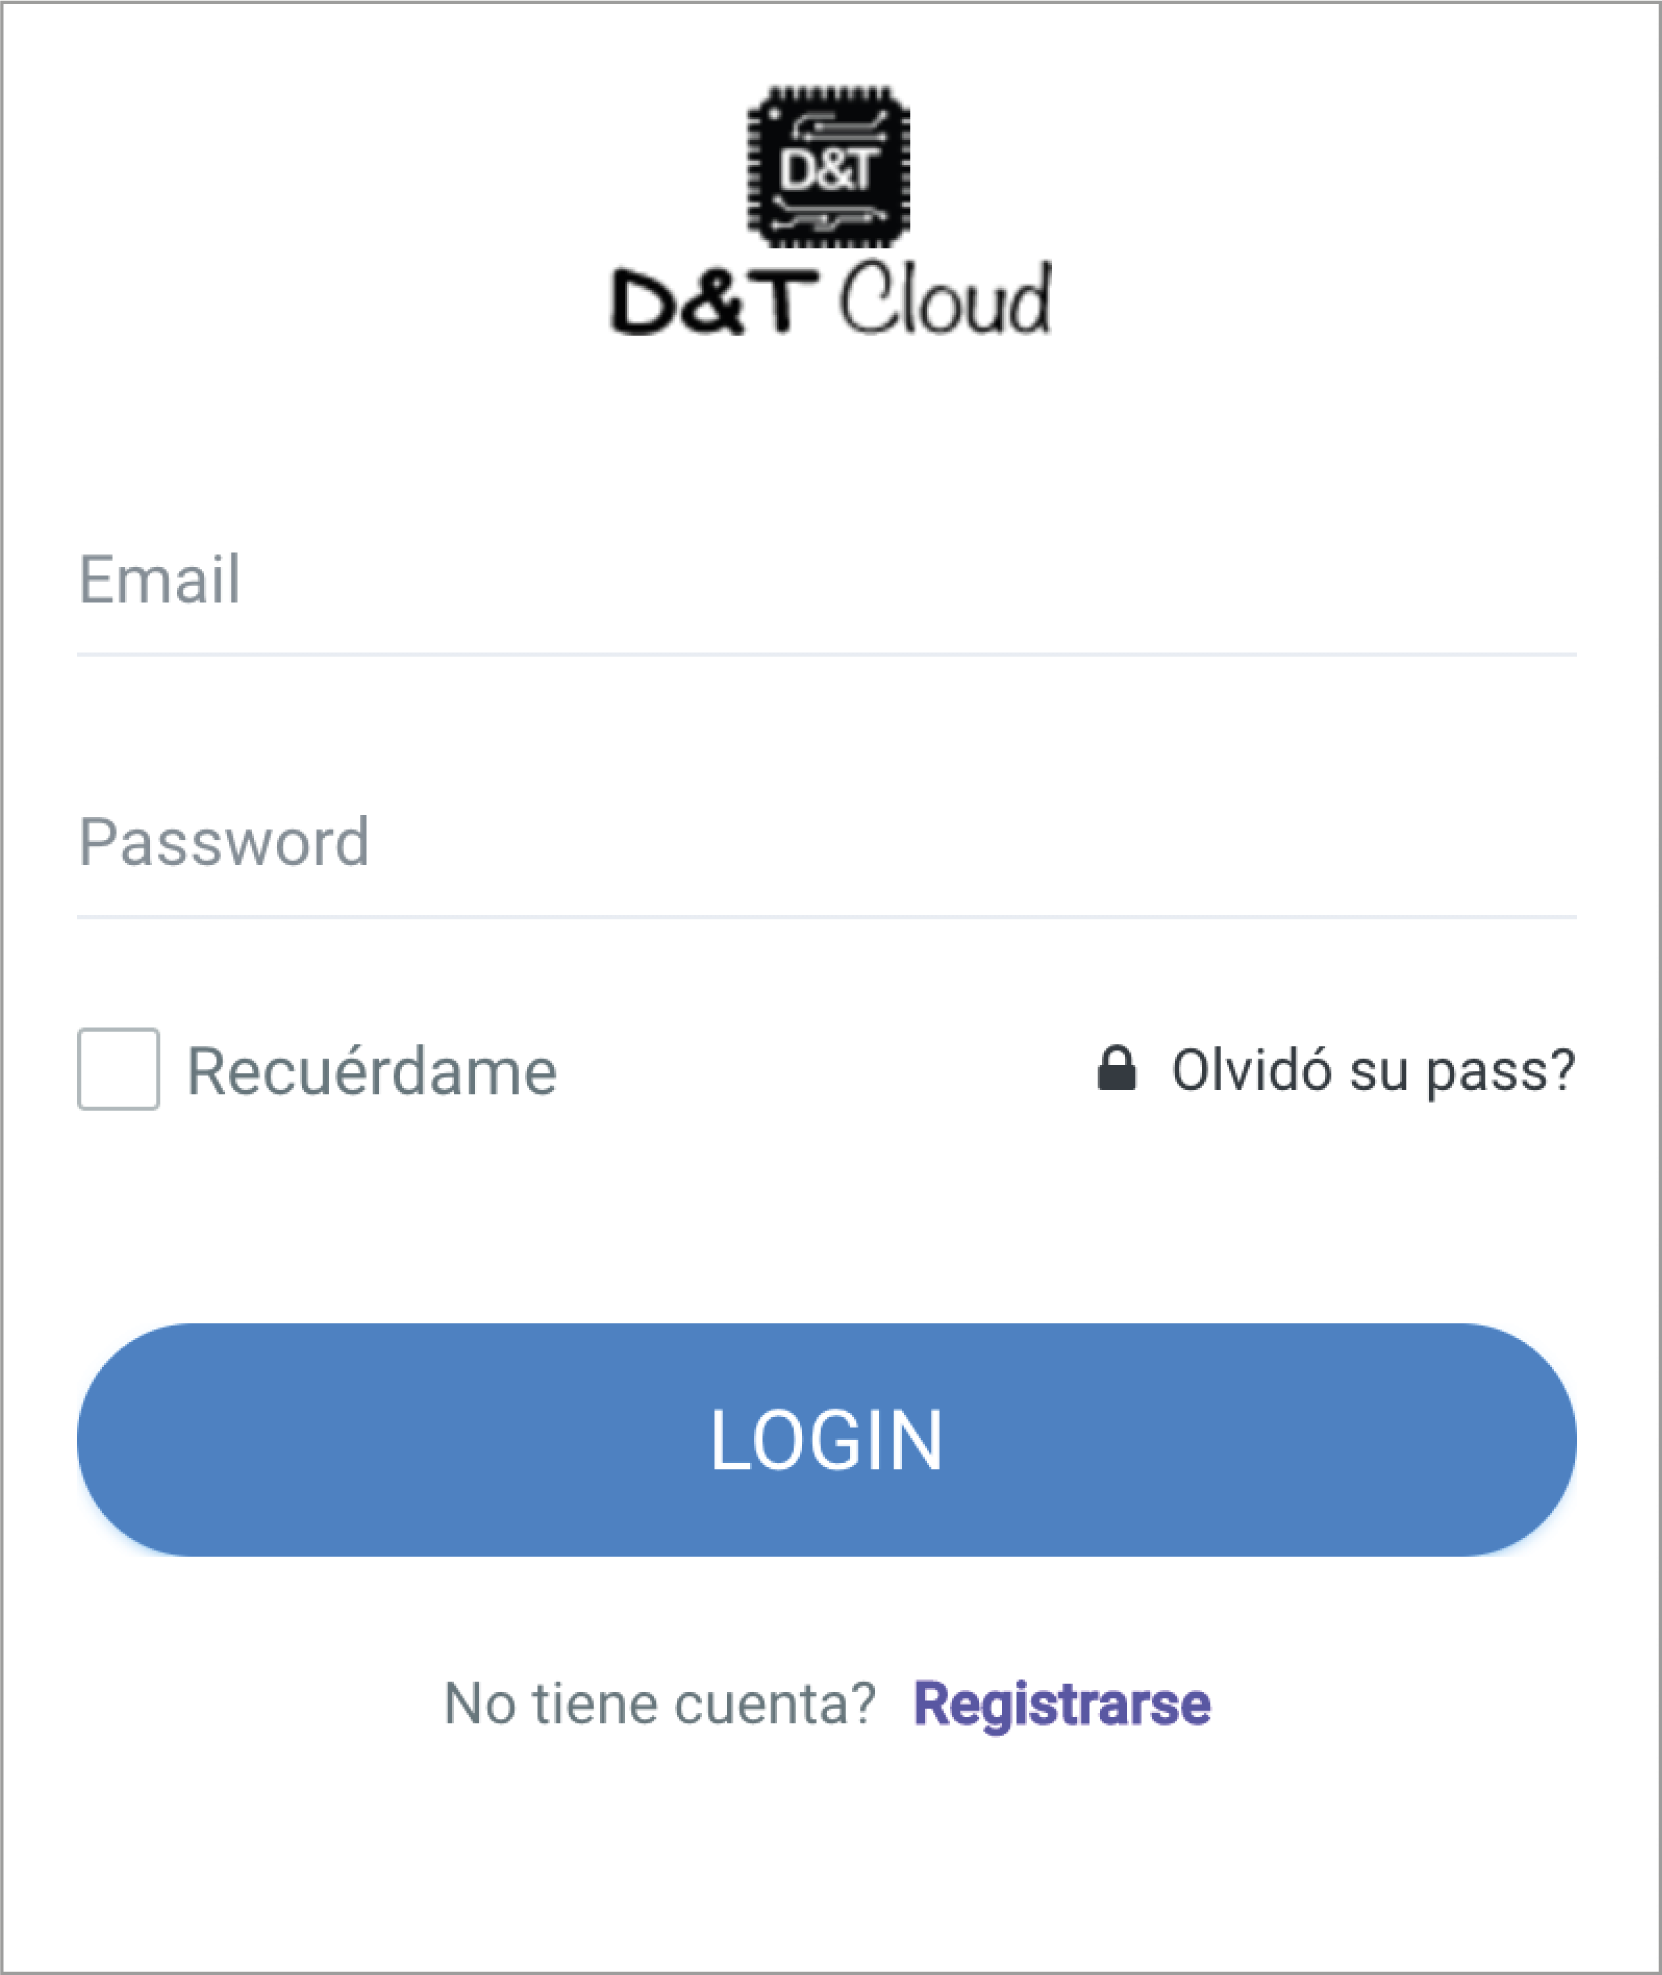
\includegraphics[scale=.75]{./Figures/pantalla-login.png}
	\caption[Pantalla de login y registro]{Ilustración de pantallas de login y registro de usuarios en plataforma web.}
	\label{fig:pantalla-login}
\end{figure}

Para la implementación en Angular, dentro de la carpeta /src se creo un componente para la pantalla de login y un componente para la pantalla de registro. En la figura \ref{fig:estructura-login} puede observarse la estructura y archivos creados para el desarrollo de las pantallas antes mencionadas. 

\begin{figure}[htpb]
	\centering
	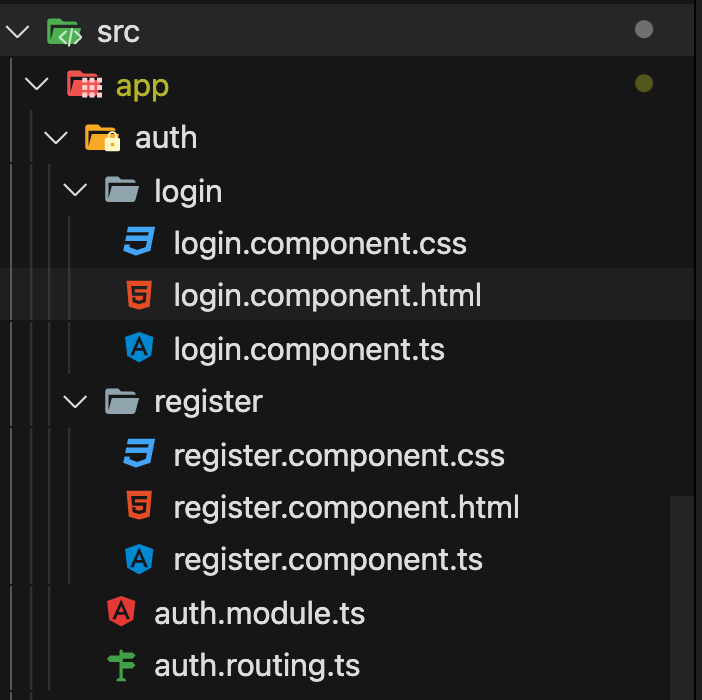
\includegraphics[scale=.50]{./Figures/estructura-login-vs.png}
	\caption[Estructura de componentes de login y registro]{Ilustración de estructura creada en el desarrollo de la pantalla de login y registro.}
	\label{fig:estructura-login}
\end{figure}

Los comandos de angular utilizados para crear estos componentes se pueden observar en el código \ref{cod:crear-componentes}.

\begin{lstlisting}[label=cod:crear-componentes,caption=Comandos de Angular para crear componentes de login y registro.] 

// Comando para crear el componente login en la carpeta auth
ng create component auth/login
// Comando para crear el componente register en la carpeta auth
ng create component auth/register

\end{lstlisting} 

Para la programación del componente login, se utilizó una plantilla HTML para formar la imagen deseada y utilizar dos campos de texto para introducir el usuario y contraseña.  En el código \ref{cod:html-login}. se puede observar la implementación de los aspectos principales de la pantalla teniendo en cuenta que además se utilizaron clases CSS para asignarle el estilo deseado. 

\begin{lstlisting}[label=cod:html-login,caption=Desarrollo de código HTML para la pantalla de login teniendo en cuenta estilos de diseño CSS.] 

<div class="card-body">

            <form (submit)="login()" 
                 class="form-horizontal form-material" 
                 id="loginform"
                 autocomplete="off"
                 [formGroup]= "loginForm">
               
                <div class="form-group m-t-40">
                    <div class="col-xs-12">
                        <input class="form-control" 
                            type="email" 
                            placeholder="Email"
                            formControlName='email'
                            >
                    </div>
                </div>
                <div class="form-group">
                    <div class="col-xs-12">
                        <input class="form-control" 
                                type="password"
                                placeholder="Password"
                                formControlName='password'>
                    </div>
                </div>
                
                <div class="form-group text-center m-t-20">
                    <div class="col-xs-12">
                        <button class="btn btn-info btn-lg btn-block text-uppercase btn-rounded" 
                            type="submit"
                            [class.spinner]="isLoading" [disabled]="isLoading">Log In</button>
                    </div>
                </div>
                      
            </form>
        </div>


\end{lstlisting} 

Otro aspecto importante en el desarrollo de la pantalla es la programación del comportamiento de cada campo en el que el usuario interactúa con la página. El código muestra las funciones principales que se programaron en el archivo \textit{Typescript}.

\begin{lstlisting}[label=cod:ts-login,caption=Fragmentos de código mas relevantes utilizado en el archivo \textit{Typescript} del componente login.] 

// Definicion de clase LoginComponent
export class LoginComponent {

  public formSubmitted = false;
  public isLoading = false;

  public loginForm = this.fb.group({  
    email:[localStorage.getItem('email') || '', [Validators.required, Validators.email]],
    password: ['', Validators.required],
    remember: [false]
  });

// Constructor de la clase donde se incluyen servicios para utilizar
  constructor(private router:Router,
              private fb: FormBuilder,
              private usuarioService: UsuarioService,
              private sweetAlert:SweetAlertService
              ) { }
              
// Metodo login(), cuando el usuario presiona el boton
  login(){
    this.formSubmitted = true;
    this.isLoading = true;
    if(this.loginForm.invalid){
      this.isLoading = false;
      return;
    }
// Validacion del formulario 
    if (this.loginForm.get('remember').value){
      localStorage.setItem('email',this.loginForm.get('email').value)
    }else{
      localStorage.removeItem('email');
    }
// Utilizacion de servicio inyectado en el constructor.
    this.usuarioService.loginUsuario(this.loginForm.value)
      .subscribe(resp => {
        console.log('login correcto', resp);
        this.isLoading = false;
// Si el login es correcto, navega a la pagina principal. 
        this.router.navigateByUrl('/');
      },
      (err) => {
        console.log(err);
        this.isLoading = false;
        this.sweetAlert.showAlert(
          'Error',
          err.error.msg,
          'error',
          'Ok'
        );
      });
    
  }

}
\end{lstlisting} 

Otro aspecto importante del frontend es la programación de un servicio que permita conectarse con el backend y realizar peticiones HTTP. Para el caso de la pantalla de login,  se requiere acceder a la base de datos para verificar si el email y password utilizado por el usuario son correctos y así poder acceder a la pagina principal. 

El código \ref{cod:service-login} muestra la implementación de un servicio que es utilizado por el componente de login de usuario. En él puede observarse un método llamado loginUsuario el cual realiza una petición POST al backend.  Luego espera una respuesta por parte de la petición para verificar si la misma es correcta.  Por otro lado se programó un método crearUsuario el cual crea un nuevo usuario en la base de datos, utilizando las funciones CRUD programadas en el backend. 

\begin{lstlisting}[label=cod:service-login,caption=Fragmentos de código mas relevantes utilizados en el servicio de usuario.] 

export class UsuarioService {

  public usuario: UserModel;

  constructor(private http: HttpClient,
              private router: Router) { }

  crearUsuario( formData: RegisterForm){
    return this.http.post(`${base_url}/usuario`, formData );
  }
  
  loginUsuario( formData: LoginForm){
    return this.http.post(`${base_url}/login`, formData )
      .pipe(
        tap( (resp:any) =>{
          localStorage.setItem('token', resp.token);
          localStorage.setItem('menu', JSON.stringify(resp.menu));
          //sessionStorage.setItem('user_id', resp.id._id);
        })
      );
  }
}

\end{lstlisting} 

En general, toda la implementación del frontend está basada en estas tres implementaciones de código.  La metodología adoptada fue crear componentes por cada una de las funcionalidades donde el usuario interactúa con la plataforma y a su vez la utilidad de los servicios para interactuar entre el backend y el frontend teniendo en cuenta las consultas a la base de datos. 

Por otro lado para observar los datos en tiempo real provenientes de los dispositivos conectados al broker MQTT, es necesario que el frontend pueda acceder y suscribirse a los tópicos a los que estos dispositivos están publicando. 

Para ello se utiliza la librería ngx-mqtt\citep{WEBSITE:41} que permite crear un cliente MQTT a través del uso de websockets\citep{WEBSITE:42}. El código \ref{cod:mqtt-angular} muestra la forma de realizar la conexión con el broker MQTT utilizando el puerto seguro 884 descrito en la sección \ref{mqtt-sec}. Luego en cada componente que se utiliza la conexión se implementan los métodos de suscripción y publicación. 

\begin{lstlisting}[label=cod:mqtt-angular,caption=Implementación de cliente MQTT en Angular utilizando la librería ngx-mqtt.] 
// Definicion de parametros de conexion

mqtt_b: {
    connectOnCreate: true,
    protocol: "wss",
    host: "host.al.broker",
    port: 884,
    path: "",
    username: "user",
    password: "pass",
    keepalive: 60,
    reconnectPeriod: 1000,
    test: false,
  },
  
  // Configuracion del servicio de la libreria MQTT
  const MQTT_SERVICE_OPTIONS: IMqttServiceOptions = {
  clientId:'mqtt_dyt',
  connectOnCreate: environment.mqtt_b.connectOnCreate,
  protocol: (environment.mqtt_b.protocol === "wss") ? "wss" : "ws",
  hostname: environment.mqtt_b.host,
  port: environment.mqtt_b.port,
  path: environment.mqtt_b.path,
  username: environment.mqtt_b.username,
  password: environment.mqtt_b.password,
  keepalive: environment.mqtt_b.keepalive,
  reconnectPeriod: environment.mqtt_b.reconnectPeriod,
};

\end{lstlisting} 

Una vez que el usuario realiza el login de forma exitosa, puede acceder a las diferentes pantallas de la plataforma. En la figura \ref{fig:bloque-pantallas} se puede observar un diagrama de todas las rutas implementadas en el trabajo a las que un usuario puede acceder. 

\begin{figure}[htpb]
	\centering
	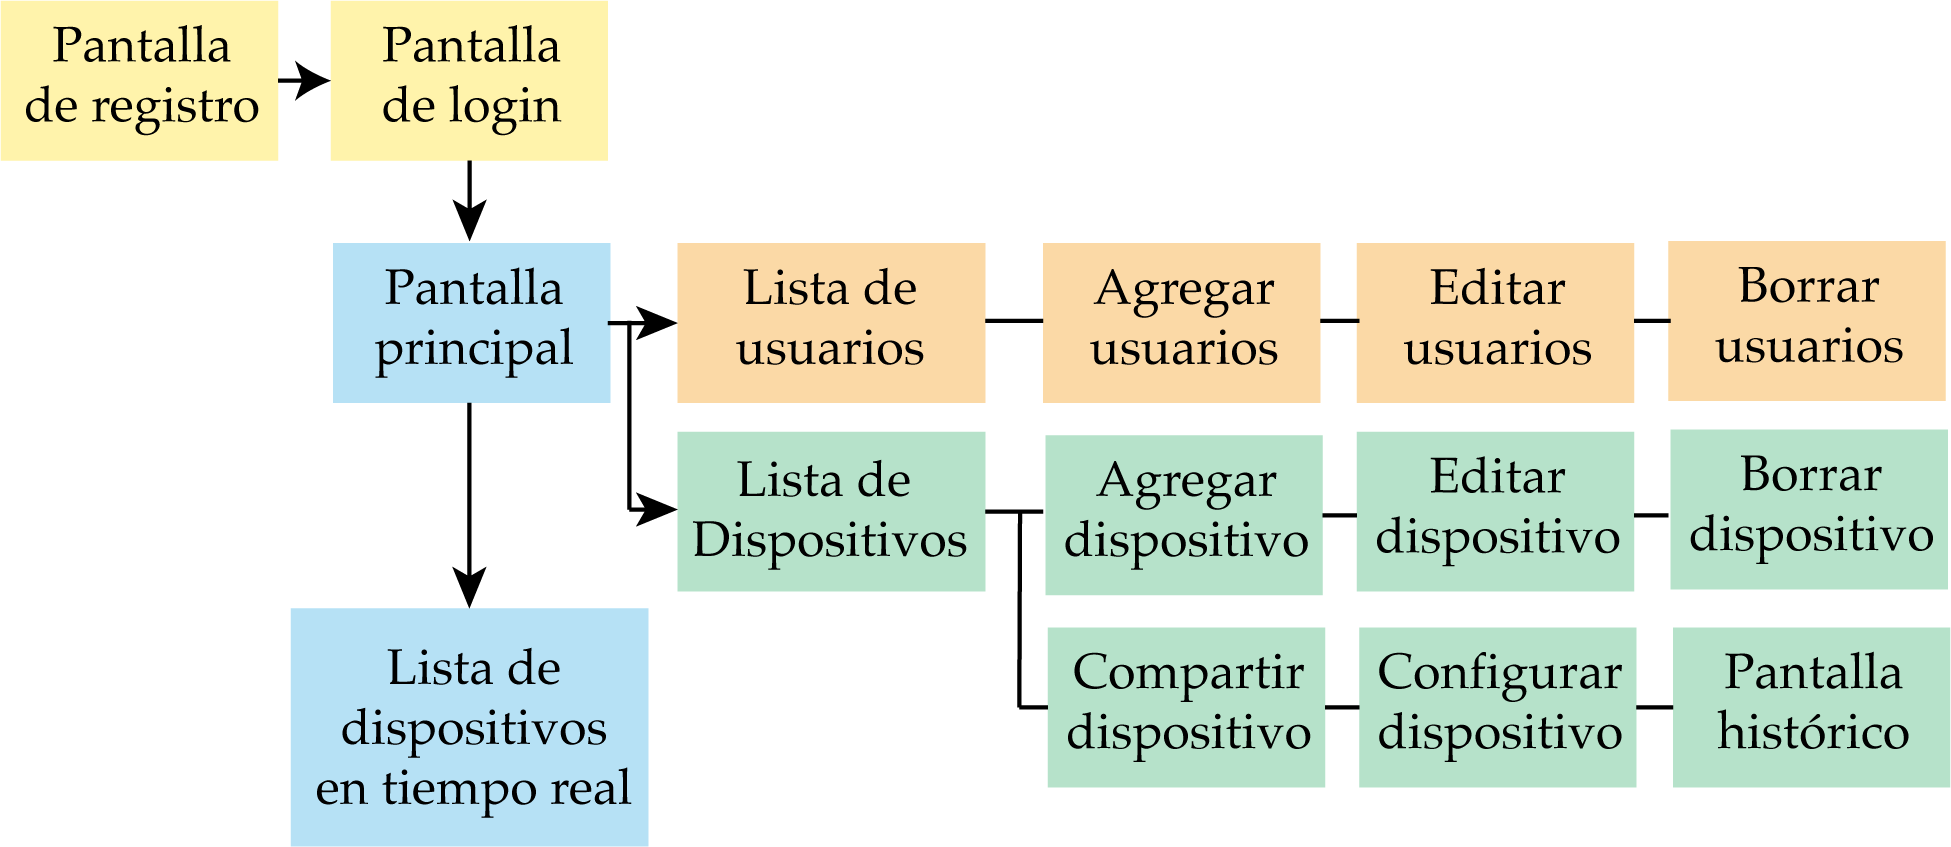
\includegraphics[scale=.75]{./Figures/bloques-pantallas.png}
	\caption[Rutas del sistema]{Ilustración de bloques con rutas implementadas en el sistema.}
	\label{fig:bloque-pantallas}
\end{figure}

Cuando un usuario se registra a la plataforma, por defecto es un usuario administrador. Este rol le permite acceder y crear nuevos usuarios donde puede asignar roles de operador. 

El rol operador, solo permite a los usuarios visualizar información referida a los dispositivos conectados, invalidando la posibilidad de editar, borrar o agregar dispositivos y usuarios.

En la pantalla principal o también llamada \textit{dashboard}, se muestran dispositivos que se encuentran agregados al sistema por parte de un usuario administrador. Estos, son leídos desde la base de datos cuando el usuario ingresa a la plataforma y se adaptan a un modelo de sensor cargado en el sistema. En la figura \ref{fig:dashboard} se muestran dos dispositivos que hacen referencia a sensores de temperatura fabricados por la empresa D\&T que utilizan el modulo conversor Modbus a MQTT..  

 \begin{figure}[htpb]
	\centering
	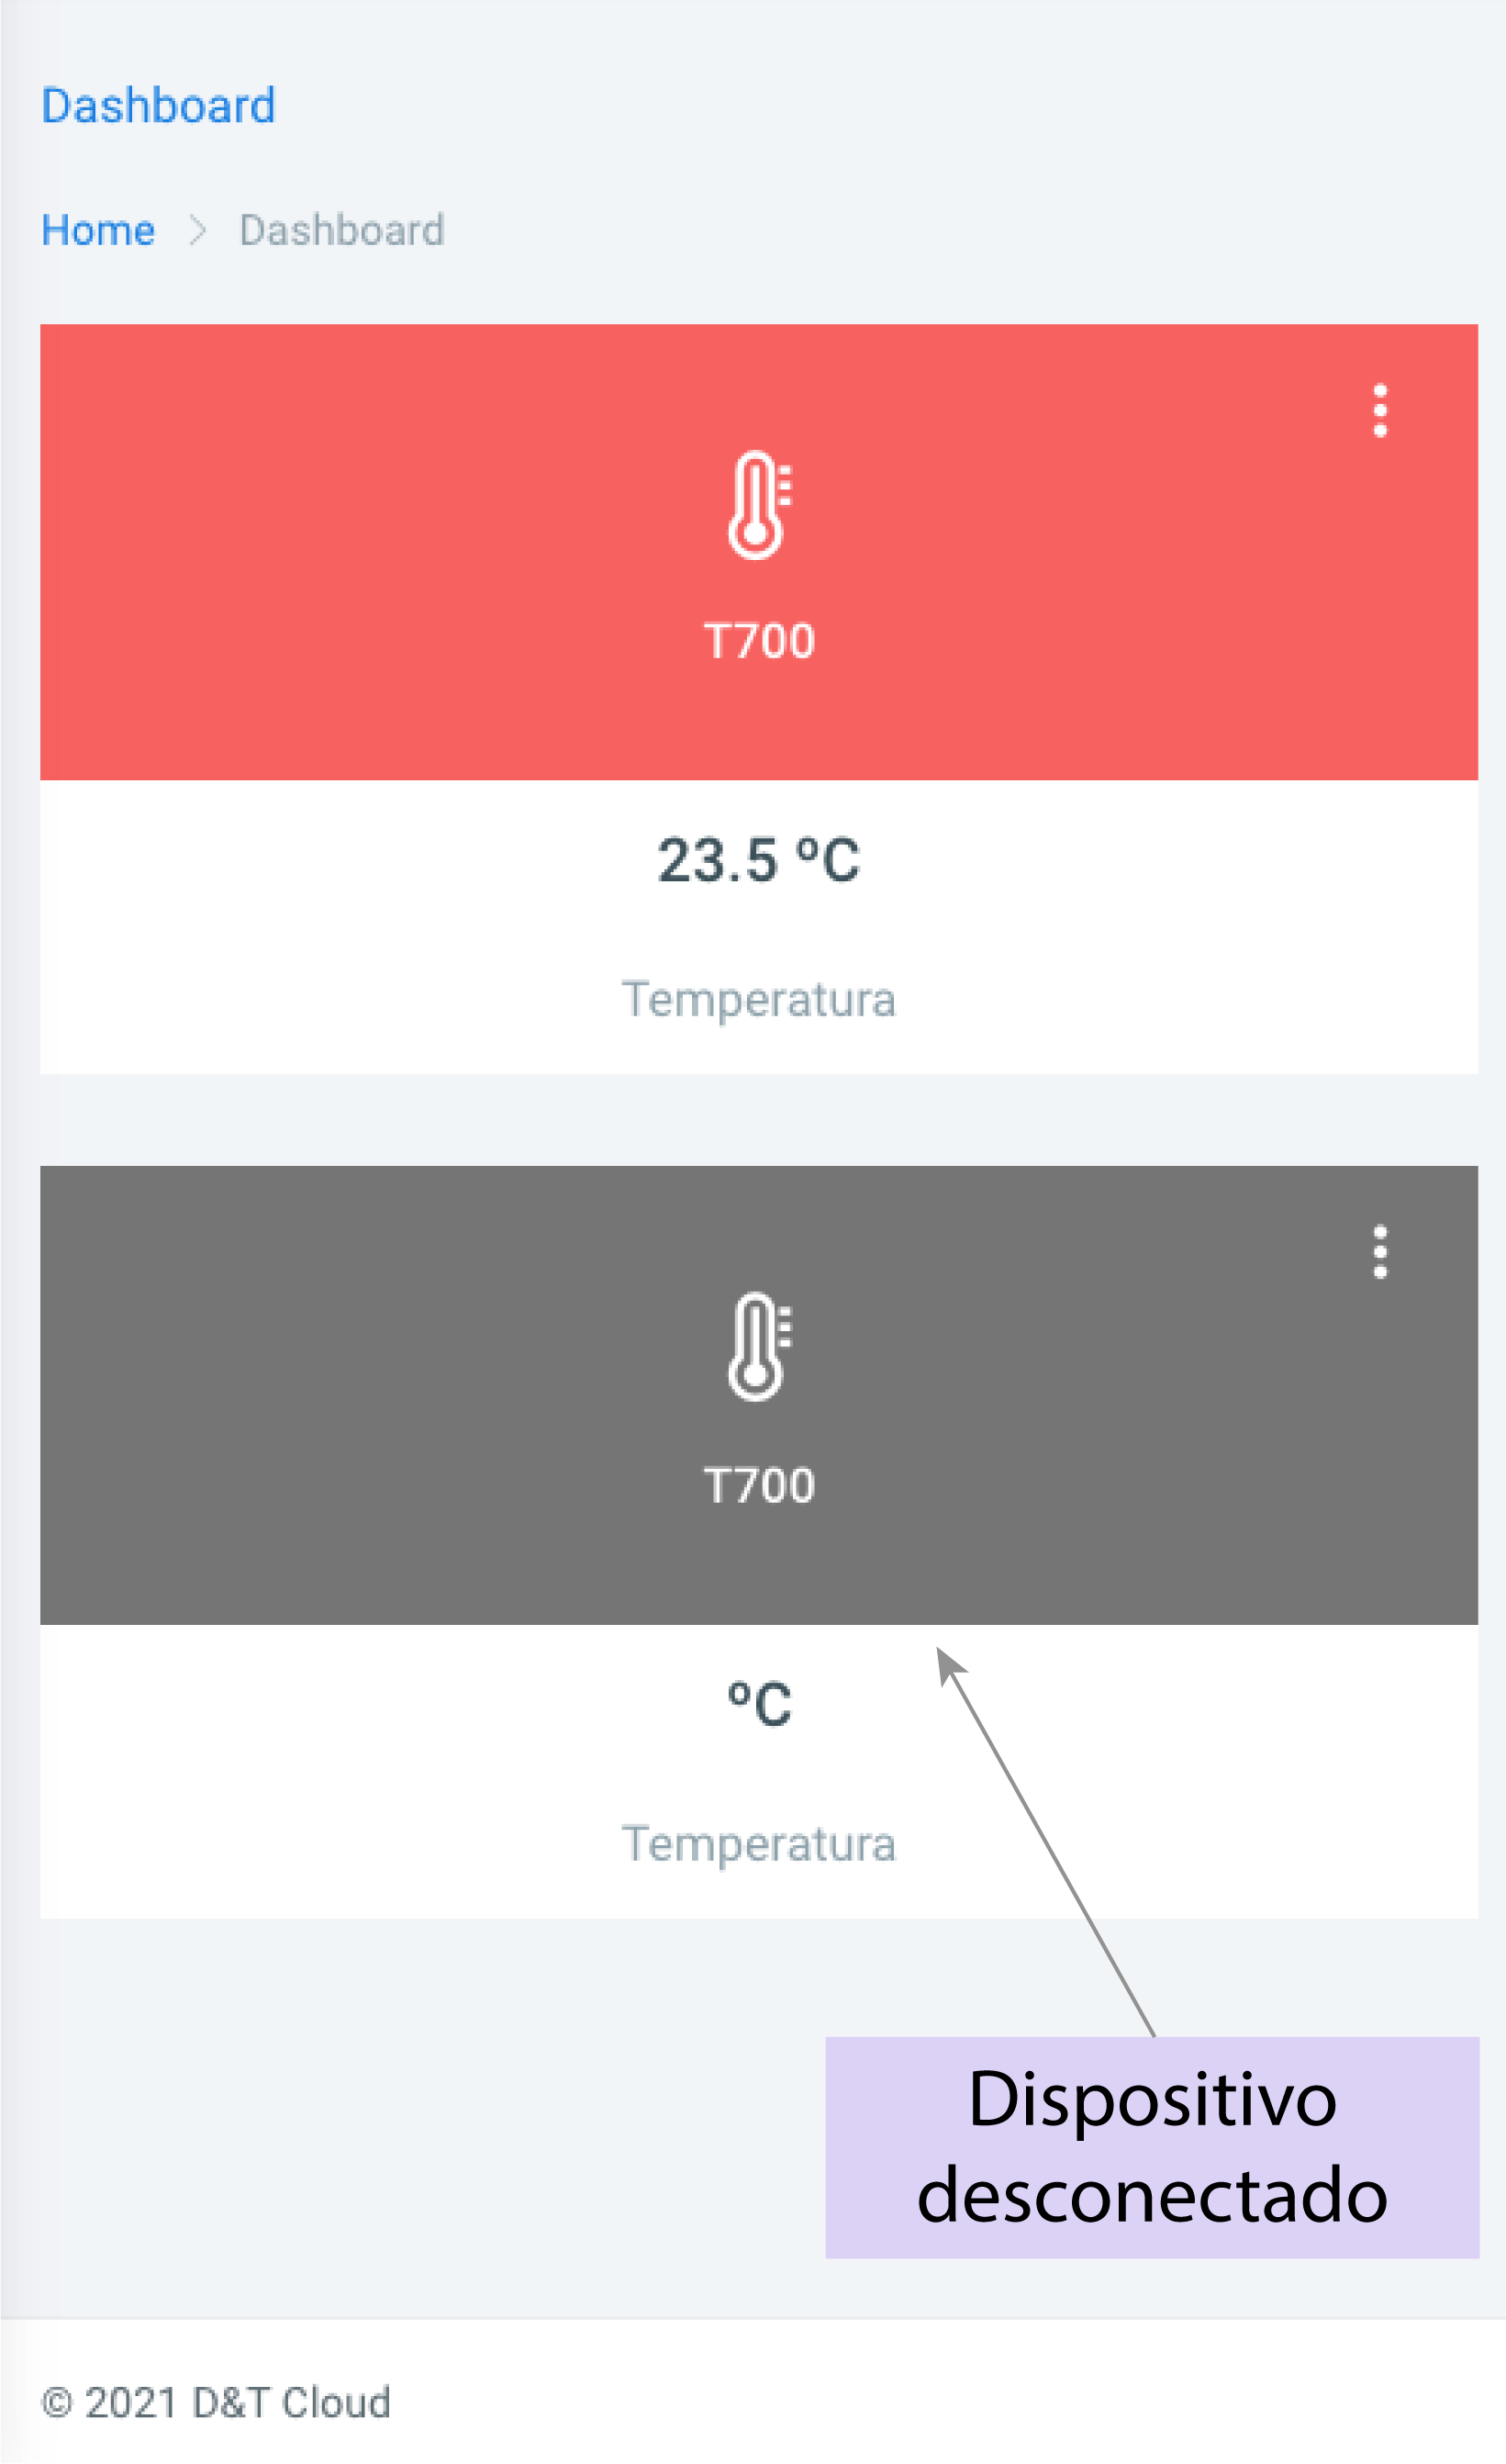
\includegraphics[scale=.25]{./Figures/dashboard.png}
	\caption[Pantalla principal - \textit{dashboard}]{Ilustración de lista de sensores de temperatura T700 conectados a conversores Modbus a MQTT. }
	\label{fig:dashboard}
\end{figure}


Cada bloque de sensor, corresponde a un componente de Angular, el cual tiene un servicio asociado para el manejo de datos en tiempo real y además la posibilidad de acceder a sus datos históricos. En la figura \ref{fig:sensor-temp} se observa en detalle las opciones de acceso implementadas en el componente.

 \begin{figure}[htpb]
	\centering
	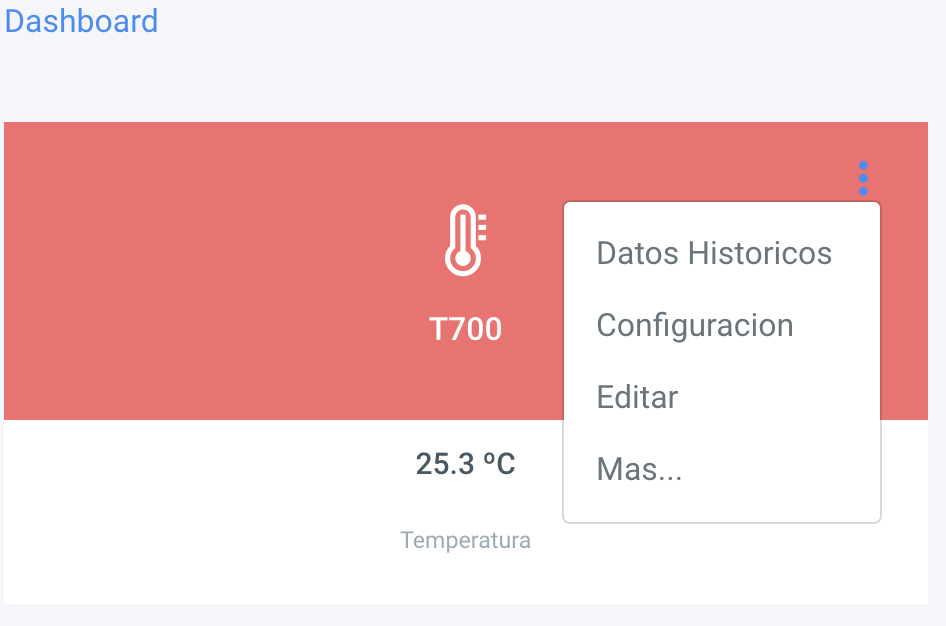
\includegraphics[scale=.40]{./Figures/sensor-temp.png}
	\caption[Sensor de temperatura T700]{Ilustración de componente utilizado para modelar el sensor T700 y sus opciones de acceso.}
	\label{fig:sensor-temp}
\end{figure}


Si el usuario requiere realizar cambios en el dispositivo y editar parámetros como se muestra en la figura \ref{fig:sensor-temp}, puede ingresar directamente desde el componente y sus accesos directos, o bien buscarlo en el listado de dispositivos y presionando en el botón de edición.

 \begin{figure}[htpb]
	\centering
	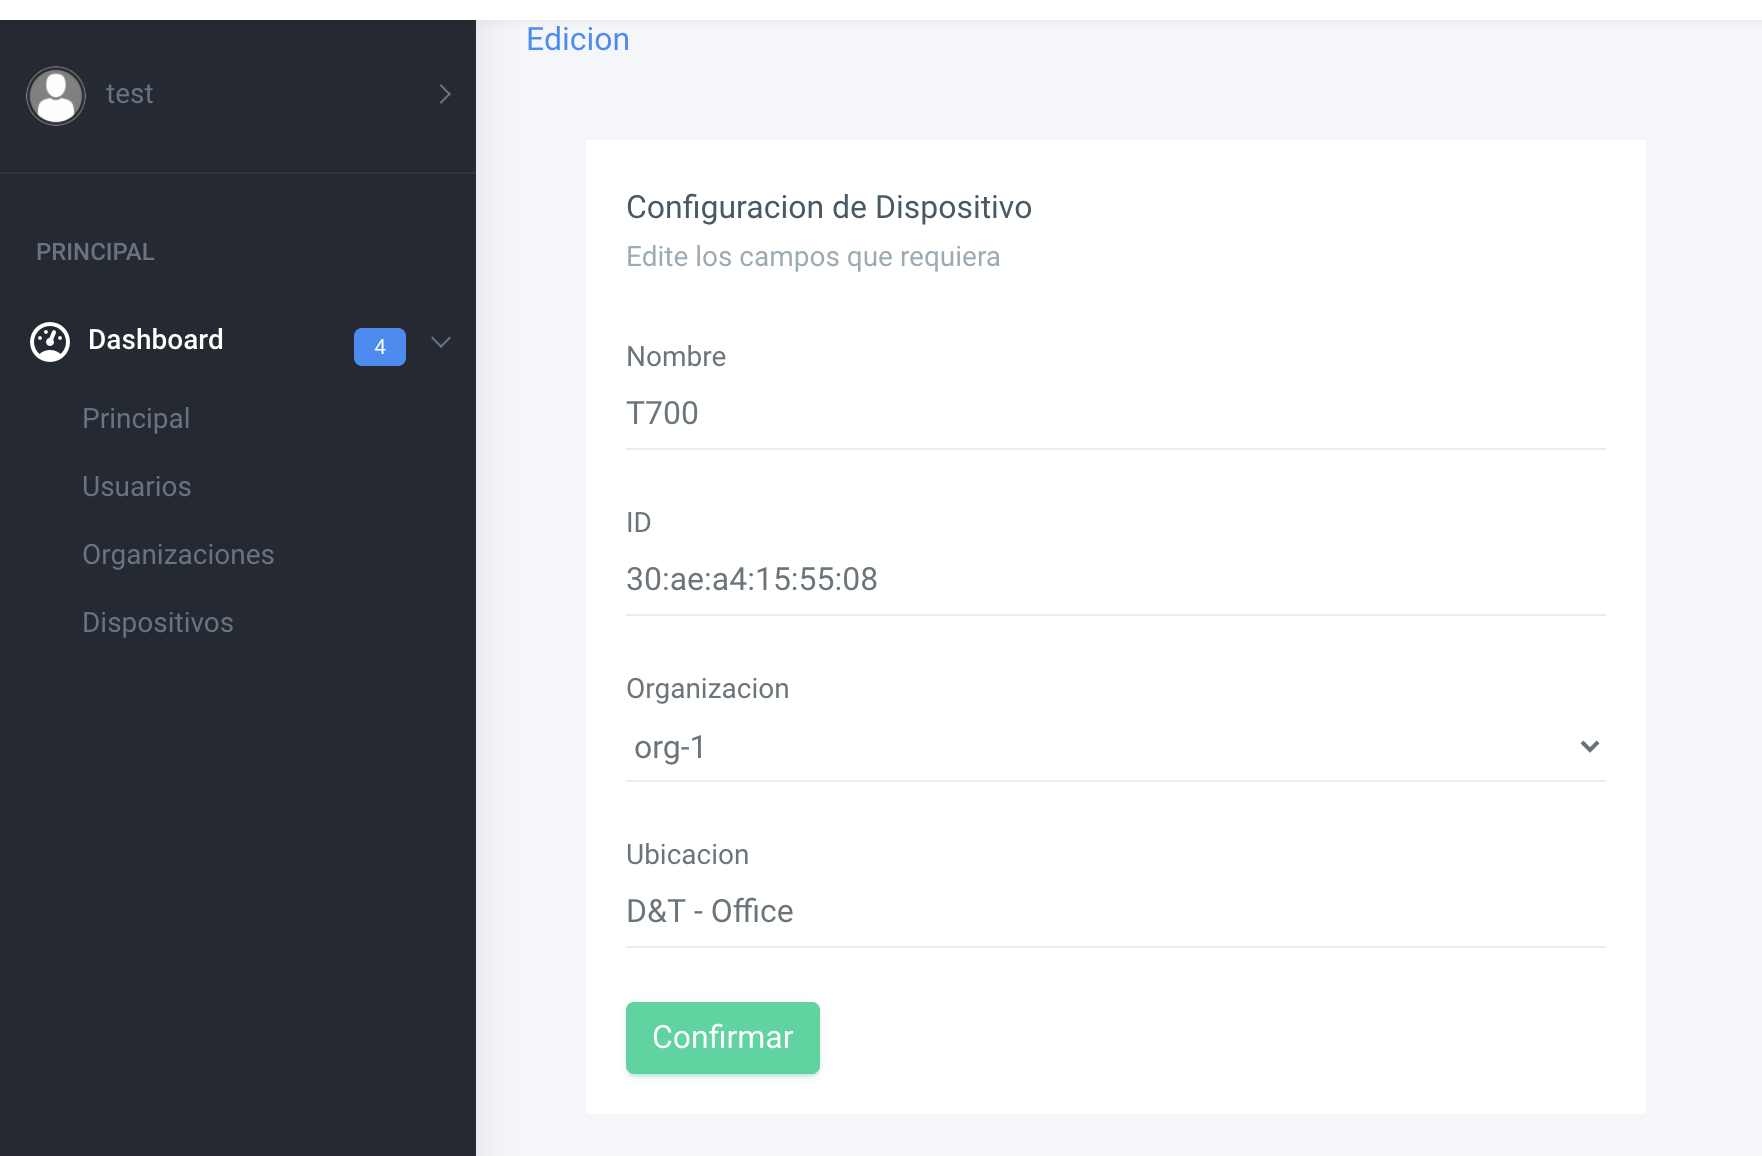
\includegraphics[scale=.30]{./Figures/edicion-dev.png}
	\caption[Pantalla de edición de dispositivos]{Ilustración de pantalla de edicion de dispositivos.}
	\label{fig:edicion-dev}
\end{figure}


Para la visualización de datos históricos de dispositivos se utilizo la librería para Angular echarts \citep{WEBSITE:43}. Esta amplia librería permite la utilización de gráficos para mostrar datos históricos de mediciones de los dispositivos que almacenan datos en MongoDB. En la figura \ref{fig:echart-grafica} puede observarse las características principales que ofrece el componente para realizar un gráfico y las opciones correspondientes.

\begin{figure}[htpb]
	\centering
	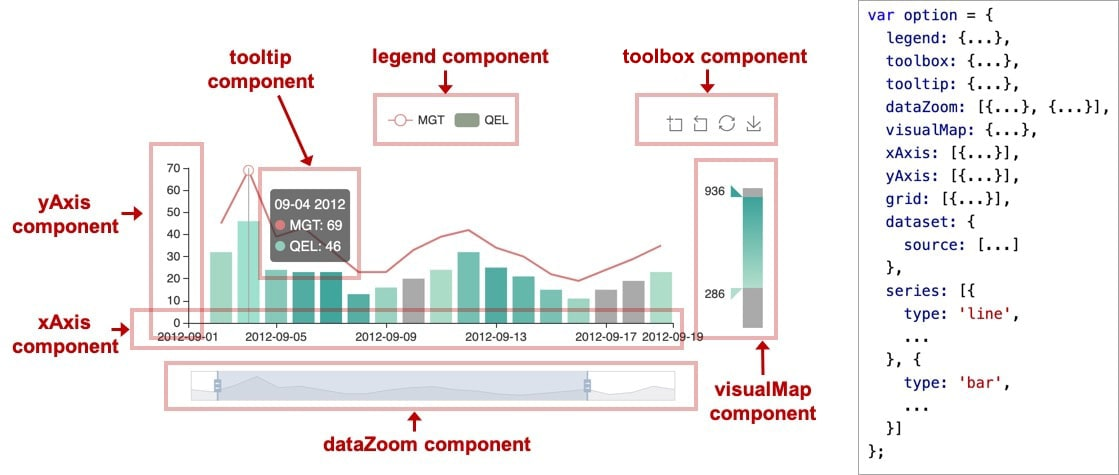
\includegraphics[scale=.30]{./Figures/echart-grafica.jpg}
	\caption[Componente gráfico de echarts]{Ilustración de componente gráfico utilizando la librería echart y opciones de configuración.}
	\label{fig:echart-grafica}
\end{figure}

En la plataforma se implementó un gráfico de lineas con la librería echarts teniendo en cuenta datos provenientes de la base de datos como se muestra en la figura \ref{fig:device-grafica}. Los datos corresponden a un sensor de temperatura que utiliza un dispositivo conversor de datos Modbus a MQTT.

\begin{figure}[htpb]
	\centering
	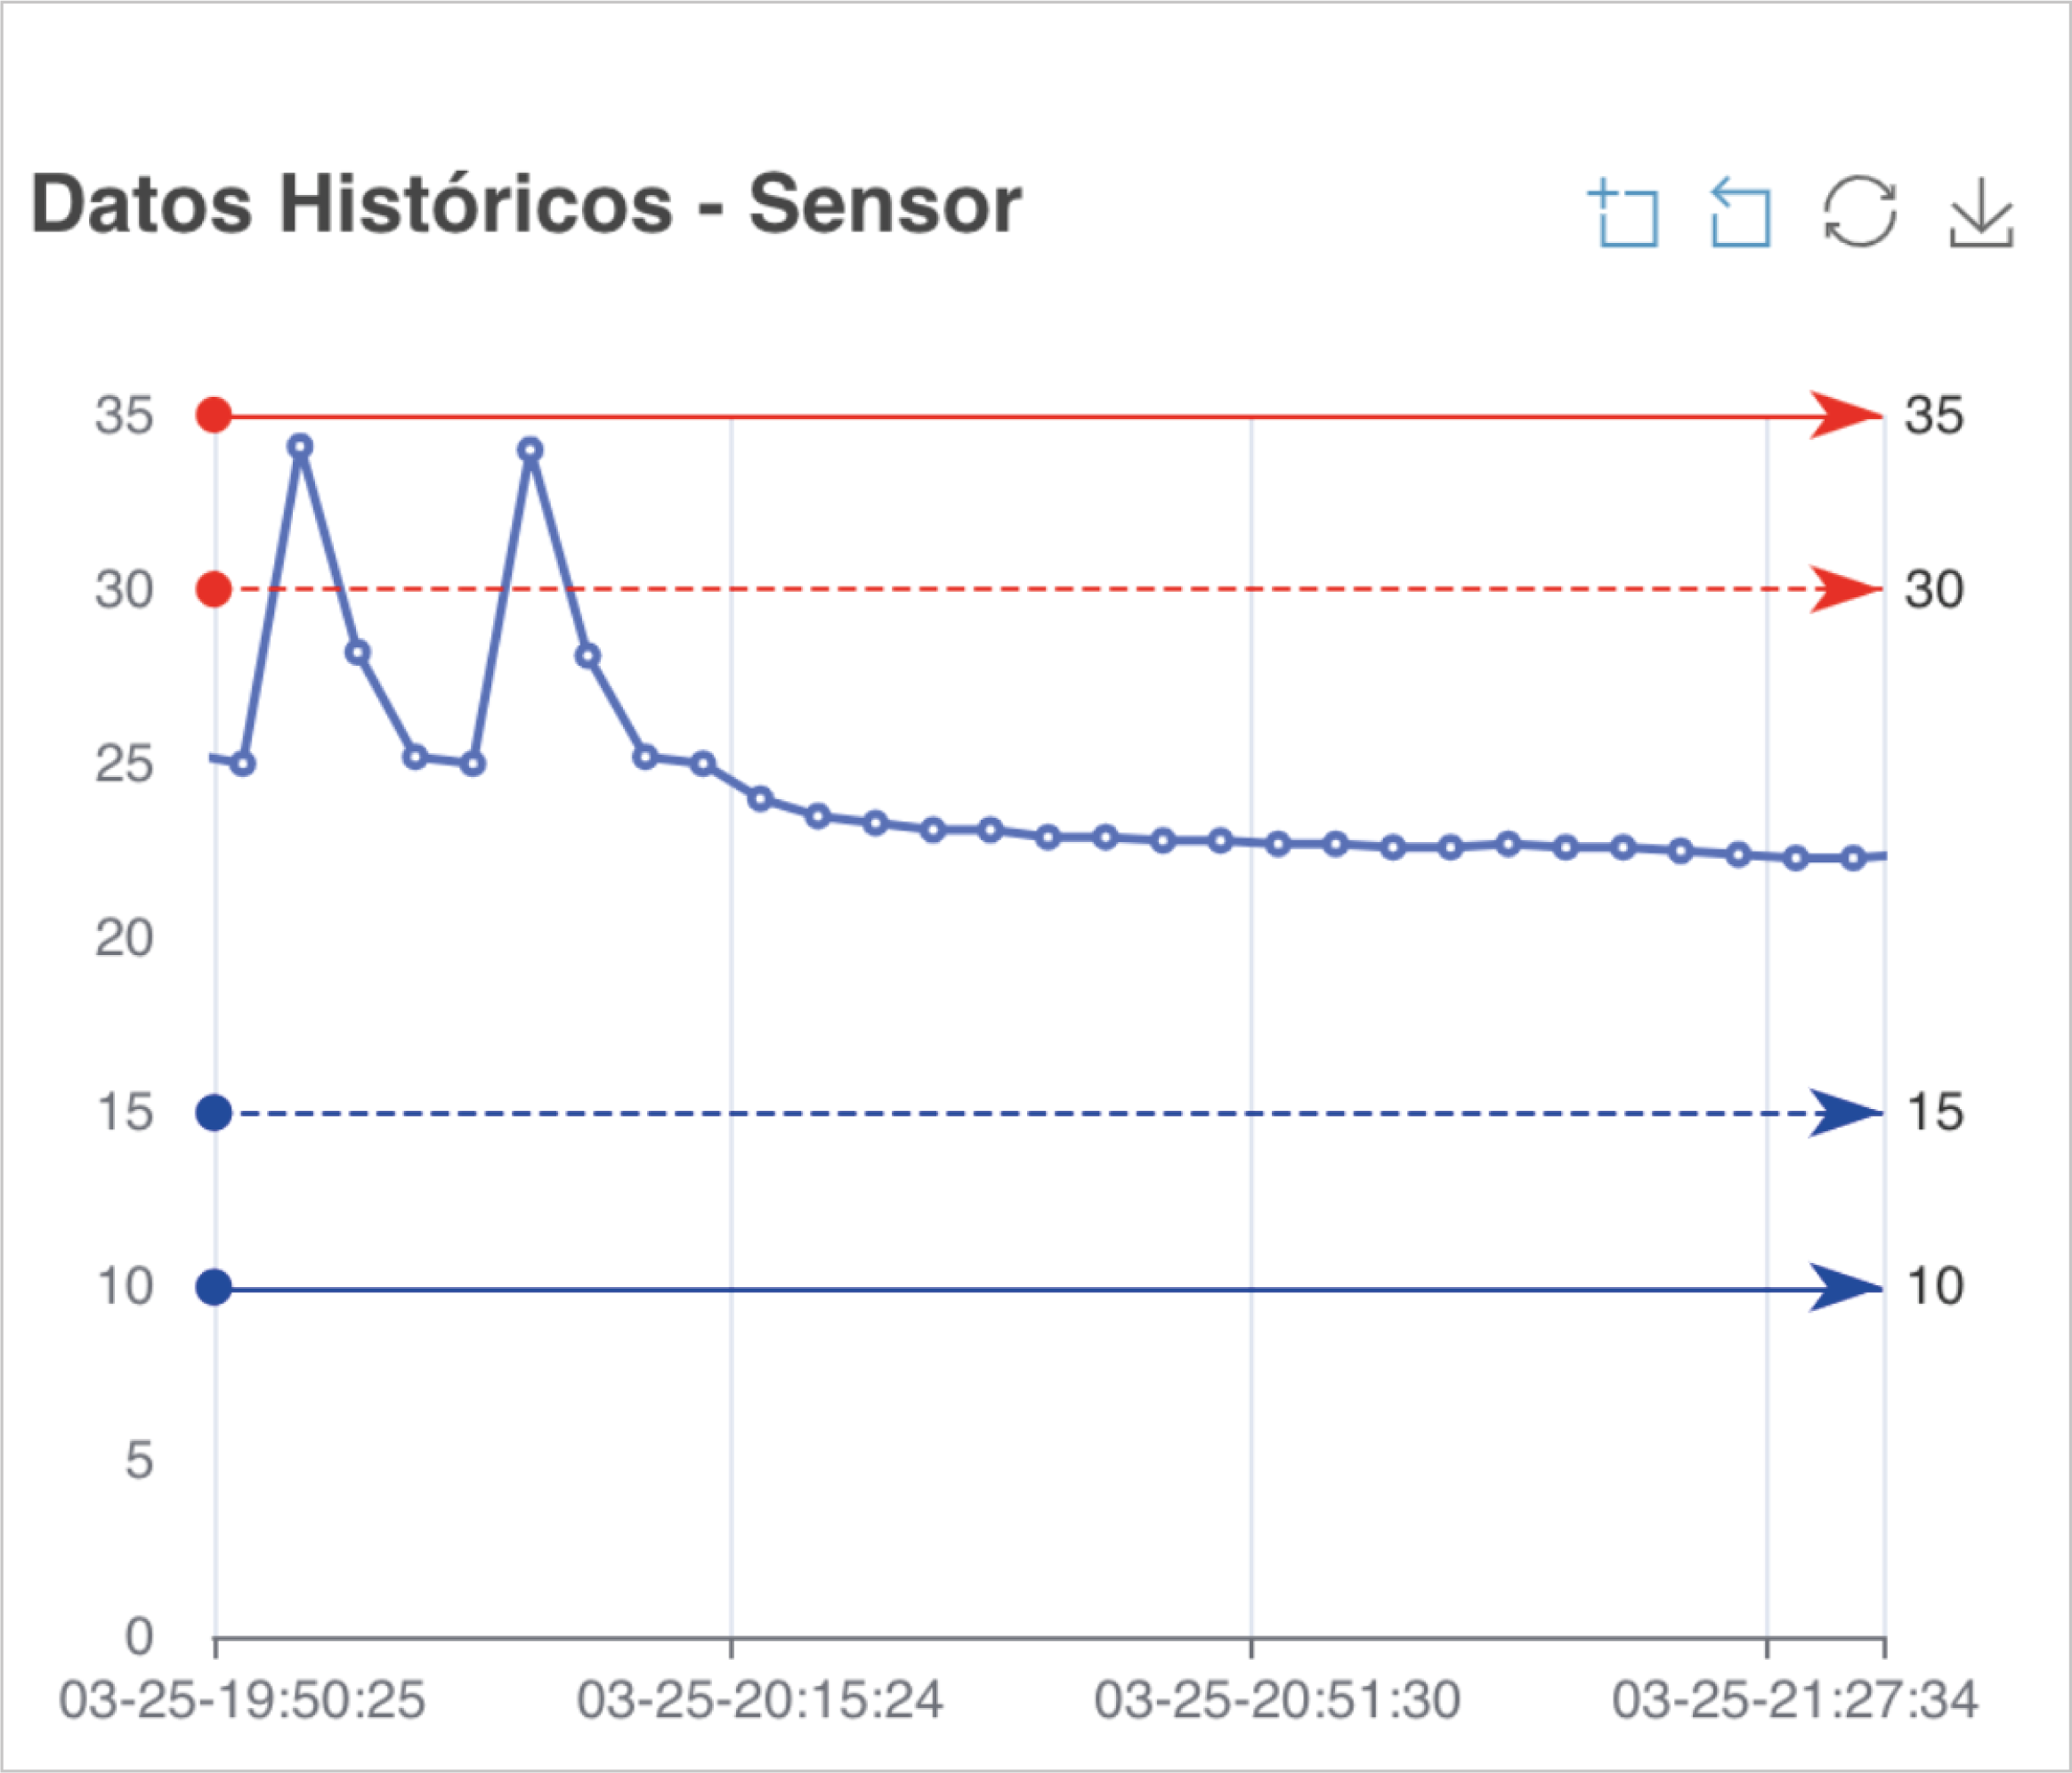
\includegraphics[scale=.30]{./Figures/device-grafica.png}
	\caption[Componente gráfico de echarts]{Ilustración de datos históricos de sensor de temperatura conectado a conversor de datos Modbus a MQTT.}
	\label{fig:device-grafica}
\end{figure}


El diseño web \textit{responsive} o adaptativo es una técnica de diseño web que busca la correcta visualización de una misma página en distintos dispositivos. Desde computadoras de escritorio a tablets y móviles.  Se trata de dimensionar y colocar los elementos de la web de forma que se adapten al ancho de cada dispositivo permitiendo una correcta visualización y una mejor experiencia de usuario.  Para el diseño de la plataforma se utilizaron componentes con estilos que se adaptan a diferentes tamaños de pantallas. 

En la figura \ref{fig:pantalla-pc}. se observa la visualización de la pantalla principal adaptada para pantallas que son utilizadas en PC de escritorio, se debe notar que el usuario puede visualizar el contenido completo, teniendo en cuenta la barra lateral desplegada con las opciones disponibles. 

\begin{figure}[htpb]
	\centering
	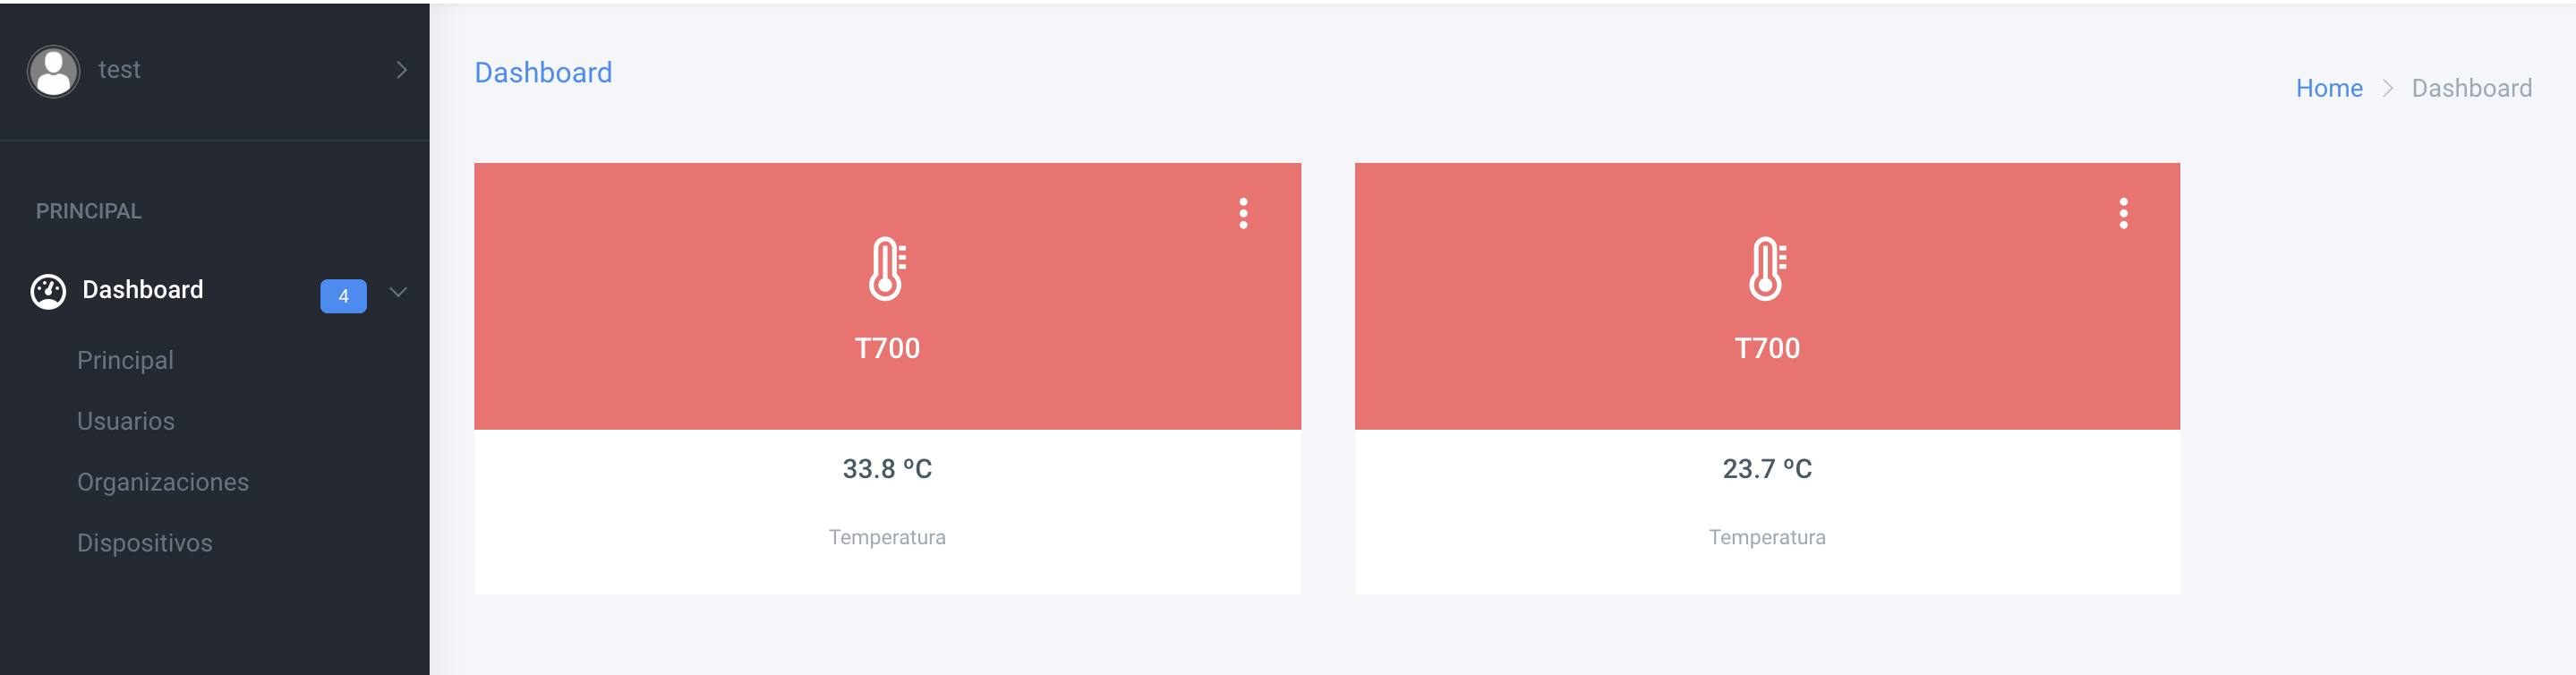
\includegraphics[scale=.20]{./Figures/pantalla-pc.png}
	\caption[Pantalla adaptada a pantallas para PC]{Ilustración de pantalla principal adaptada a pantallas de PC.}
	\label{fig:pantalla-pc}
\end{figure}

Por otro lado la figura \ref{fig:pantalla-tablet} se adapta a pantallas de tablets y que se encuentran de forma horizontal, donde se aprecia que la barra lateral se oculta y si el usuario necesita algún item deberá presionar el botón correspondiente para poder desplegarla. 

\begin{figure}[htpb]
	\centering
	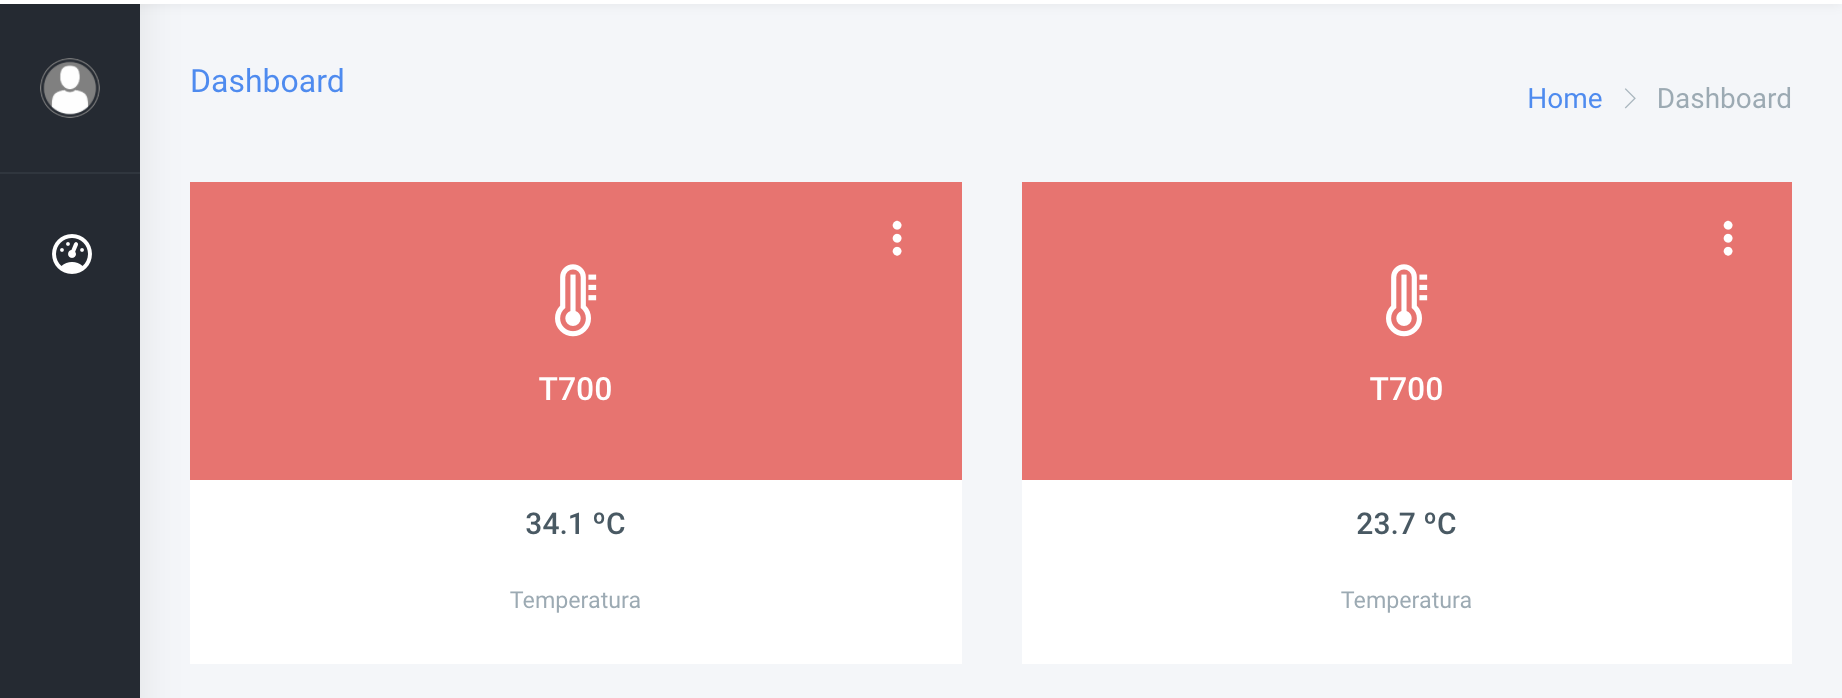
\includegraphics[scale=.25]{./Figures/pantalla-tablet.png}
	\caption[Pantalla adaptada a tablets]{Ilustración de pantalla principal adaptada a tablets.}
	\label{fig:pantalla-tablet}
\end{figure}

En ultima instancia, la figura \ref{fig:pantalla-celu} la pantalla para celulares adapta el listado de dispositivos a una sola columna y oculta la barra lateral para poder desplegarla a través de un botón.

\begin{figure}[htpb]
	\centering
	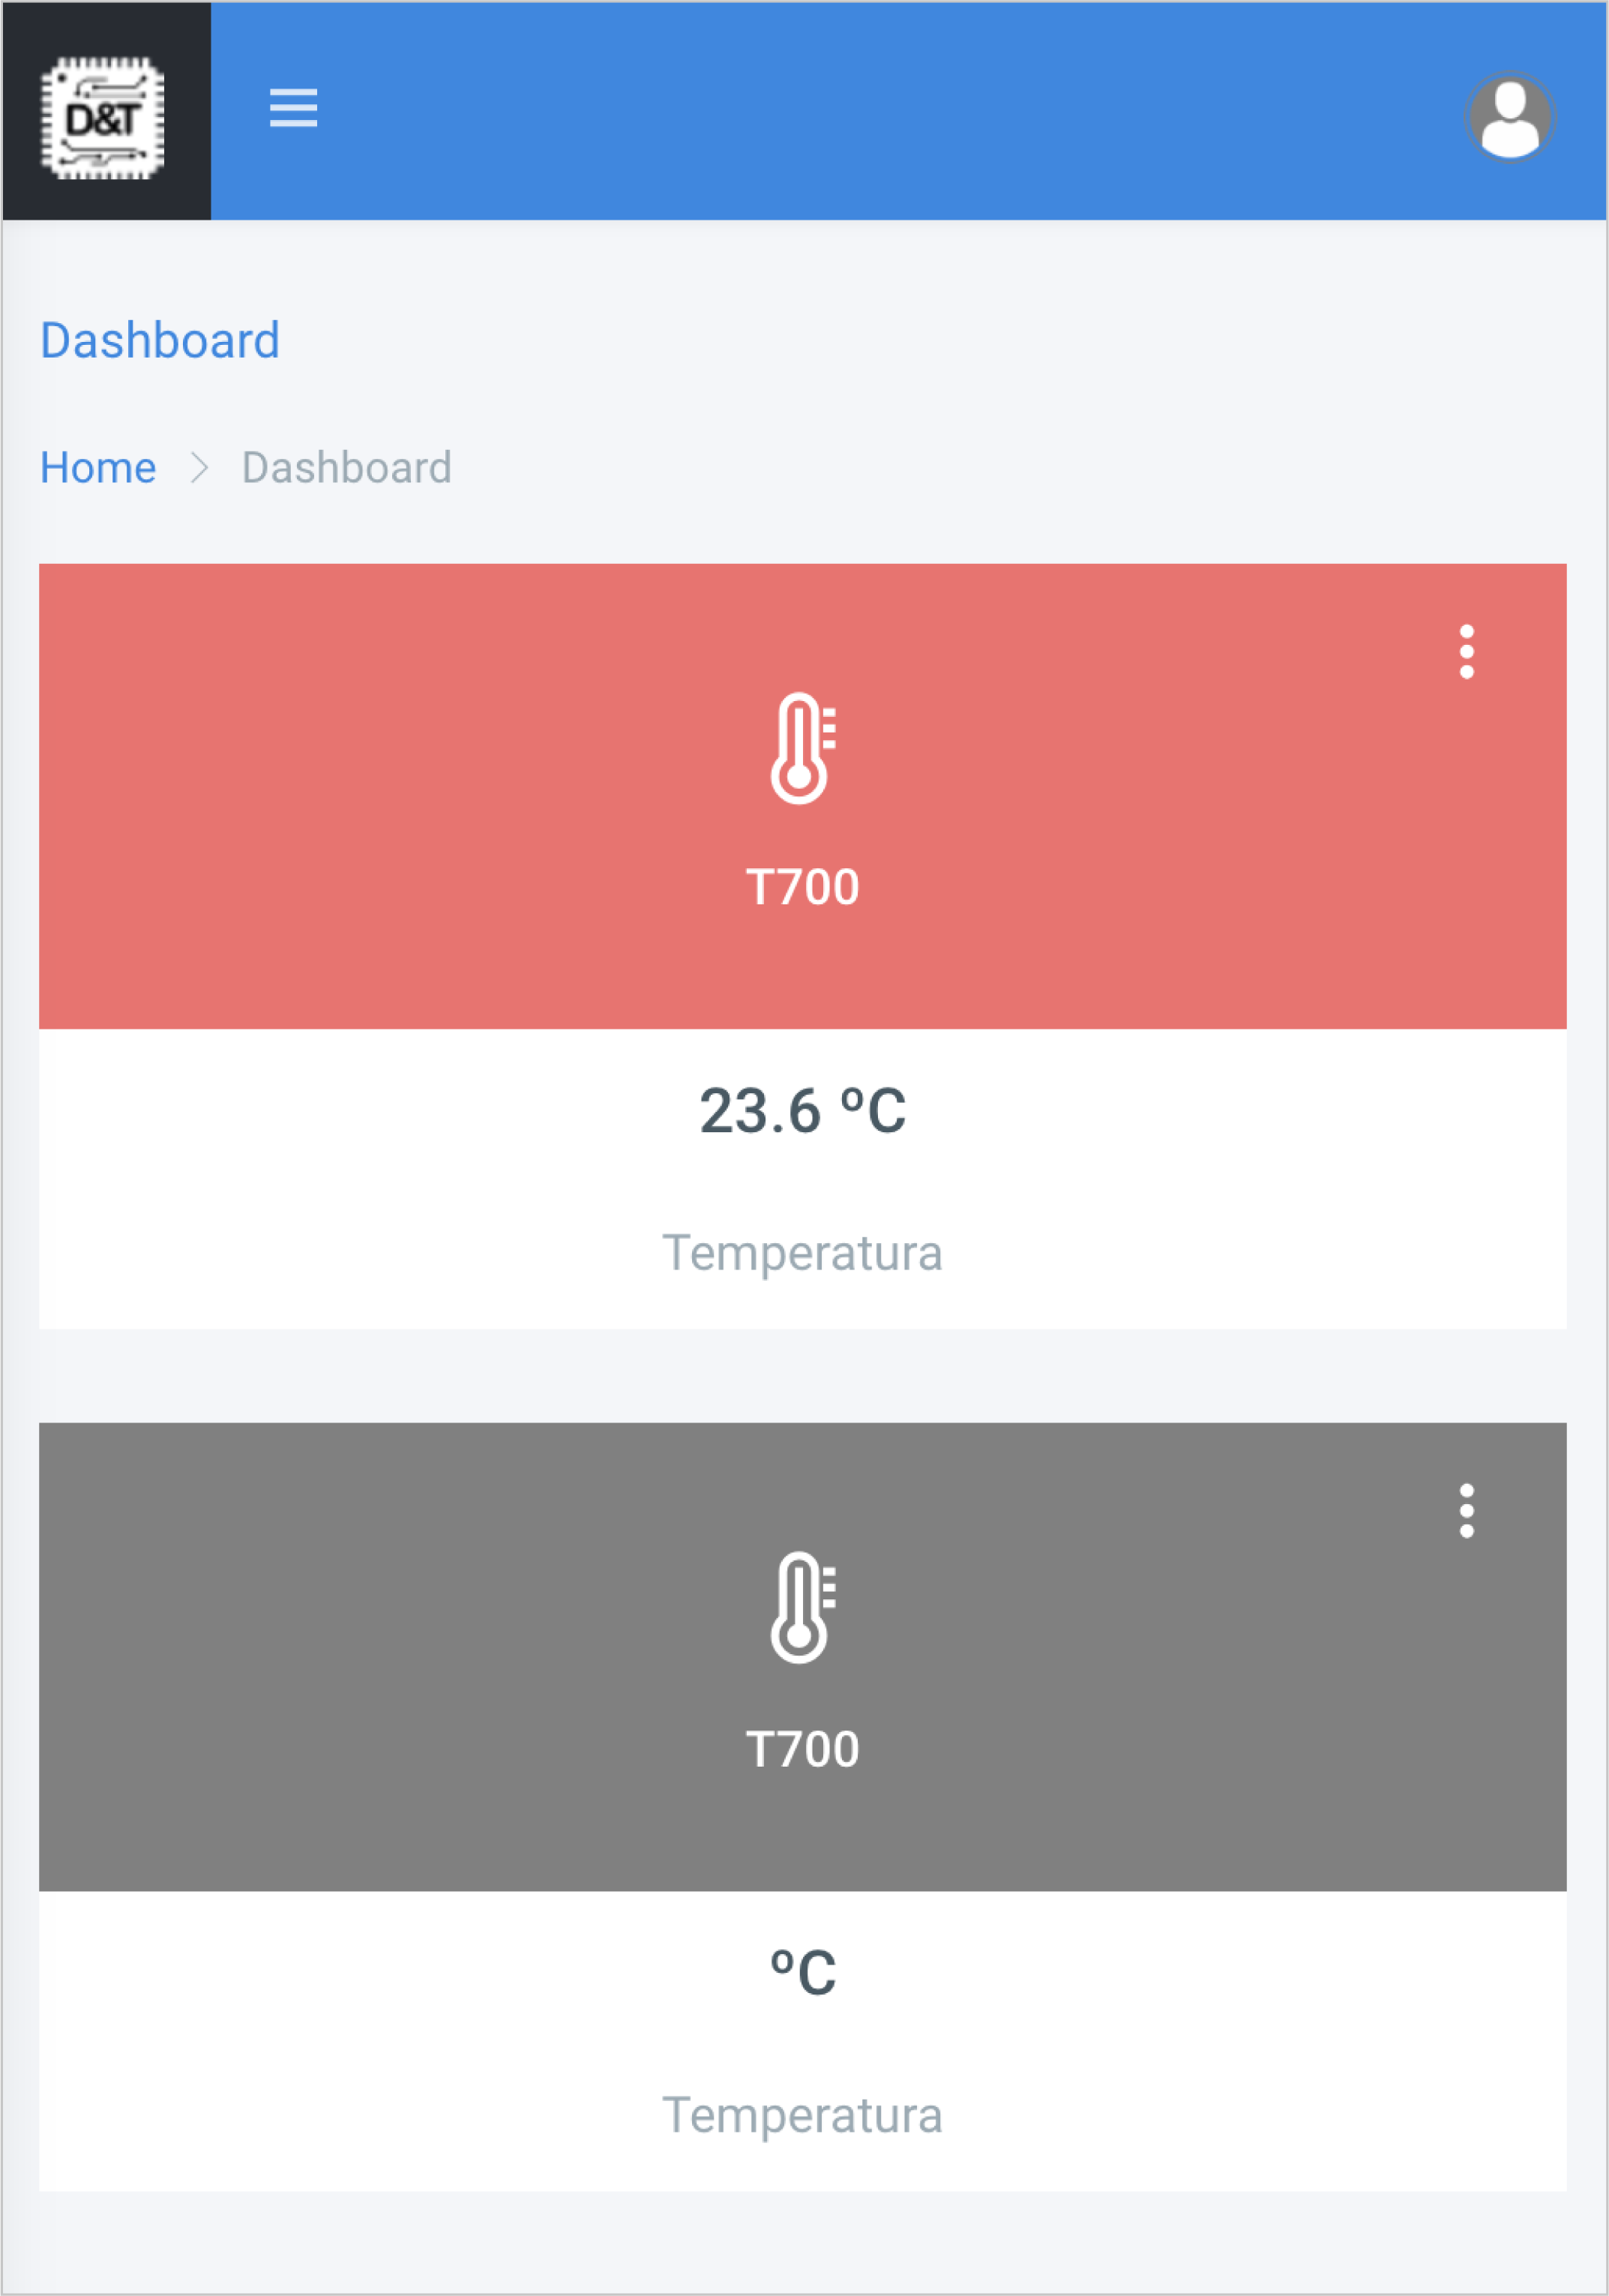
\includegraphics[scale=.20]{./Figures/pantalla-celu.png}
	\caption[Pantalla adaptada a celulares]{Ilustración de pantalla principal adaptada a celulares.}
	\label{fig:pantalla-celu}
\end{figure}


\section{Implementación y configuración de Nginx}

Para la implementación de Nginx en un servidor con sistema operativo Linux como el de este trabajo,  se debe instalarlo con el comando que se muestra en el código \ref{cod:nginx-install}. 

\begin{lstlisting}[label=cod:nginx-install,caption=Instalación de Nginx en servidor con sistema operativo Linux.] 

// Instalacion de Nginx
sudo apt install nginx

// Aplicar ajustes al firewall

sudo ufw app list

sudo ufw allow 'Nginx HTTP'

// Comprobar que Nginx funcione en el servidor
systemctl status nginx

\end{lstlisting} 

Para la configuración de Nginx en el servidor se deben tener en cuenta los siguientes archivos y directorios y como cada uno influye en el funcionamiento:

\begin{itemize}
	\item /etc/nginx: directorio de configuración de Nginx. En él se encuentran todos los archivos de configuración de Nginx.
	
	\item /etc/nginx/nginx.conf: archivo de configuración principal de Nginx. Esto se puede modificar para realizar cambios en la configuración general de Nginx.
	
	\item /etc/nginx/sites-available/: directorio en el que se pueden guardar bloques de servidor por sitio. Nginx no utilizará los archivos de configuración de este directorio a menos que estén vinculados al directorio sites-enabled. Normalmente, toda la configuración del bloque de servidor se realiza en este directorio y luego se habilita estableciendo un vínculo con el otro directorio.
	
	\item /etc/nginx/sites-enabled/: directorio en el que se almacenan los bloques de servidor habilitados por sitio. Normalmente, estos se crean estableciendo vínculos con los archivos de configuración del directorio sites-available.

	\item /etc/nginx/snippets: este directorio contiene fragmentos de configuración que pueden incluirse en otras partes de la configuración de Nginx. Los segmentos de configuración potencialmente repetibles reúnen las condiciones para la conversión a fragmentos.
\end{itemize}

Los dominios utilizados para este trabajo son:

\begin{itemize}
	\item frontend: \url{https://cloud.dytsoluciones.com.ar}.
	
	\item backend: \url{https://api.cloud.dytsoluciones.com.ar}.
\end{itemize}

La configuración para el frontend se realizó siguiendo los pasos del código \ref{cod:nginx-config}.

\begin{lstlisting}[label=cod:nginx-config,caption=Configuración de Nginx en servidor con sistema operativo Linux.] 

// Se crea el directorio con el nombre de dominio utilizado
sudo mkdir -p /var/www/cloud.dytsoluciones.com.ar/html

//Se asigna la propiedad del directorio con la variable de entorno $USER
sudo chown -R $USER:$USER /var/www/cloud.dytsoluciones.com.ar/html

// Para que Nginx pueda utilizar las directivas correcctas se crea un archivo de configuracion predeterminado. 

sudo nano /etc/nginx/sites-available/cloud.dytsoluciones.com.ar

// Se crea el enlace entre el archivo de configuracion y el directorio sites-enabled.
sudo ln -s /etc/nginx/sites-available/cloud.dytsoluciones.com.ar/ /etc/nginx/cloud.dytsoluciones.com.ar/

//Una vez finalizada la configuracion se reinicia el servicio
sudo systemctl restart nginx
\end{lstlisting} 


% Chapter Template

\chapter{Ensayos y Resultados} % Main chapter title
\label{Chapter4} % Change X to a consecutive number; for referencing this chapter elsewhere, use \ref{ChapterX}

En este capítulo se detallan los resultados esperados y obtenidos sobre etapas puntuales en el trabajo. También se indican las herramientas y metodología
empleadas en cada caso. Finalmente se expone el caso de uso completo integrando todos los componentes que lo componen.



%----------------------------------------------------------------------------------------
%	SECTION 1
%----------------------------------------------------------------------------------------

\section{Pruebas unitarias}

Las pruebas unitarias o \textit{unit testing} son una forma de comprobar que un fragmento de código funciona correctamente. Para este trabajo se programó un \textit{script} utilizando  shUnit2 \citep{WEBSITE:44}, para automatizar diferentes pruebas en la conexión con el broker MQTT.  

Las pruebas unitarias en el backend fueron realizadas teniendo en cuenta las etapas de desarrollo del proyecto y así poder asegurar que en la implementación del frontend no haya problemas en las respuestas a las diferentes consultas.

Por otro lado, se utilizó la herramienta de \textit{testing} que se incluye en Angular para realizar pruebas de la partes más importantes del frontend. 



%----------------------------------------------------------------------------------------
%	Integridad MQTT
%----------------------------------------------------------------------------------------

\subsection{Pruebas de integridad del broker MQTT}

Para hacer pruebas de integridad en el broker MQTT, se instaló shUnit2 y en un \textit{script} se programaron las diferentes pruebas para verificar si la conexión de clientes con el broker MQTT es segura o bien tiene fallas de seguridad. Estas pruebas automatizadas se realizaron mientras se cursaba la materia Ciberseguridad en Internet de las Cosas. 

En el código \ref{cod:script-mqtt} se muestran las diferentes funciones de testeo que se incluyeron en el script. La función de cada una es lograr publicar un mensaje en el broker teniendo en cuenta diferentes etapas de autenticación. 

\begin{lstlisting}[label=cod:script-mqtt,caption=Script para testing de integridad y seguridad de broker MQTT.] 

#! /bin/sh

########################################################################
#	Test para saber si un cliente sin credenciales 
#	puede conectarse - Envio de mensaje prueba_test
########################################################################
testClienteAnonimo(){
 VALUE=$(mosquitto_pub -p 8883 -m prueba_test -t /test -d | grep -o 'PUBLISH') 	
 assertFalse "$VALUE" "PUBLISH"
}

########################################################################
#	Test para saber si un cliente con solo usuario 
#	puede conectarse
########################################################################
testClienteConUsuario(){
 VALUE=$(mosquitto_pub -p 8883 -h localhost -u carlos -m hello -t /test -d | grep -o 'PUBLISH') 
 assertFalse "$VALUE" "PUBLISH"
}


########################################################################
#	Test para saber si un cliente con solo usuario 
#	y password puede conectarse
########################################################################
testClienteConUserYPass(){
 VALUE=$(mosquitto_pub -p 8883 -h localhost -u carlos -P carlos -m hello -t /test -d | grep -o 'PUBLISH') 
 assertFalse "$VALUE" "PUBLISH"
}


########################################################################
#	Test para saber si un cliente puede conectarse
#	con certificados validos
########################################################################
testClienteTLS(){
 VALUE=$(mosquitto_pub -p 8883 --cafile ../ca/ca.crt --cert ../client/client.crt --key ../client/client.key -h localhost -u carlos -P cars -m hello -t /test -d | grep -o 'PUBLISH') 	
 assertEquals "$VALUE" "PUBLISH"
}

\end{lstlisting}

En la tabla \ref{tab:test-mqtt} se describen los tests realizados.

\begin{table}[h]
	\centering
	\caption[Comandos utilizados en MongoDB]{Comandos más utilizados para el manejo de base de datos desarrollada en MongoDB.}
	\begin{tabular}{l p{4.5cm} c }    
		\toprule
		\textbf{Test} 	 										& \textbf{Descripción} 																						& \textbf{Resultado esperado}\\
		\midrule
	
		testClienteAnonimo()			& Verificar si un cliente sin credenciales puede conectarse al broker.    				& Error de conexión\\		
		
		testClienteConUsuario() 			& Verificar si un cliente con nombre de usuario y sin password puede conectarse al broker.    				& Error de conexión\\		
		
		testClienteConUserYPass() 		& Verificar si un cliente con nombre de usuario y password puede conectarse al broker.    				& Error de conexión\\	
		
		testClienteTLS()						& Verificar si un cliente con nombre de usuario y password y certificados puede conectarse al broker.    				& Publicación exitosa\\	
		\bottomrule
		\hline
	\end{tabular}
	\label{tab:test-mqtt}
\end{table}

\pagebreak

Los resultados obtenidos pueden observarse en la figura \ref{fig:mqtt-test}.

\begin{figure}[htpb]
	\centering
	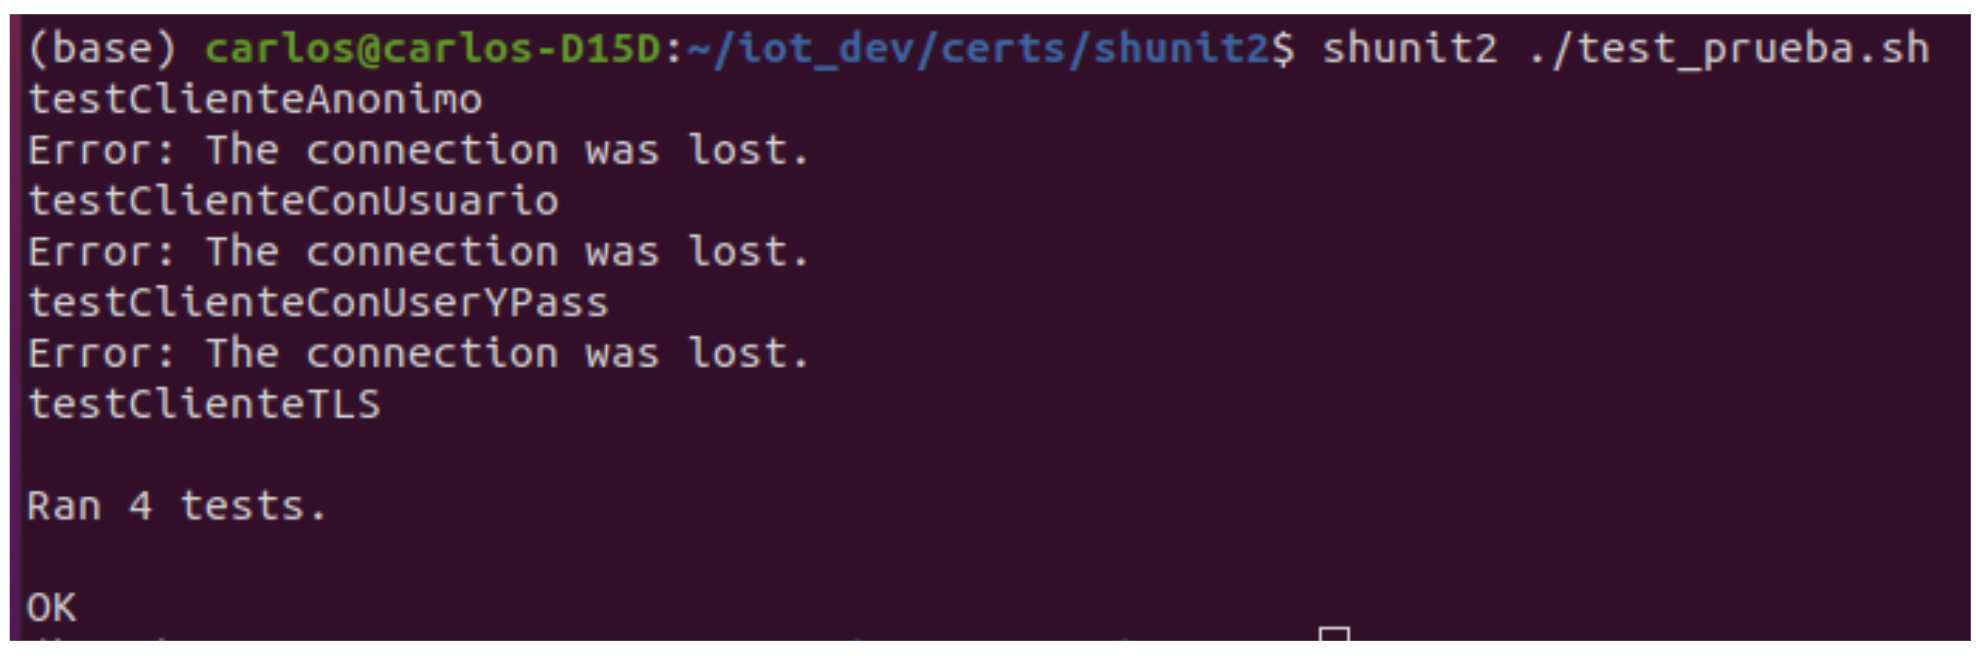
\includegraphics[scale=.35]{./Figures/mqtt-test.png}
	\caption[Testing broker MQTT]{Test de integridad y seguridad del broker MQTT.}
	\label{fig:mqtt-test}
\end{figure}



%----------------------------------------------------------------------------------------
%	Unit Tests
%----------------------------------------------------------------------------------------

\subsection{Pruebas unitarias de funciones del backend}
\label{backend-unit}
Para las pruebas unitarias de las funciones del backend se utilizó el software Postman \citep{WEBSITE:45}, el cual permitió realizar las pruebas de todas las funciones definidas en el backend desde un único sitio. 

En la figura \ref{fig:postman-backend} pueden observarse las carpetas de cada sección de funciones utilizadas en el backend. 

\begin{figure}[htpb]
	\centering
	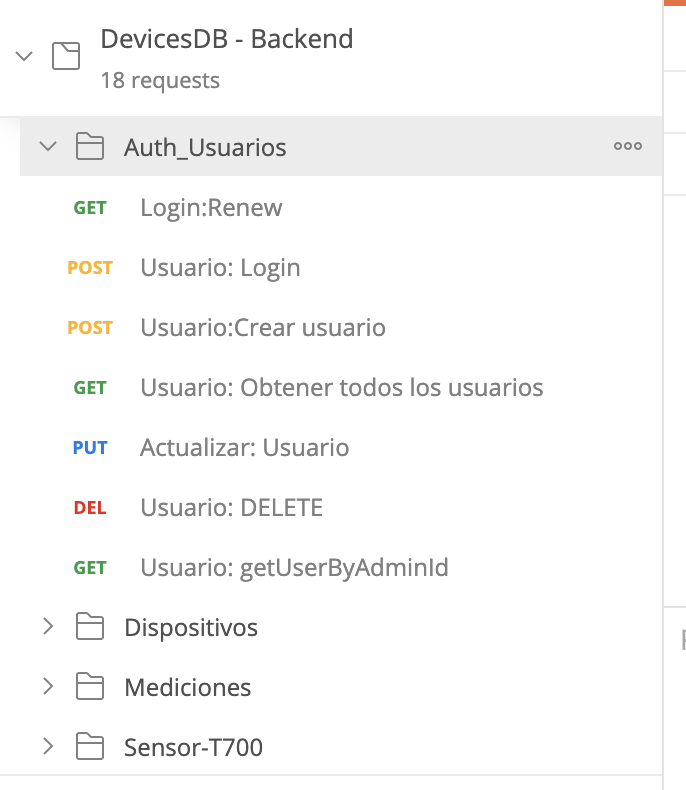
\includegraphics[scale=.56]{./Figures/backend-postman.png}
	\caption[Carpetas de funciones para testing en Postman]{Carpeta con peticiones http para testing de backend en Postman.}
	\label{fig:postman-backend}
\end{figure}

\newpage

Para hacer una petición http al backend, se seleccionó la opción de login de usuario donde se realizó una petición POST pasando como parámetros en el cuerpo del mensaje el email y password como se observa en la figura \ref{fig:postman-login}.

\begin{figure}[htpb]
	\centering
	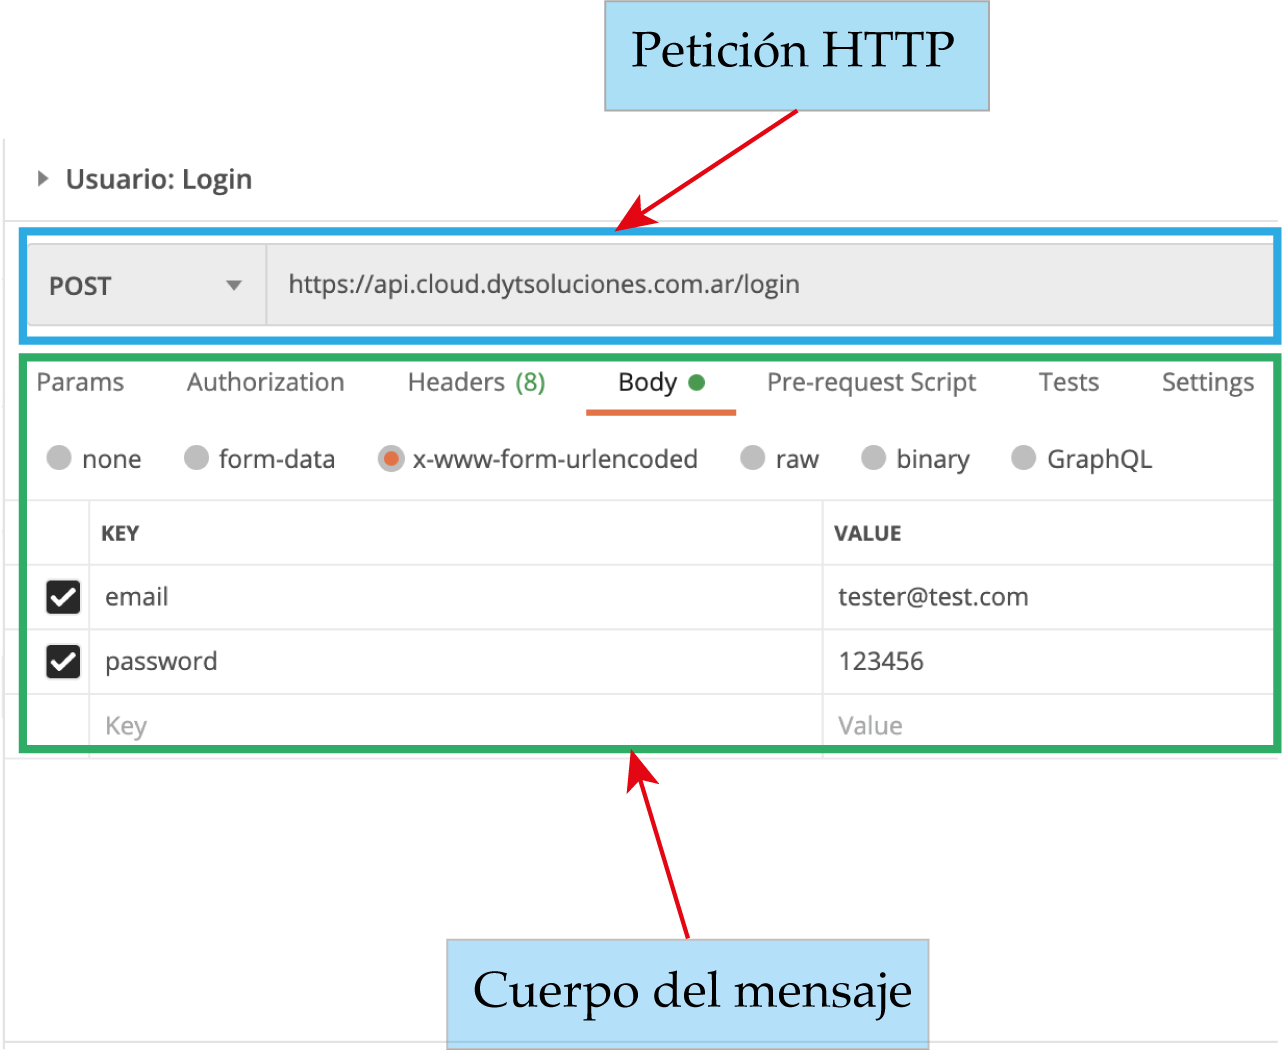
\includegraphics[scale=1.1]{./Figures/postman-login.png}
	\caption[Petición HTTP a función de login de usuarios en Postman]{Ilustración de entorno Postman para hacer una petición POST a la función login de usuario del backend.}
	\label{fig:postman-login}
\end{figure}

\pagebreak
La respuesta a esta petición espera un mensaje en formato JSON con el estado. En caso de ser correcta, se espera un código 200 y además un \textit{token} de acceso para las funciones que lo requieren.  En la figura \ref{fig:login-response} se puede observar la respuesta a la petición POST para el login de usuario.

\begin{figure}[htpb]
	\centering
	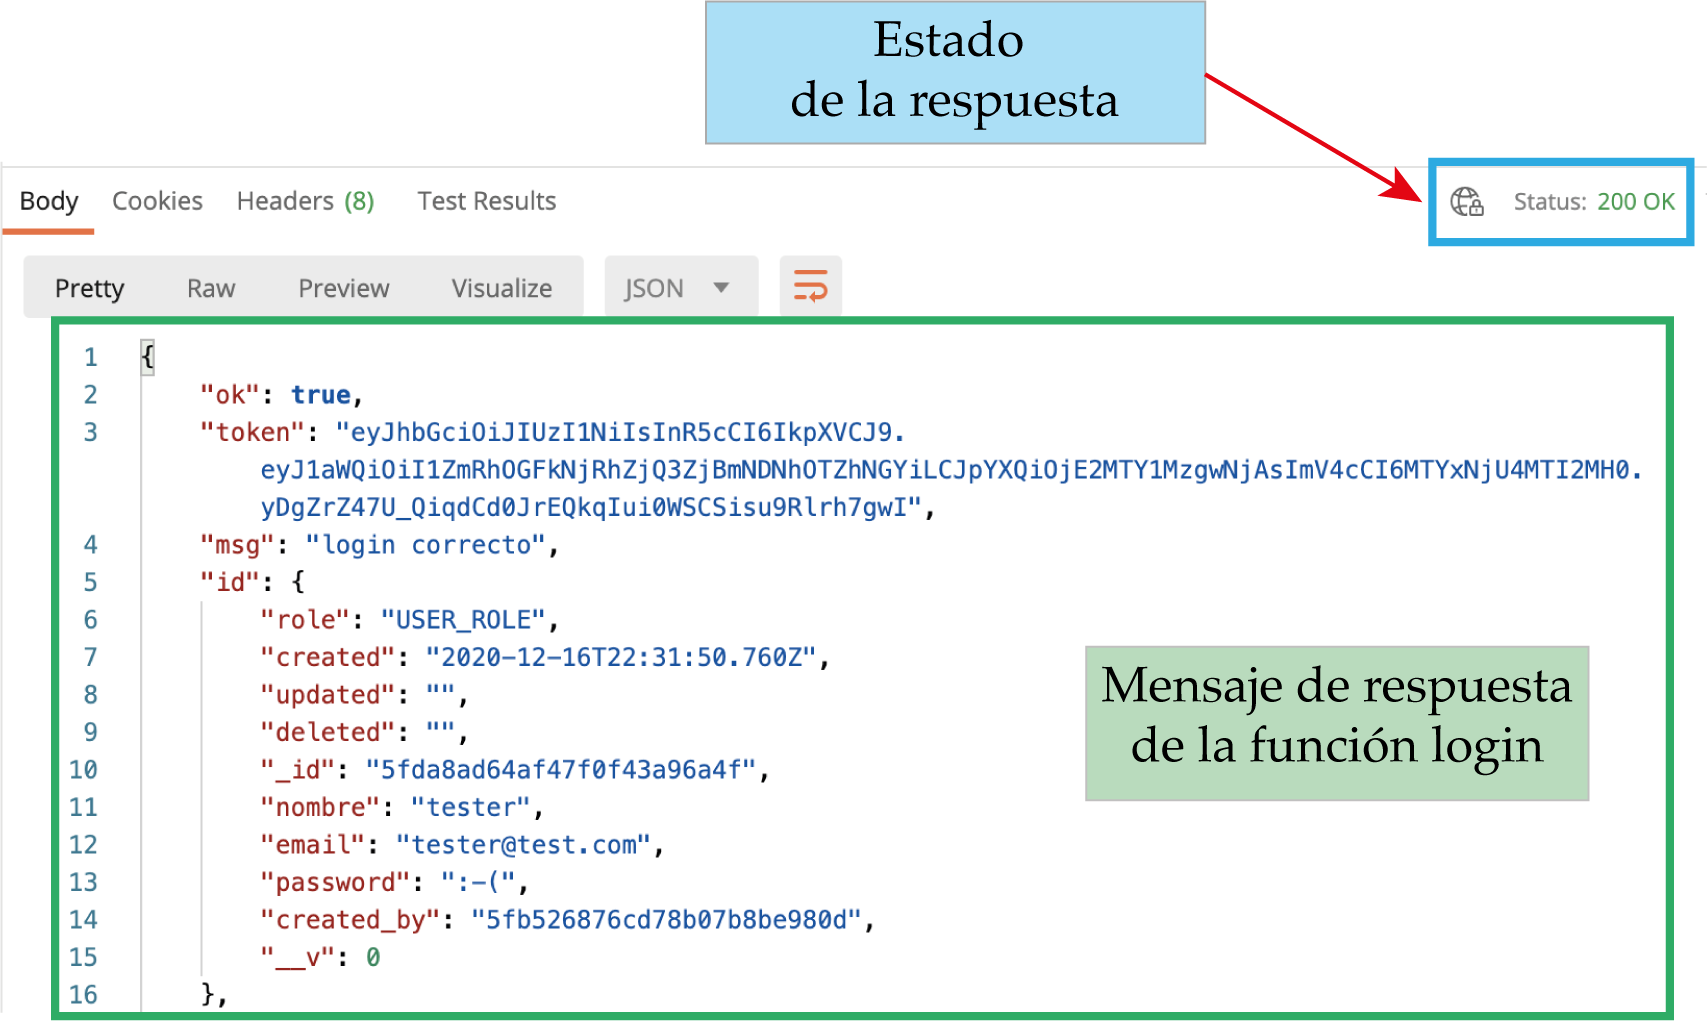
\includegraphics[scale=0.90]{./Figures/login-response.png}
	\caption[Respuesta a petición de login desde Postman]{Ilustración de respuesta del backend a la petición POST de login de usuario en Postman.}
	\label{fig:login-response}
\end{figure}

\pagebreak
Luego del test de login de usuario y de obtener un token, se realizó un test de acceso a funciones del backend que tienen como condición que el usuario envíe un token válido para poder acceder a las respuestas de las mismas. 

El test consistió en realizar la petición con un token inválido esperando un estado de error en su respuesta como se muestra en la figura \ref{fig:not-token-dev}.  

\begin{figure}[htpb]
	\centering
	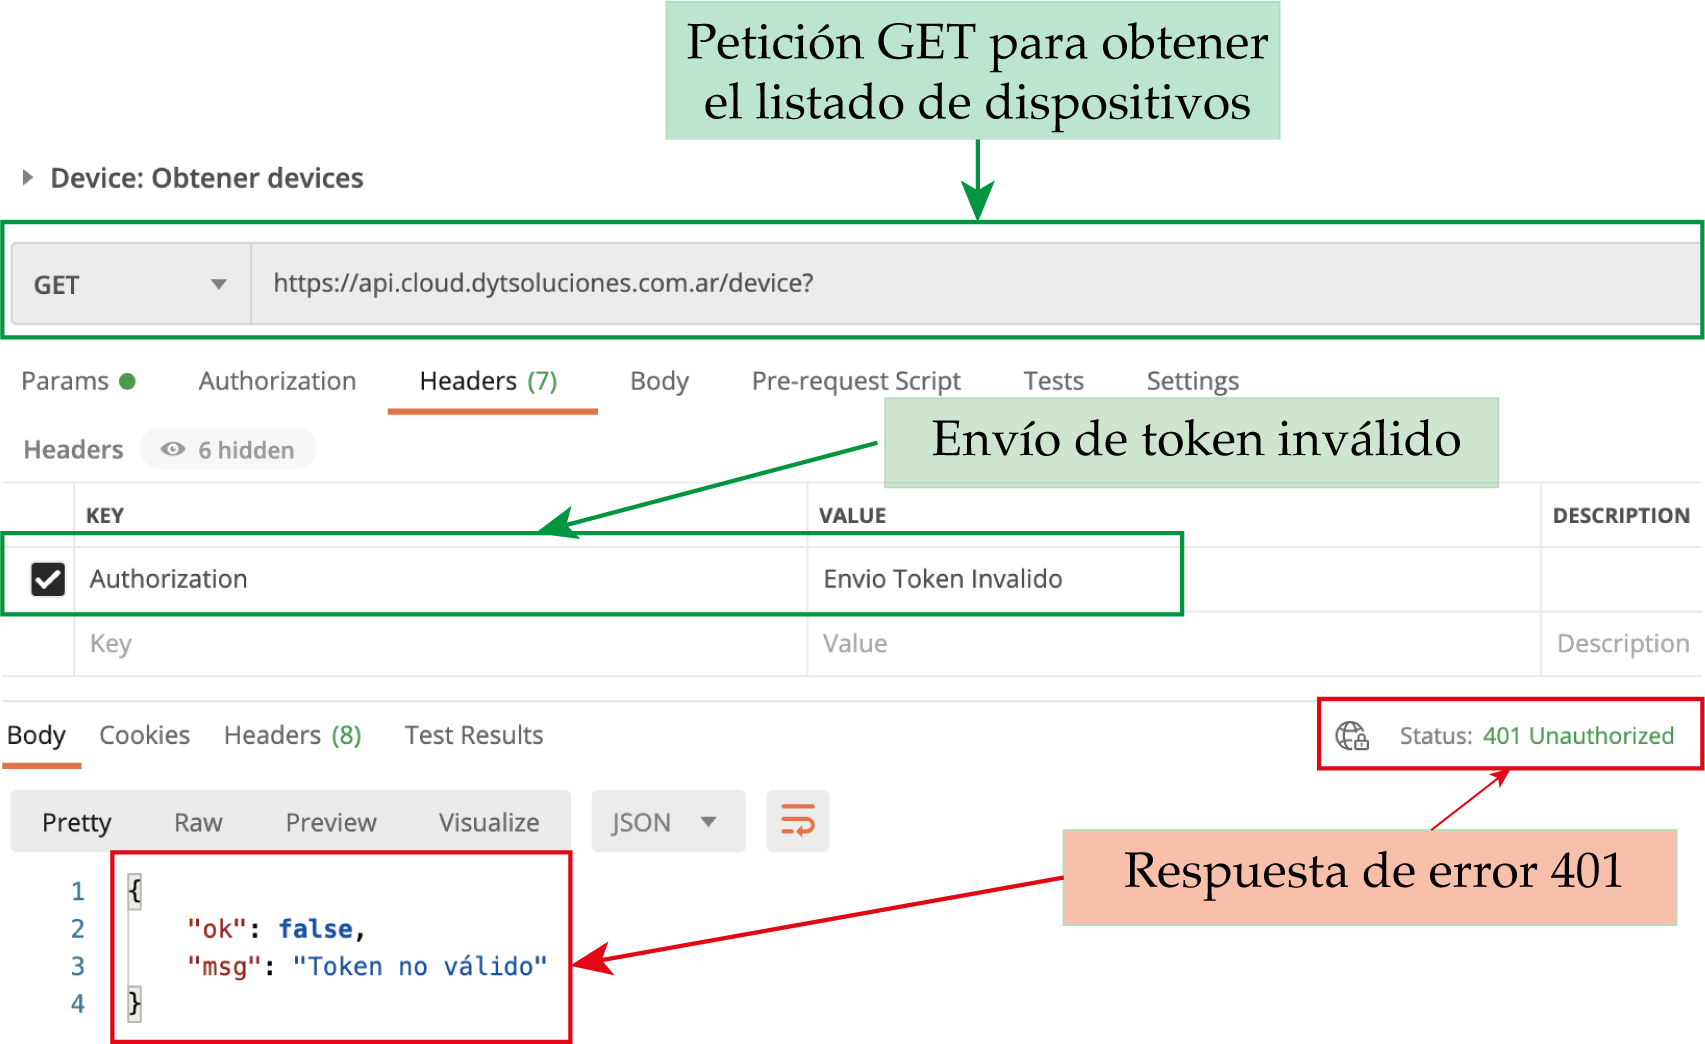
\includegraphics[scale=.90]{./Figures/devices-no-token.png}
	\caption[Respuesta a petición de dispositivos con token inválido]{Ilustración de respuesta del backend a la petición GET de dispositivos con token inválido.}
	\label{fig:not-token-dev}
\end{figure}

\newpage

Por otro lado, en la figura  \ref{fig:valid-token-dev} se realizó la petición de dispositivos al servidor utilizando el token válido adquirido en el login de usuario.



\begin{figure}[htpb]
	\centering
	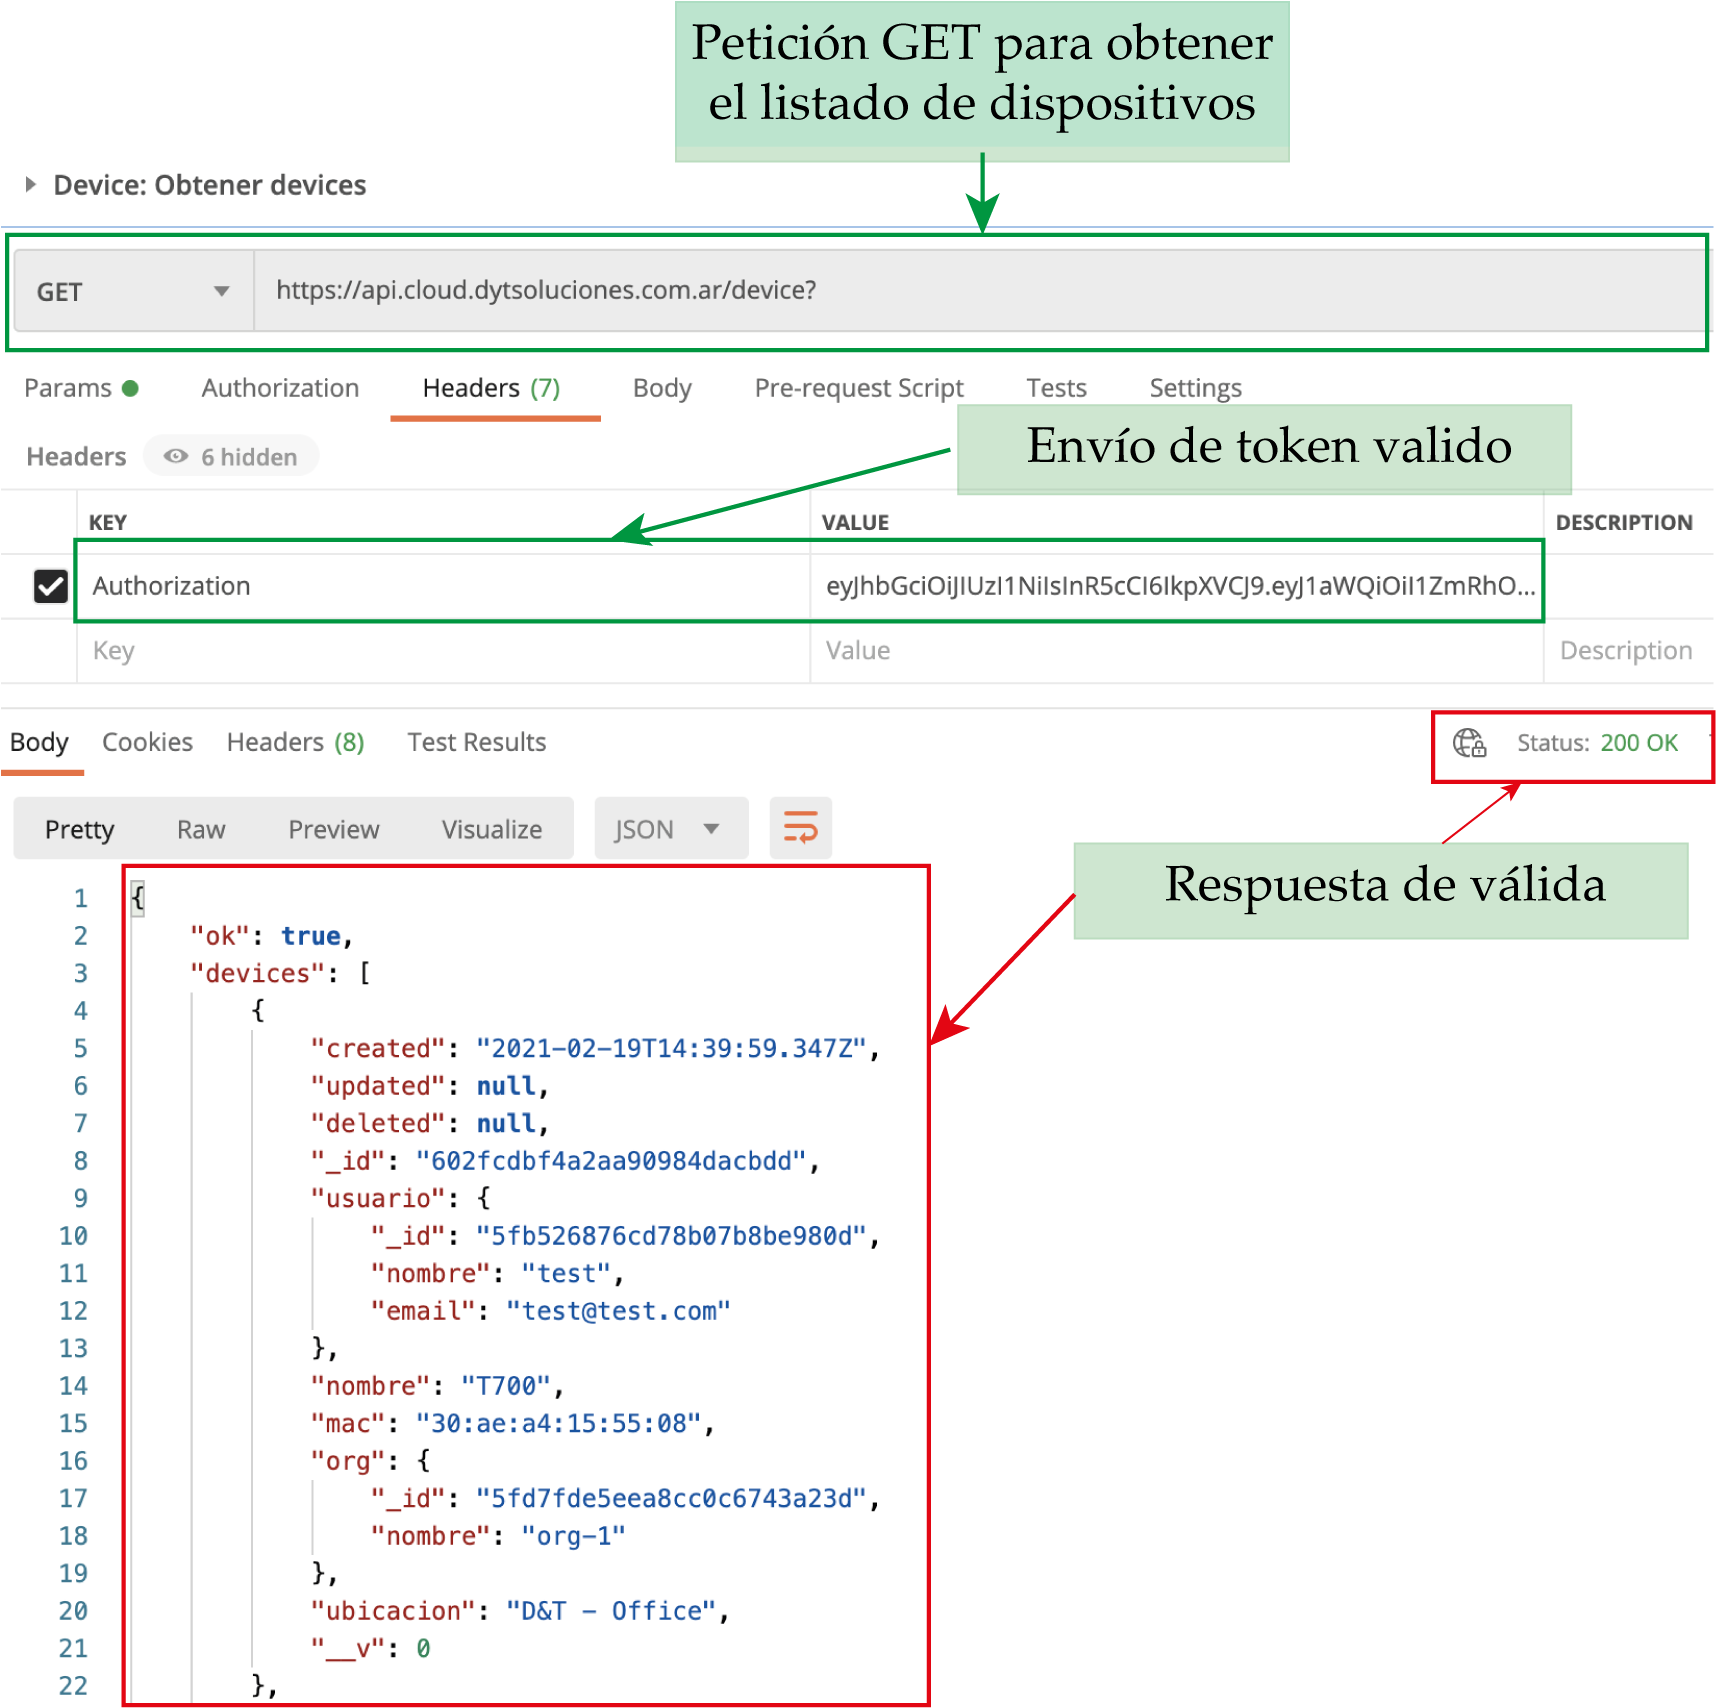
\includegraphics[scale=.90]{./Figures/devices-valid-token.png}
	\caption[Respuesta a petición de dispositivos con token válido]{Ilustración de respuesta del backend a la petición GET de dispositivos con token válido.}
	\label{fig:valid-token-dev}
\end{figure}



%----------------------------------------------------------------------------------------
%	Integration Tests
%----------------------------------------------------------------------------------------

\section{Ensayos de integración}

El objetivo de las pruebas de integración es verificar el correcto funcionamiento entre los distintos componentes del sistema una vez que han sido probados unitariamente.  El fin es comprobar que interactúan correctamente a través de sus interfaces, tanto internas como externas, cubren las funcionalidades establecidas y se ajustan a los requisitos no funcionales especificados en las verificaciones correspondientes.


Para las pruebas de todo el sistema se utilizó la herramienta Cypress \citep{WEBSITE:46} que es un framework que incluye librerías de aserciones, mocks y pruebas e2e \citep{WEBSITE:48} automáticas. Esta herramienta está diseñada especialmente para manejar \textit{frameworks} de Javascript como Angular, Vue, ReactNative, entre otros.

Para la instalación de Cypress sobre Angular, se utilizó npm \citep{WEBSITE:47} y en el código \ref{cod:cmd-cypress} se puede observar el comando utilizado. 

\begin{lstlisting}[label=cod:cmd-cypress,caption=Comando de instalación de Cypress en Angular.] 

npm install cypress --save-dev
\end{lstlisting}

En la figura \ref{fig:cypress-install} se observa la integración de Cypress al archivo de dependencias del desarrollo de Angular  y además la creación de dos archivos para el testeo del sistema en la carpeta de integración. 

\begin{figure}[htpb]
	\centering
	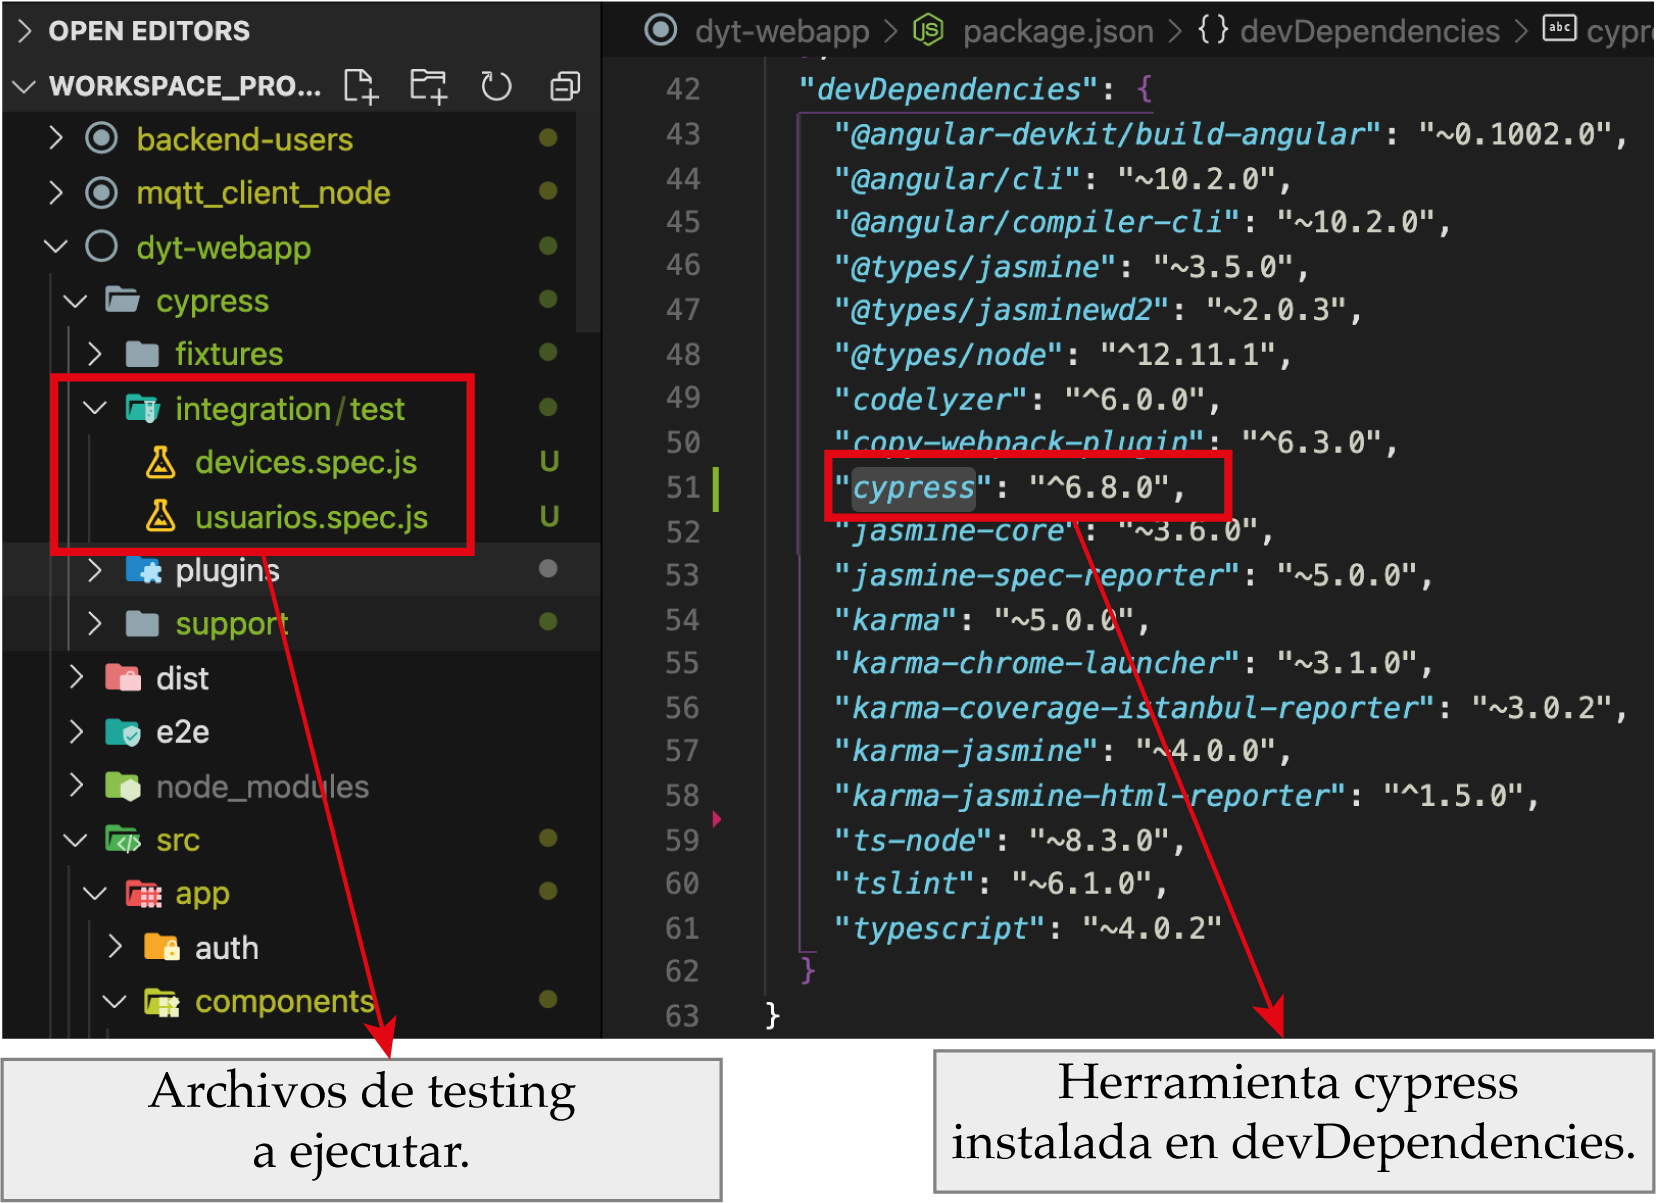
\includegraphics[scale=.9]{./Figures/cypress-install.png}
	\caption[Archivos de instalación de Cypress]{Ilustración archivos de testing generados en carpeta \textit{integration/test} y herramienta instalada en dependencias de desarrollo.}
	\label{fig:cypress-install}
\end{figure}


%----------------------------------------------------------------------------------------
%	Usuarios Integration
%----------------------------------------------------------------------------------------

\subsection{Pruebas de integridad en login de usuarios}
\label{login-tests}
Esta prueba consiste en automatizar los test unitarios que se realizaron en la sección \ref{backend-unit}. Con el uso de Cypress se pudo simular el comportamiento de la pantalla de login de la plataforma web con el usuario, pudiendo observar para cada test, la respuesta que esta pantalla informa al usuario.

En el código \ref{cod:test-login-cypress} se muestra la implementación para los tests que se realizaron en la pantalla de login.

\begin{lstlisting}[label=cod:test-login-cypress,caption=Código de implementación para tests realizados en la pantalla de login de la plataforma web.] 

/// <reference types="cypress" />

context('Test de pagina de login', () => {
  // Antes de cada test, debe visitar la pantalla de login.
  beforeEach(() => {
    cy.visit('http://localhost:4200');
  })


  it('Si el campo email del formulario esta vacio, debe avisar al usuario.', ()=>{
    cy.get('.m-t-40 > .col-xs-12 > .form-control')
      .type('none@test.com').should('have.value', 'none@test.com')
    
    cy.get(':nth-child(3) > .col-xs-12 > .form-control')
      .type('123456').should('have.value', '123456')

    cy.get('#loginform')
      .submit()
      .next()

    cy.get('#swal2-content')
      .contains('Email no encontrado')
  
  });

  it('Si el email ingresado no pertenece a un usuario registrado debe dar un aviso. ', ()=>{
    cy.get('.m-t-40 > .col-xs-12 > .form-control')
      .type('test@test.com').should('have.value', 'test@test.com')
    
    cy.get(':nth-child(3) > .col-xs-12 > .form-control')
      .type('malPass').should('have.value', 'malPass')

    cy.get('#loginform')
      .submit()
      .next()

    cy.get('#swal2-content')
      .contains('Credenciales incorrectas')
  
  });

  it('Si el email ingresado tiene un formato incorrecto, debe avisar al usuario.  ', ()=>{
    cy.get('.m-t-40 > .col-xs-12 > .form-control')
      .type('none!test.com').should('have.value', 'none!test.com')
    
    cy.get(':nth-child(3) > .col-xs-12 > .form-control')
      .type('123456').should('have.value', '123456')

    cy.get('#loginform')
      .submit()
      .next()

      cy.get('.col > p')
        .contains('Debe especificar un email valido')
  
  });

  it('Si el campo del password del formulario esta vacio, debe avisar al usuario.  ', ()=>{
    cy.get('.m-t-40 > .col-xs-12 > .form-control')
      .type('none@test.com').should('have.value', 'none@test.com')
    
    cy.get('#loginform')
      .submit()
      .next()

    cy.get('.col > p')
    .contains('Debe especificar un password')
      
  });

  it('Al ingresar un email y password registrado en el sistema, la pagina debe navegar hacia la ruta /dashboard. ', ()=>{
    cy.get('.m-t-40 > .col-xs-12 > .form-control')
      .type('test@test.com').should('have.value', 'test@test.com')
    
    cy.get(':nth-child(3) > .col-xs-12 > .form-control')
      .type('123456').should('have.value', '123456')

    cy.get('#loginform')
      .submit()
      .next()

    cy.contains('Dashboard')
  
  });

  it('Al realizar el login de un usuario registrado, se debe almacenar el token en el localStorage. ', ()=>{
    cy.get('.m-t-40 > .col-xs-12 > .form-control')
      .type('test@test.com').should('have.value', 'test@test.com')
    
    cy.get(':nth-child(3) > .col-xs-12 > .form-control')
      .type('123456').should('have.value', '123456')

    cy.get('#loginform')
      .submit()
      .next()

    cy.window()
      .its("localStorage")
      .invoke("getItem", "token")
      .should("exist");
  
  });
  
});

\end{lstlisting}


La descripción y resultados de los tests realizados fueron los que se detallan en la tabla \ref{tab:test-cypress-login}.

\begin{table}[h]
	\centering
	\caption[Test de login utilizando Cypress]{Diferentes test automáticos en pantalla login de usuario de la plataforma web utilizando Cypress.}
	\begin{tabular}{p{4cm} p{4cm} p{4cm}}    
		\toprule
		\textbf{Test Cypress }  		& \textbf{Descripción}	& \textbf{Resultado}\\
		\midrule
	
		Si el campo email del formulario está vacío, debe avisar al usuario. 			& Presionar el botón login sin completar el campo email del formulario. 				& Mensaje informando al usuario que debe especificar un email válido. \\	
		
		Si el email ingresado no pertenece a un usuario registrado debe dar un aviso.	 			& Realizar el login con un email no registrado en el sistema. 				& Mensaje de error informando al usuario que el email no fue encontrado.\\	
		
		Si el email ingresado tiene un formato incorrecto, debe avisar al usuario.   & Realizar el login con un texto sin el símbolo \@ en el campo email del formulario.		& Mensaje informando al usuario que debe especificar un email válido.  \\
		
		Si el campo del password del formulario está vacío, debe avisar al usuario. 	 & Presionar el botón login sin completar el campo password del formulario.    & Mensaje informando al usuario que las credenciales son incorrectas.\\	
		
		  
		Al ingresar un email y password registrado en el sistema, la página debe navegar hacia la ruta /dashboard.   & Realizar el login con un email y password previamente registrado en el sistema.  & Visualización de la pantalla dashboard en la plataforma web.\\	
		
		Al realizar el login de un usuario registrado, se debe almacenar el \textit{token} en el localStorage. 		& Realizar el login con un email y password previamente registrado en el sistema y verificar si existe el item \textit{token} en el localStorage. 		& El \textit{token} existe en el localStorage del navegador web.\\	
		
		\bottomrule
		\hline
	\end{tabular}
	\label{tab:test-cypress-login}
\end{table}

\pagebreak

Es importante mencionar que no solamente se están automatizando los tests unitarios sino que además se están verificando los componentes HTML de la plataforma así como los datos alojados en la base de datos. Este tipo de tests también se conocen como e2e (\textit{end-to-end}) y replican el comportamiento de los usuarios con el software en un entorno de aplicación completo. Estas pruebas verifican que los flujos que sigue un usuario trabajen como se espera. En la figura \ref{fig:cypress-test-login} se pueden observar desde la interfaz de Cypress los resultados de los tests realizados.

\begin{figure}[htpb]
	\centering
	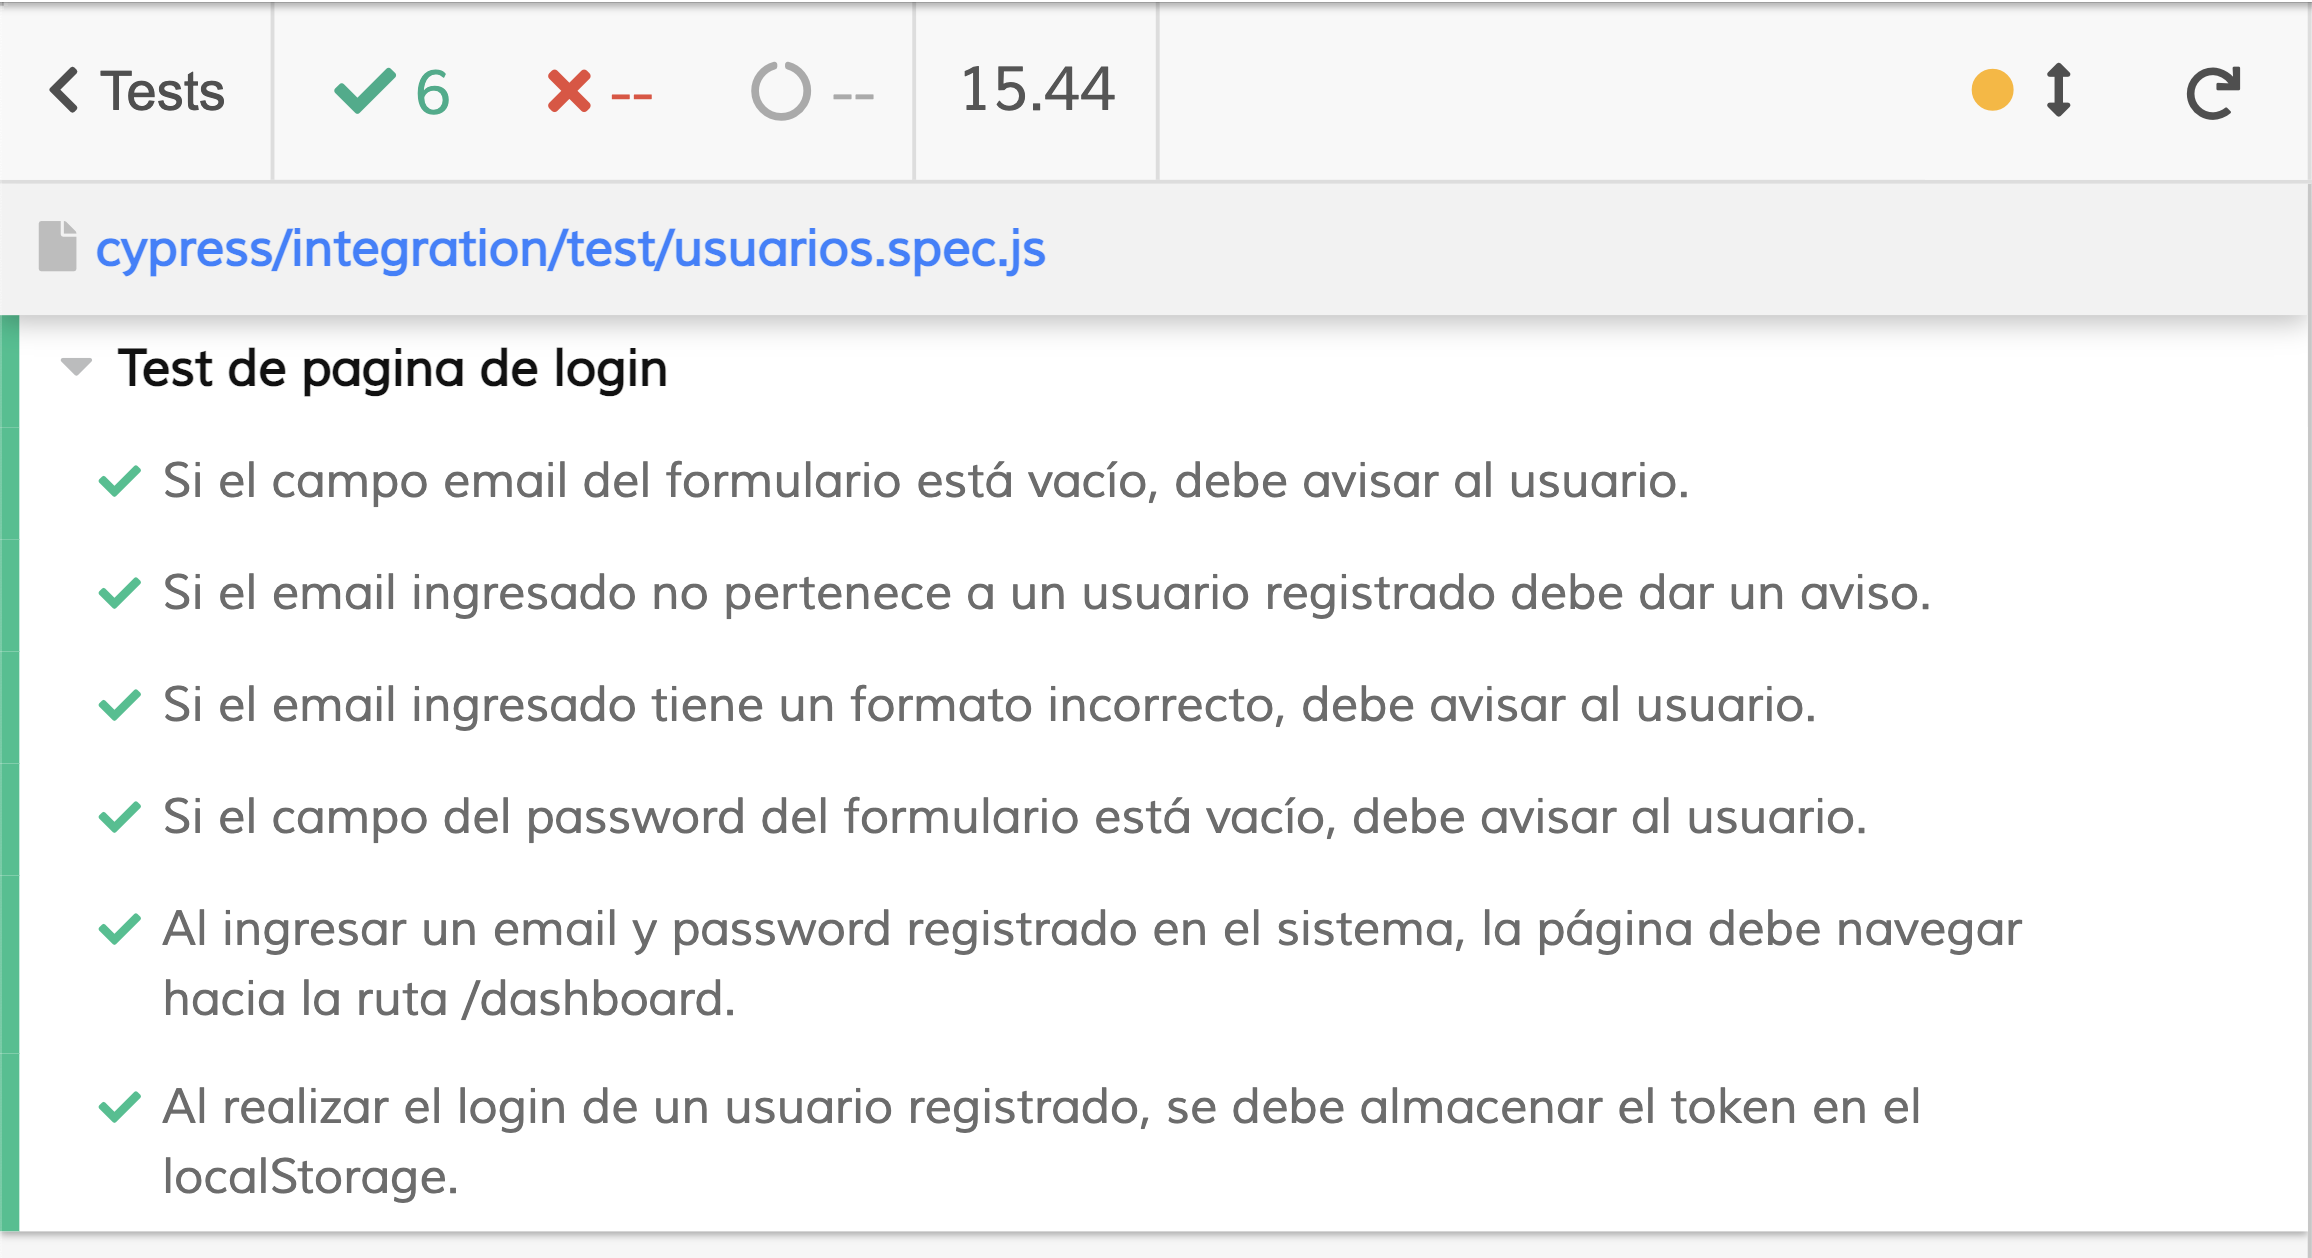
\includegraphics[scale=.30]{./Figures/test-login-cypress.png}
	\caption[Resultado de test de login de la plataforma web]{Ilustración del entorno web de Cypress con los resultados de los test realizados y verificados.}
	\label{fig:cypress-test-login}
\end{figure}

\pagebreak

%----------------------------------------------------------------------------------------
%	Devices Integration
%----------------------------------------------------------------------------------------

\subsection{Pruebas de integridad en dispositivos conectados}
\label{devs-cypress}


Al igual que la sección \ref{login-tests} mediante Cypress se realizaron los tests de integración para los dispositivos del sistema. Una condición a tener en cuenta cuando se realizaron estos tests fue que el usuario llamado test tiene al menos dos dispositivos en su cuenta.  

El código \ref{cod:test-devices-cypress} muestra la implementación de cada una de las pruebas realizadas. 

\begin{lstlisting}[label=cod:test-devices-cypress,caption=Código de implementación para tests realizados en la interacción de usuarios con dispositivos que se encuentran en el sistema.] 

/// <reference types="cypress" />


context('Test de Dispositivos', () => {
    
    Cypress.Commands.add('login', () => { 
        cy.request({
          method: 'POST',
          url: 'https://api.cloud.dytsoluciones.com.ar/login',
          body: {
              email: 'test@test.com',
              password: '123456',      
          }
        })
        .then((resp) => {
        
          window.localStorage.setItem('token', resp.body.token)
          
        })
    })

    // Antes de cada test, debe visitar la pantalla de login.
    beforeEach(() => {
        cy.login()  
    })

    it('En la pantalla del dashboard, deben mostrarse los dispositivos asociados al usuario que realizo el login.', ()=>{
        cy.visit('http://localhost:4200/dashboard');
        cy.contains('Dashboard');

        cy.get(':nth-child(1) > app-t700-sensor > .card > .row > :nth-child(1) > .social-widget > .soc-header')
            .should('exist');
      
    });

    it('Al navegar hacia la pantalla de dispositivos asignados al usuario, debe existir un listado de estos. ', ()=>{
        cy.visit('http://localhost:4200/dashboard/devices');
        cy.contains('Dispositivos')
        cy.get('tbody > tr > td').eq(0)
            .should('contain', 1)
    });

    it('En el dashboard si un dispositivo esta conectado, dl color de su componente no debe ser gris. ', ()=>{
        cy.visit('http://localhost:4200/dashboard');
        cy.contains('Dashboard')       
        cy.wait(10000)
        cy.get(':nth-child(1) > app-t700-sensor > .card > .row > :nth-child(1) > .social-widget > .soc-header', {timeout: 10000})
            .should('have.css', 'background-color', 'rgb(248, 108, 107)')
        
    });

});

\end{lstlisting}


Por otro lado en la tabla \ref{tab:test-cypress-devs} se puede observar la descripción de cada prueba y los resultados obtenidos pueden observarse en la figura \ref{fig:cypress-test-devs}. 
\pagebreak
\begin{table}[h]
	\centering
	\caption[Test de login utilizando Cypress]{Diferentes test automáticos en pantalla login de usuario de la plataforma web utilizando Cypress.}
	\begin{tabular}{p{4cm} p{4cm} p{4cm}}    
		\toprule
		\textbf{Test Cypress }  		& \textbf{Descripción}	& \textbf{Resultado}\\
		\midrule
	
		En la pantalla del \textit{dashboard}, deben mostrarse los dispositivos asociados al usuario que realizó el login.			& Al hacer un login de usuario, la página navega hacia el \textit{dashboart} y se verifica que exista al menos un dispositivo.				& Listado de dispositivos vinculados al usuario que realizó el login.\\	
		
		Al navegar hacia la pantalla de dispositivos asignados al usuario, debe existir un listado de estos. 	 			& Navegar hacia la pantalla /dashboard/devices, verificar que se listen los dispositivos asociados al usuario que realizó el login 				& El primer numero de la lista debe ser igual a uno, indicando que se carga el primer dispositivo.\\	
		
		En el \textit{dashboard} si un dispositivo está conectado, dl color de su componente no debe ser gris.   & Cargar la pagina del \textit{dashboard}, esperar diez segundos para testear si el color del componente del dispositivo cambió a un color diferente del gris indicando que está conectado.		& Se visualiza el cambio de color del componente que identifica a un dispositivo conectado al sistema. \\
		
		
		\bottomrule
		\hline
	\end{tabular}
\label{tab:test-cypress-devs}
\end{table}




\begin{figure}[htpb]
	\centering
	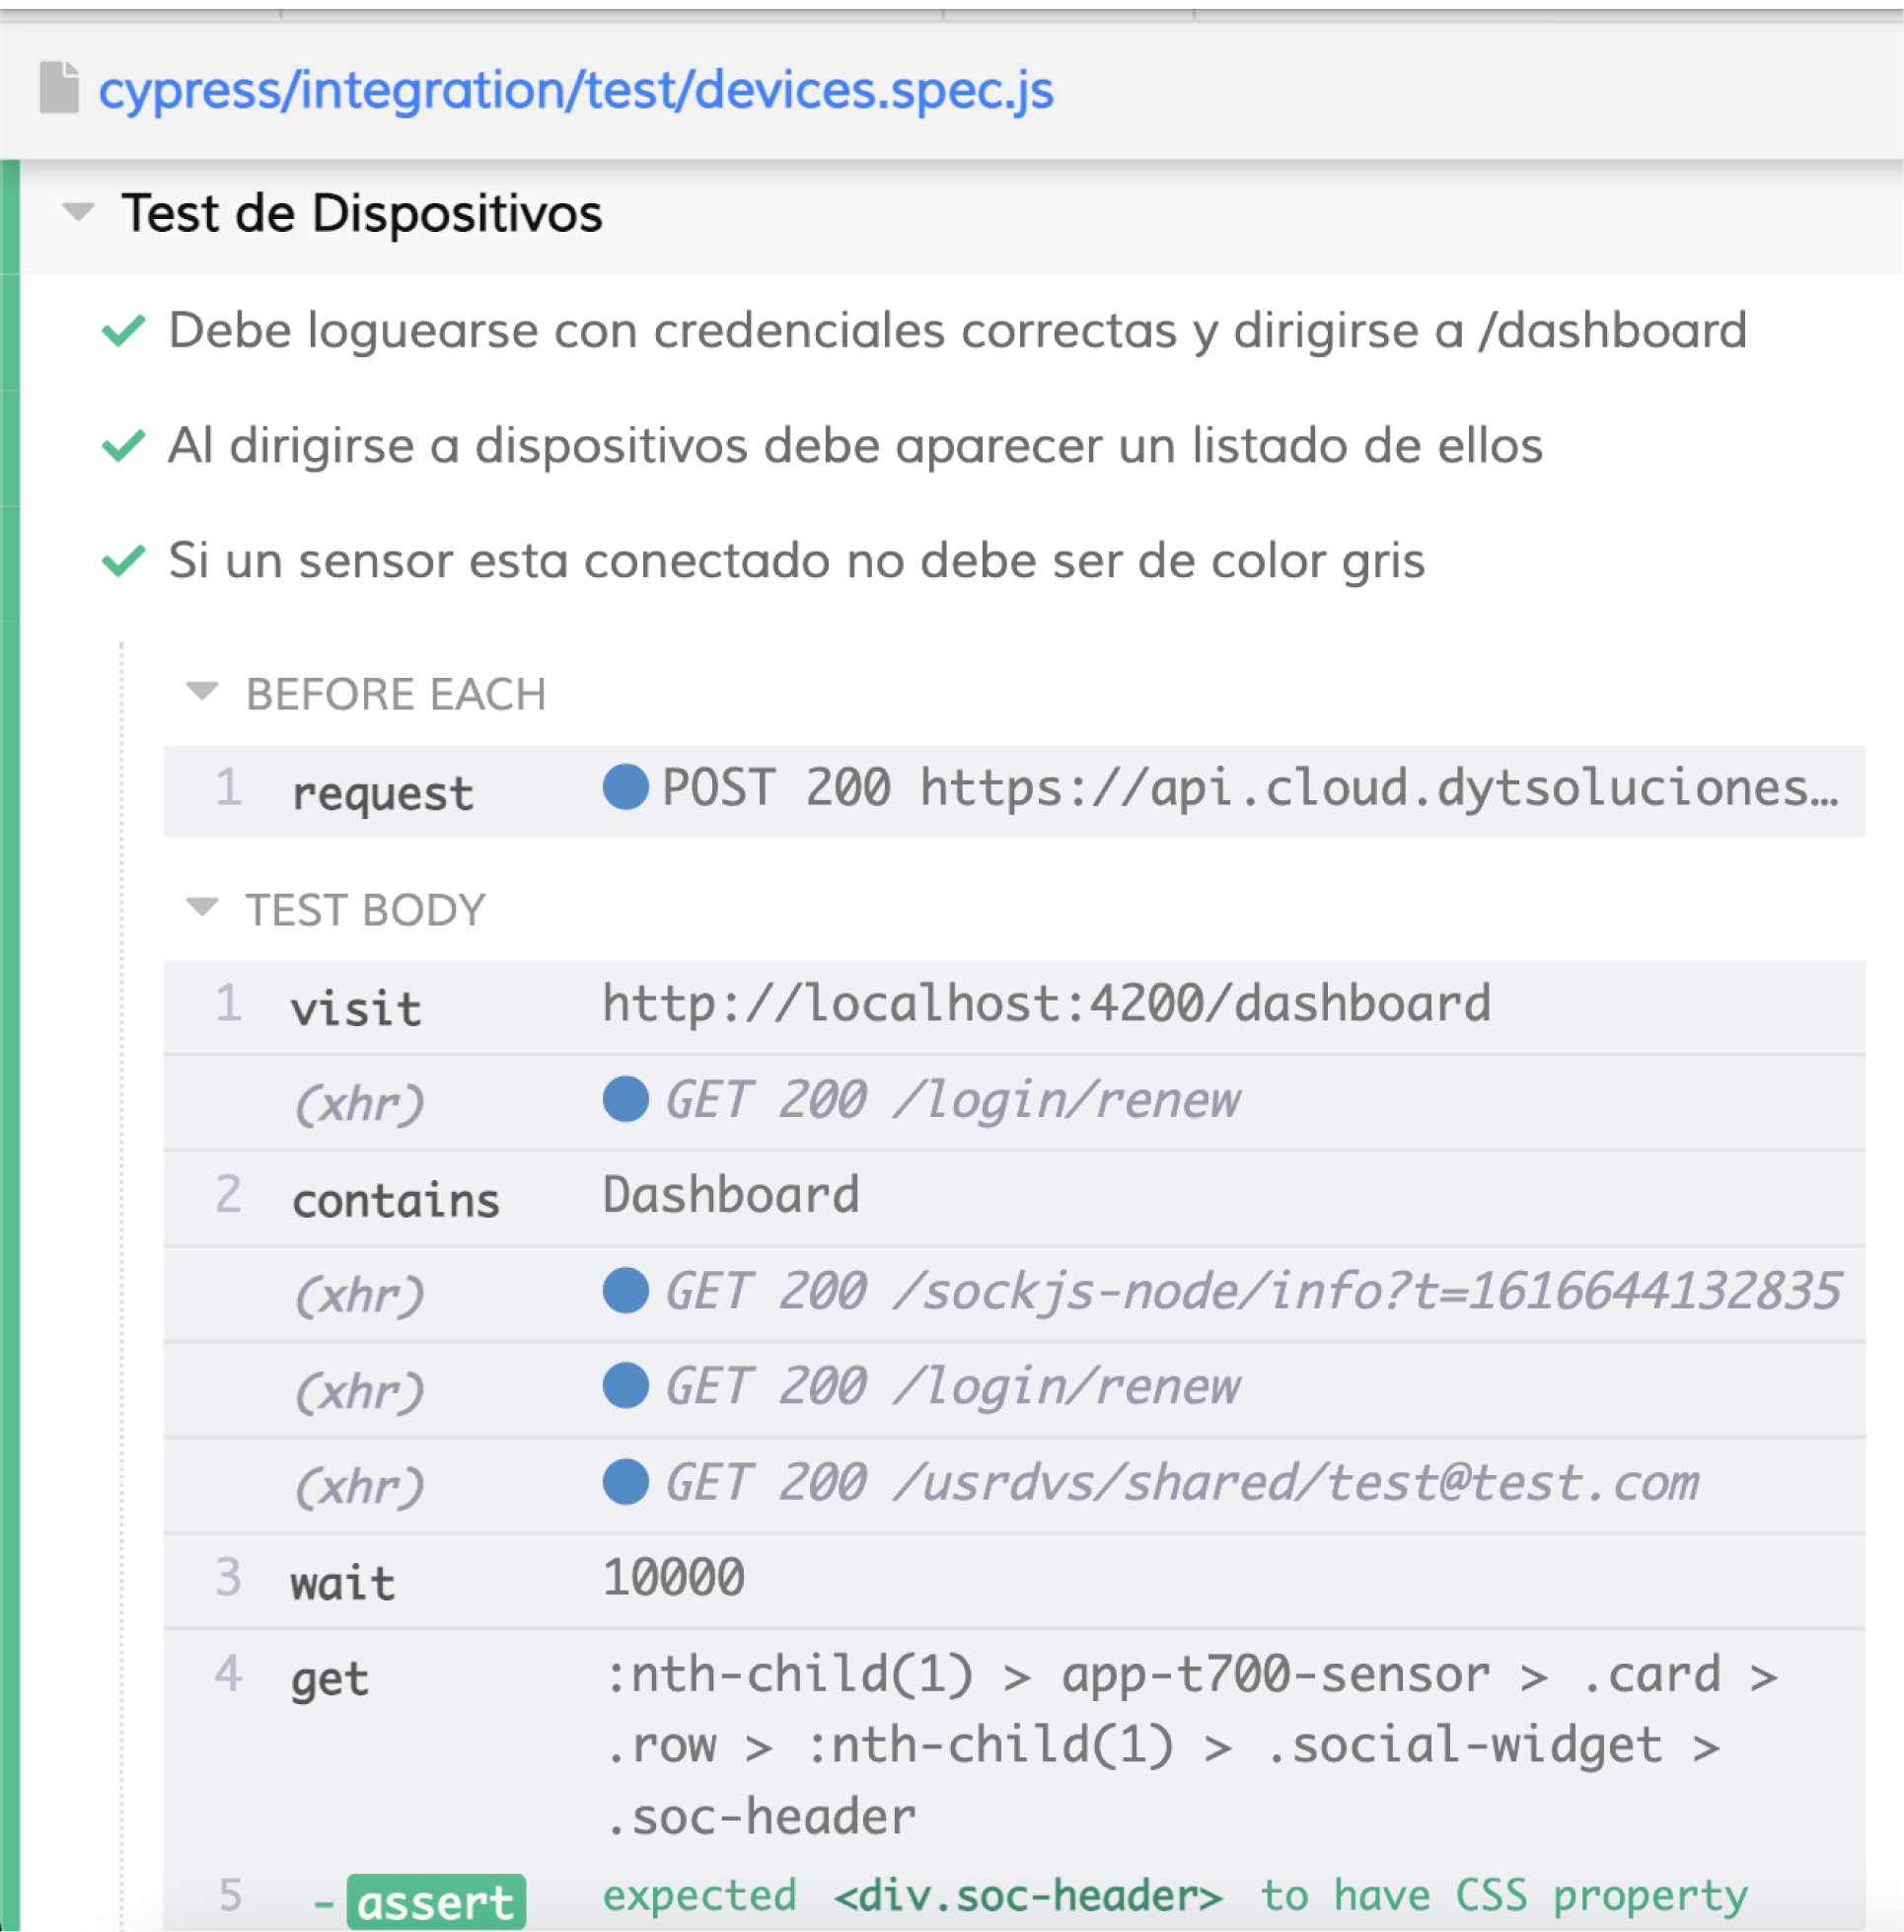
\includegraphics[scale=.60]{./Figures/test-devs-cypress.png}
	\caption[Resultado de test de dispositivos de la plataforma web]{Ilustración del entorno web de Cypress con los resultados de los test realizados a dispositivos asociados a un usuario de la plataforma.}
	\label{fig:cypress-test-devs}
\end{figure}

\pagebreak
Es importante mencionar que se realizó el test de cambio de color del componente de un dispositivo para poder determinar de manera indirecta que el dispositivo está recibiendo datos del broker MQTT.  

En la figura \ref{fig:status-devs} puede observarse los dos estados posibles que pueden tener los dispositivos que se muestran en la pantalla del \textit{dashboard}.  

\begin{figure}[htpb]
	\centering
	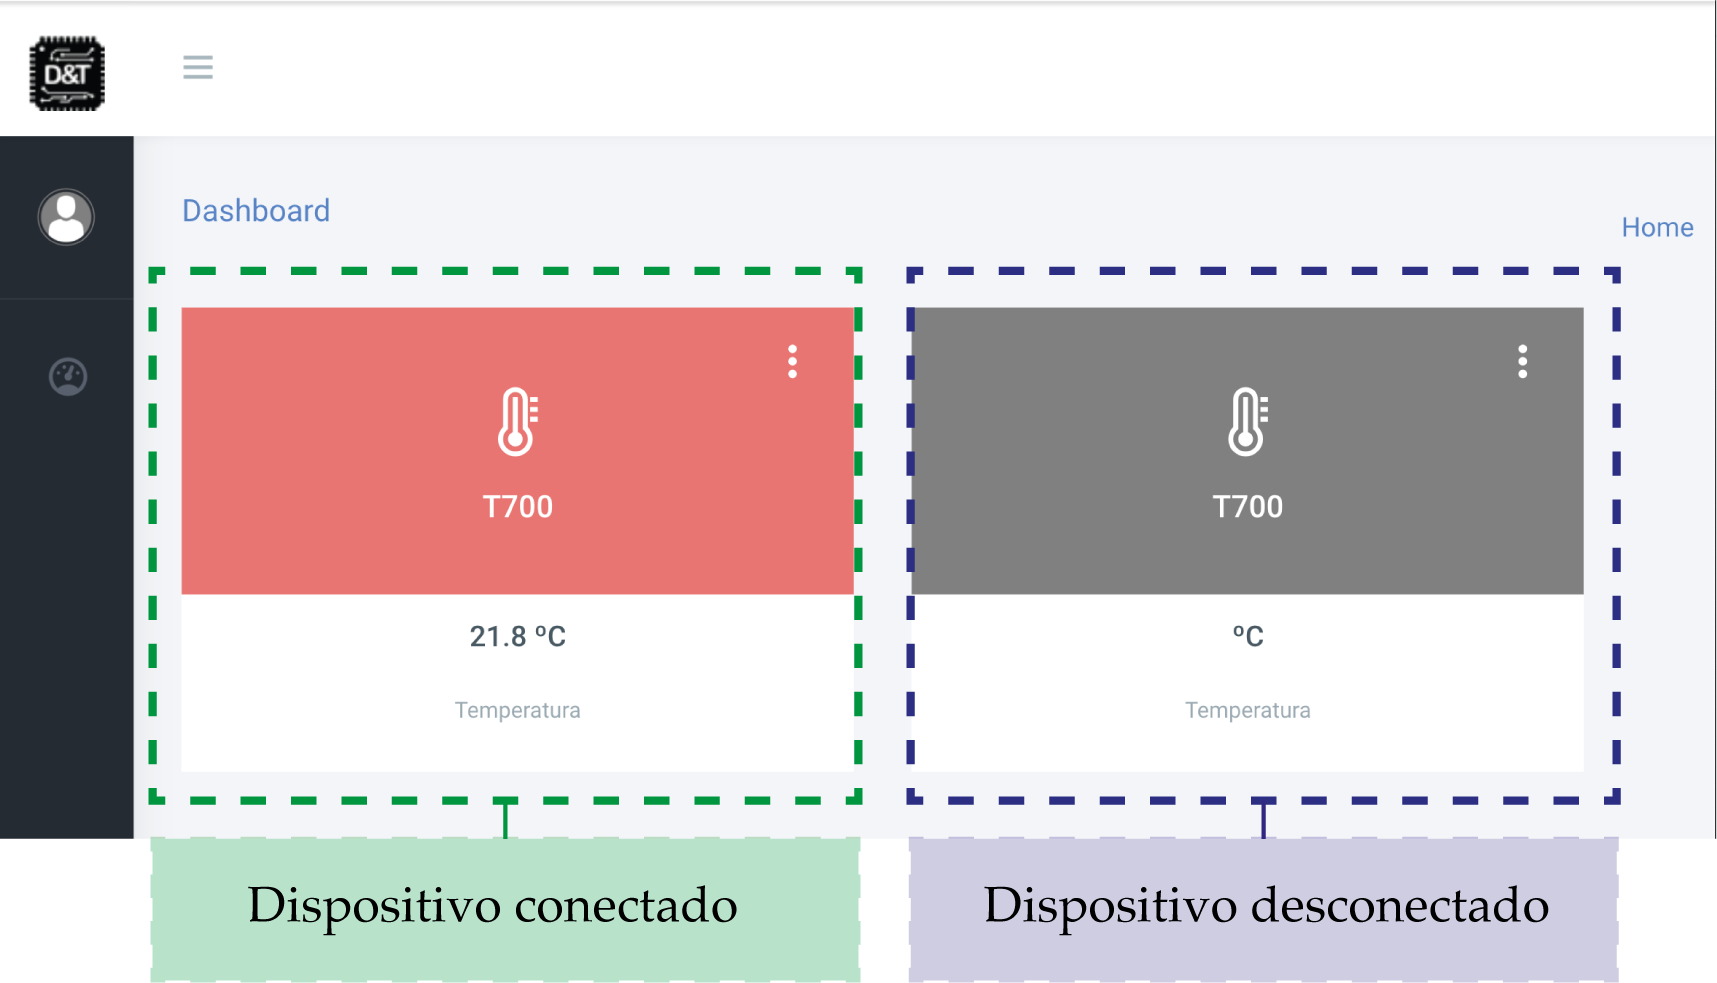
\includegraphics[scale=.75]{./Figures/estado-devs.png}
	\caption[Estados de conexión de componente de dispositivo]{Ilustración los dos estados de conexión que puede obtener el componente que identifica a los dispositivos.}
	\label{fig:status-devs}
\end{figure}

\newpage
%----------------------------------------------------------------------------------------
%	Automatizacion de test
%----------------------------------------------------------------------------------------

\subsection{Ejecución automática de tests realizados }

A fin de automatizar aún más la secuencia de tests de la sección \ref{devs-cypress} y la sección \ref{login-tests}, se agregó en los comandos de ejecución de Angular un comando de Cypress para que realice todas las pruebas que se encuentran contenidas en la carpeta creada para tal fin.  La figura \ref{fig:cmd-e2e} muestra la forma en que Angular ejecutará el comando asignado a la carpeta de test programados. 

\begin{figure}[htpb]
	\centering
	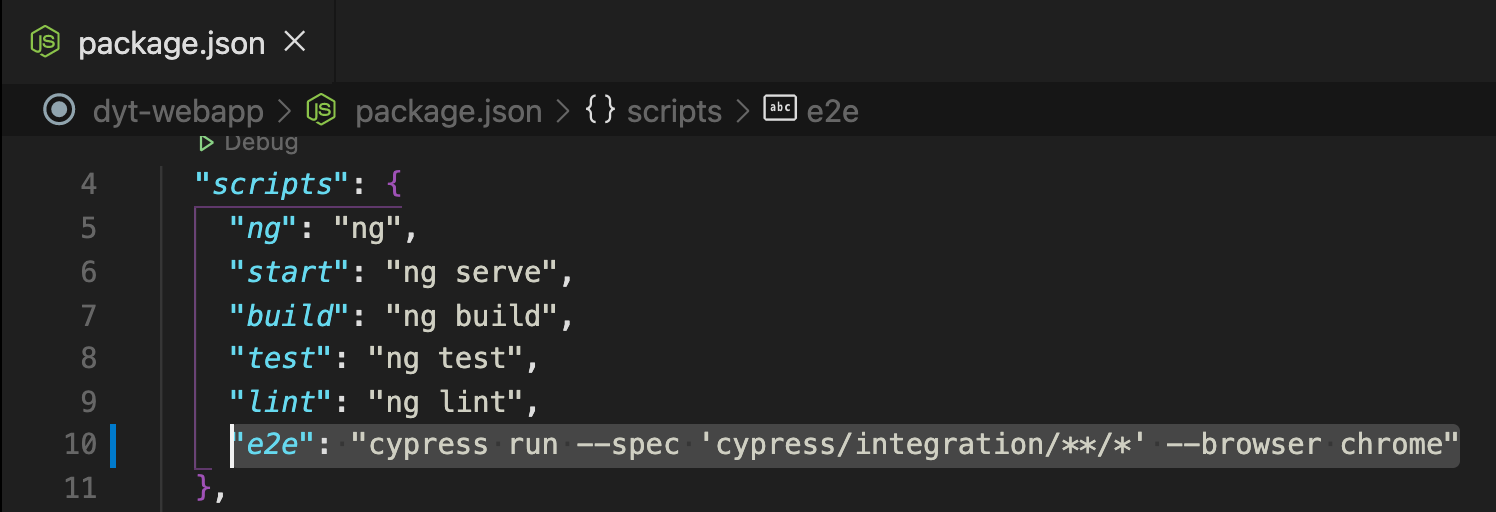
\includegraphics[scale=.50]{./Figures/cmd-e2e.png}
	\caption[Comando en Angular para ejecución de test de Cypress]{Ilustración de comando de ejecución de test e2e de Cypress en el navegador Chrome.}
	\label{fig:cmd-e2e}
\end{figure}


Para ejecutar el test completo, se ingresó el comando que se visualiza en el código \ref{cod:test-all-cypress}.

\begin{lstlisting}[label=cod:test-all-cypress,caption=Comando ejecutado para comienzo de tests programados en cypress.] 
npm run e2e
\end{lstlisting}

\pagebreak
El resultado obtenido se puede observar en la figura \ref{fig:test-all} y se concluye que el resultado de todos los tests fueron los esperados.

\begin{figure}[htpb]
	\centering
	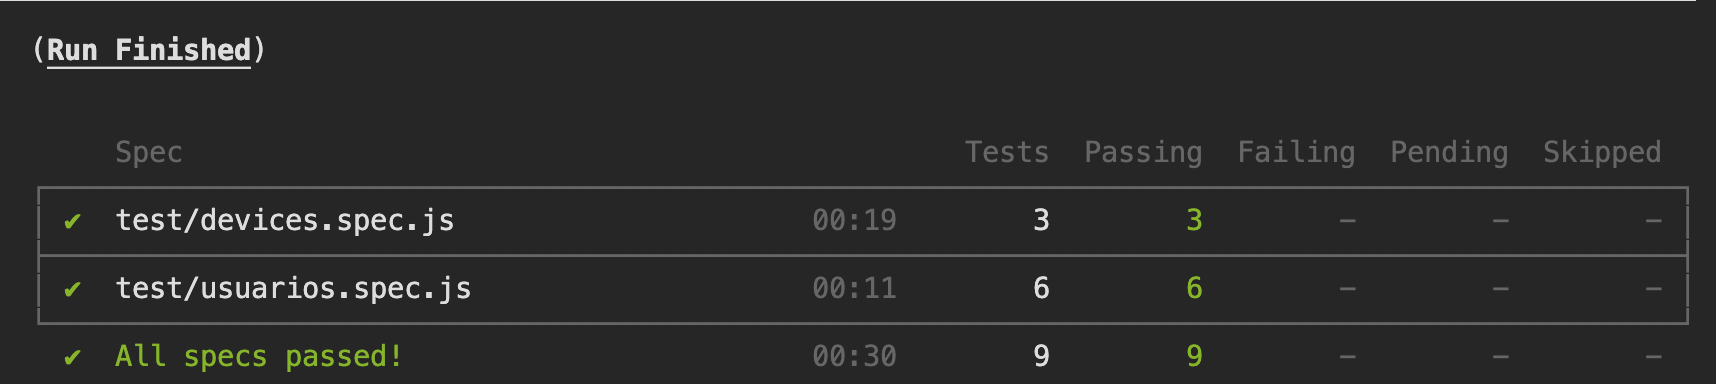
\includegraphics[scale=.45]{./Figures/test-all.png}
	\caption[Resultados de los test ejecutados en Cypress]{Ilustración de respuesta de los test ejecutados en Cypress.}
	\label{fig:test-all}
\end{figure}
 
% Chapter Template

\chapter{Conclusiones} % Main chapter title

\label{Chapter5} % Change X to a consecutive number; for referencing this chapter elsewhere, use \ref{ChapterX}

En este capítulo se presentan los aspectos más relevantes del trabajo realizado y
se mencionan los pasos a seguir.

%----------------------------------------------------------------------------------------

%----------------------------------------------------------------------------------------
%	SECTION 1
%----------------------------------------------------------------------------------------

\section{Trabajo realizado}

Se desarrolló e implementó un sistema de gestión de dispositivos conversores de protocolo Modbus a MQTT conectados a sensores de temperatura. La plataforma web demostró ser útil para el análisis del comportamiento de los sensores frente a las variaciones diarias de uso y aplicación.  A continuación se listan los logros destacados del trabajo final:

\begin{itemize}
	\item Programación e implementación de software en el servidor de datos para la vinculación de dispositivos conversores.
	\item Implementación de certificados SSL para dotar de seguridad a todo el sistema.
	\item Desarrollo de base de datos para el almacenamiento histórico de datos enviados para su posterior análisis. 
	\item Implementación de aplicación web para visualización, análisis y control de datos enviados por diferentes dispositivos conversores.
	\item Integración en la nube del sistema de gestión. 
\end{itemize}

El grado de cumplimiento de los requerimientos fué como se tenía previsto durante la planificación ya que se pudo lograr integrar el sistema e instalarlo en un servidor remoto para realizar pruebas con clientes. Estos últimos se encuentran ensayando los dispositivos conversores de protocolo Modbus a MQTT conectados a sensores de temperatura para el monitoreo del funcionamiento de cámaras frigoríficas.

Fue necesario contratar un servicio de servidor en la nube y un servicio de hosting web para poder realizar las pruebas de forma remota y que diferentes personas puedan probar el sistema. Esto llevó a un pequeño atraso en el desarrollo ya que se debió estudiar nuevos conceptos de programación y configuración de estos servicios. 

Durante el desarrollo de este trabajo final se aplicaron conocimiento adquiridos a lo largo de todo el año de la Especialización en Internet de las Cosas. Todas las asignaturas cursadas aportaron conocimientos necesarios y experiencia para la práctica profesional en el área del desarrollo web.  Sin embargo, se resaltan a continuación aquellas materias de mayor relevancia para este trabajo:

\begin{itemize}
	\item Gestión de Proyectos: la elaboración de un plan de proyecto para organizar el trabajo final, facilitó la realización del mismo y evitó demoras innecesarias. 
	\item Protocolos de Internet: se aplicaron conceptos aprendidos para la programación del servidor con los protocolos MQTT y HTTP.
	\item Desarrollo de aplicaciones multiplataforma: se adquirieron conocimientos de programación para la plataforma web adaptable a cualquier dispositivo que pueda ejecutar un navegador web.
	\item Arquitectura de datos: se desarrolló la base de datos teniendo en cuenta las especificaciones y técnicas aprendidas. 
	\item Ciberseguridad en IoT: se utilizaron técnicas de seguridad para proteger al sistema frente a posible ataques cibernéticos. 
	\item Testing de Sistemas de Internet de las Cosas: se aplicaron los conocimientos adquiridos durante la materia, sobre todo en las áreas de testing unitarios y ensayos de integración del sistema.
\end{itemize}


%----------------------------------------------------------------------------------------
%	SECTION 2
%----------------------------------------------------------------------------------------
\section{Próximos pasos}

Resulta imprescindible identificar el trabajo futuro para dar continuidad al esfuerzo realizado hasta el momento y poder realizar un sistema comercialmente atractivo. A continuación se listan las líneas de trabajo más trascendentes:

\begin{itemize}
	\item Desarrollo de notificaciones y alertas al usuario ante posible eventos configurables.
	\item Lectura de dispositivos que no pertenezcan a la medición de temperatura.
	\item Agregar un nivel de gestión de organizaciones para permitir a un usuario ser parte de varias de ellas. 
	\item Contratación de un servicio de servidor remoto de produccion para asegurar la disponibilidad, integridad y utilización de recursos del software implementado.
\end{itemize}
 

%----------------------------------------------------------------------------------------
%	CONTENIDO DE LA MEMORIA  - APÉNDICES
%----------------------------------------------------------------------------------------

\appendix % indicativo para indicarle a LaTeX los siguientes "capítulos" son apéndices

% Incluir los apéndices de la memoria como archivos separadas desde la carpeta Appendices
% Descomentar las líneas a medida que se escriben los apéndices

%\include{Appendices/AppendixA}
%\include{Appendices/AppendixB}
%\include{Appendices/AppendixC}

%----------------------------------------------------------------------------------------
%	BIBLIOGRAPHY
%----------------------------------------------------------------------------------------

\Urlmuskip=0mu plus 1mu\relax
\raggedright
\printbibliography[heading=bibintoc]

%----------------------------------------------------------------------------------------

\end{document}  
